\documentclass[10pt, a4paper, twoside, twocolumn, openright]{book}
\parindent0pt  \parskip5pt             % make block paragraphs

%\usepackage{mathtools}
%\usepackage{algorithm2e}
%\usepackage{comment}
%\usepackage[utf8]{includeenc}
%\usepackage{amssymb}
%\usepackage{amsfonts}
%\usepackage[utf8]{includeenc}
%\usepackage{subcaption}
%\usepackage[markers,nolists]{endfloat}
%\captionsetup{compatibility=false}

\usepackage{amsmath, amssymb}
\usepackage{booktabs}
\usepackage{graphicx}
\usepackage{fancyhdr}
\usepackage{subcaption}
\usepackage{titlesec}
\usepackage[english]{babel}
\usepackage[font=footnotesize,labelfont=bf]{caption}
\usepackage[super, sectionbib]{natbib}
\usepackage{chapterbib}

\exhyphenpenalty=100000

\pagestyle{fancy}
\fancyhead{}% clear headers
\fancyfoot{}% clear footers

\numberwithin{equation}{chapter}
\fancyhead[LE,RO]{\leftmark}
\renewcommand{\chaptermark}[1]{\markboth{\thechapter. \MakeUppercase{#1}}{}}
\fancyfoot[RO, LE]{Page \thepage}

\newcommand{\on}{\operatorname}
\newcommand{\rv}{\tilde}
\newcommand{\R}{\mathbb{R}}
\newcommand{\N}{\mathcal{N}}
\newcommand{\rpm}{\raisebox{.2ex}{$\scriptstyle\pm$}}
\newcommand{\argmax}{arg\,max}
\newcommand{\argmin}{arg\,min}

\newcommand{\chapterbib}{
    \bibliographystyle{ieeetr}
    \bibliography{bibliography}
    }

\titleformat{\chapter}[display]{\bfseries \LARGE}{Chapter \thechapter}{0pt}{}[\rule{\textwidth}{0.3pt}]
\titleformat{\section}[block]{\bfseries \large}{\thesection.}{3pt}{}[\vspace{-12px}\rule{0.49\textwidth}{0.3pt}]
\titleformat{\subsection}[block]{\bfseries \normalsize}{}{0pt}{\vspace{-10px}}[]

\titlespacing{\section}{0pc}{15px}{0pc} %left top ..
\titlespacing{\chapter}{0pc}{0px}{1pc}

\title{Gallardo's Thesis}
\author{Gallardo Guillermo}
\date{\today}

\begin{document}
\bibliographystyle{ieeetr}

\frontmatter
    \maketitle
    \tableofcontents
    \chapter{Dedications}
To my family, with love



\mainmatter
    \chapter{Introduction}

Composed by billions of interconnected neurons, the brain is the most complex
biological machine that we know. Understanding how brain connectivity is 
organized, and how this constrains brain functionality is one a key question
of neuroscience. Recent advances in acquisition and modeling techniques on
Diffusion Magnetic Resonance Imaging (dMRI) have facilitated to estimate and
study axonal connectivity in vivo. In this thesis, we leverage recent advances
in dMRI and tractography algorithms in order to study: how brain's connectivity
is organized; how connectivity is related to anatomy and function; how to
find correspondences when the connectivity variates across people, and how to
infer connectivity in the presence of a brain's pathology. The thesis is
divided in three major contributions:

Our first contribution is a parsimonious model for the long-range axonal
connectivity (extrinsic connectivity), and an efficient technique to divide the
brain in regions with homogeneous connectivity~\cite{Gallardo2017a}. Our
connectivity model is based on histological results obtained in the macaque
brain, and accounts for the across-subject variability in the human brain
connectivity. Our parceling technique uses a hierarchical clustering approach,
letting us comprise multiple granularities of the same brain parcellation.
Also, our technique can create both single subject and groupwise parcellations
of the whole cortex, allowing to study brain connectivity at the single subject
and at the population level. While our technique is solely based on the brain's
structural connectivity, our resulting parcels are in agreement with anatomical,
structural and functional parcellations extant in the literature. Our technique
helps to lower the gap between structural connectivity and brain function, since
some of our pure structural parcels show good overlapping with responses to
functional tasks.

Our second contribution is a technique to find correspondence between
structural parcellations of different subjects~\cite{Gallardo2018}. Even when
produced by the same technique, parcellations tend to differ in the
number, shape, and spatial localization of parcels across subjects. Matching
these parcels across subjects is an open problem in neuroscience. To solve
it, we propose a parcel matching method based on Optimal Transport. We test its
performance on different parcellations, and compare it against state of the
art matching techniques. We show that our method achieves the highest number
of correct matches. Our technique could help to study properties of structurally
defined areas, when they do not have high spatial coherence across subjects.
Also, it could help to understand the link between different brain atlases, and
improve the comparisons of cortical areas between higher primates.

Our third contribution is a multi-atlas technique to infer the location of 
white-matter bundles in patients with a brain pathology~\cite{Guillermo2018}.
Lesions in the cortex or white matter disrupt the normal functioning of the
brain. Some white matter pathologies, such as tumors or traumatic brain injury,
hampers tractography, difficulting to infer which pathways are affected. We 
present a technique that infers the affected tracts by aggregating spatial
information from healthy subjects while taking into account the diffusion
information of the patient. In particular, we register the tracts of each
healthy subject to the patient, and make each healthy patient 'vote' for a
tract on each voxel of the DWI image of the patient. Our technique weights the
vote of each subject based on how the voted pathway is supported by the patient's 
diffusion data. This is, if the diffusion data of our patient is consistent with
the direction of the voted pathway, the vote has a higher weight. We show that
our technique achieves better results that using the simple voting.

%The human brain is the most complex biological machine known in the universe.
%The brain works as a complex network of billion of neurons.
%Since this is impossible to handle, we need to subdivide the brain.
%Depending how you look at it, the brain can be divided following many different criteria (cytho, function).
%In each one of these criteria, brain connectivity is quite important and consistent.
%We know this thanks to invasive stuff.
%Since our brain is the result of biological evolution, we tortured monkeys, cats and rats in order to study and understand it.
%We cannot do that anymore, so it's difficult to study brain connectivity.
%Diffusion MRI allows to study the brain invivo without inducing pain/problems.
%But it has strong limitations: resolution in time and space, directionality, etc.
%It has been used to divide the brain, but the techniques are not good enough.
%We don't know how many parcels we need, or how to do it.
%We propose a parcellation technique that solves many of these problems.
%We show it is consistent with function.
%Now we would like to use this to study brain connectivity and function in different subjects.
%However, an interesting problem is that, for some regions, as frontal cortex, there's a lot of across subject variability.
%Turns out that it's hard to match parcels across subjects.
%Spatial overlap does not work here because of [cite].
%We need to match stuff while imposing few constraints, specially spatial ones.
%The existing techniques are nice and simple, but not sufficient.
%We propose to improve the matching by using optimal transport.
%It actually works well.
%Now that we have a way to parcellate the brain, and a way to map that across subjects, maybe we can better study the structure-function relationship.
%I would like to talk about predicting function from structure.
%This would be a negative chapter, since we were not able to predict anything from tractography.
%But, what happens when there's a pathology in the white matter?
%It's affecting brain function, but we cannot precisely predict what since it impedes tractography.
%In that case, we need to do something to infer which bundles are affected.
%We can do multi-atlas stuff.
%Since bundles are related to dmri, we can add dMRI information to the multi-atlas to improve the localization of affected bundles.
%Finally, the structure vs function in the brain does not necessarily always have to be structural connectivity vs tfmri function.
%We can also use microstructure vs cognitive, and microstructure to function (collaboration with vinod)
%
%\section{Organization}
%I start by making a beautiful introduction to neuroanatomy, because the reader needs to know what is a brain.
%Here we talk about sulci, giri, white matter, gray matter, cellular composition, layers, etc.
%This chapter also talks about brain function, but from an old perspective.
%Then, I move to explain the state of the art of the non-invasive techniques that we're interested in.
%Since the thesis is going to be about brain parcellation, I have to explain why we are interested on it.
%So the next chapter is about well known parcellations: cytho, broadmann areas, desikan, functional... the classical ones.
%Then, I can basically take the paper of Vinod and explain that, even when we subdivide the brain in specific areas, the brain works as a network.
%There should be a big focus on Structural connectivity since it's the main theme of the thesis.
%We start again with why structural connectivity is important.
%Then, we explain again that it's important to divide the brain based on its connectivity, so we know the basic pieces of the brain that work together.
%We present my work (CDMRI + neuroimage), this includes state of the art, and I guess stuff that was made after.
%%In the previous chapter we explained how to divide the brain based on a structural criteria.
%Now, other chapter, we discuss that there's variability in the parcellation of different subjects.
%We insist in the fact that this is ok, because we are all different humans. 
%Then we present the MICCAI paper made in collaboration with Nathalie, this includes state of the art, etc etc etc
%%
%Another chapter, this time about multiatlas.
%%\section{Structure vs Function}
%Finally, something about structure vs function.
%In the intro we explained that structure is important, and that function is driven by function.
%It's time to show that this actually happens, and in which cases.
%We can start talking about Osher and others, however this didn't work for us.
%I think it's important to say it.
%%Gaston????????????
%Then, I can include the final part of my neuroimage, where we show the parcels are functionally specialized.
%Maybe something about the work with Nathalie.
%Stanford stuff goes here I guess
%New experiments.
%
%\section{Other projects?}
%Stanford vwfa? RTOP? Harvard? No idea...



%\section{Organization}
%
%\subsection{Neuroanatomy}
%
%I start by making a beautiful introduction to neuroanatomy, because the reader needs to know what is a brain.
%Here we talk about sulci, giri, white matter, gray matter, celular composition, layers...
%
%\subsubsection{Brain parcellation - Cytho}
%Since the thesis is going to be about brain parcellation, I have to explain why we are interested on it.
%I can explain about cytho, broadmann areas, desikan, functional... the classical ones
%
%\subsubsection{The brain as a network}
%Here I can basically take the paper of Vinod and explain that, even when we subdivide the brain in specific areas, the brain works as a network.
%There should be a big focus on Structural connectivity since it's the main theme of the thesis.
%
%\subsection{Non invasive methods}
%In this chapter we explain the state of the art of the non-invasive techniques that we're interested in.
% 
%\subsubsection{dMRI and tractography}
%How diffusion MRI works, from A to Z.
%Then I talk about tractography... when to use each type, advantages and disadvantages.
%
%\subsubsection{fMRI}
%A gentle introduction to fMRI, we don't need to focus a lot on this.
%
%\subsection{Background Methods}
%
%dividir en backgound y contributions
%
%\section{Structural Connectivity based parcellation}
%We start again with why structural connectivity is important.
%Then, we explain again that it's important to divide the brain based on its connectivity, so we know the basic pieces of the brain that work together.
%We present my work (CDMRI + neuroimage), this includes state of the art, and I guess stuff that was made after?
%
%\section{Matching parcels across different subjects}
%In the previous chapter we explained how to divide the brain based on a structural criteria.
%Now, we discuss that there's variability in the parcellation of different subjects.
%We insist in the fact that this is ok, because we are all different humans. 
%Then we present the MICCAI paper made in collaboration with Nathalie, this includes state of the art, etc etc etc
%
%\section{Structure vs Function}
%In the intro we explained that structure is important, and that function is driven by function.
%It's time to show that this actually happens, and in which cases.
%We can start talking about Osher and others, however this didn't work for us.
%I think it's important to say it.
%Gaston????????????
%Then, I can include the final part of my neuroimage, where we show the parcels are functionally specialized.
%Maybe something about the work with Nathalie.
%New experiments.
%
%\section{Other projects?}
%Stanford vwfa? RTOP? Harvard? No idea...
%
%\section{Conclusions}

    %'sine anatomia non sciemus' - Without anatomy there is no knowledge

%TODO
% Fix text
% add more information on fmri networks?
% talk more about evolution? [VINOD, MARS?]
\chapter{The Human Brain: An Introduction to Cytoarchitecture, Anatomy and Function}
\label{ch:intro_anato}

\section{Overview}
In this chapter we cover the basic aspects of cellular composition, morphology
and function of the human brain. We start with a brief introduction to the
human nervous system, in order to understand the biological context of the brain.
Then, we study the brain from both a microscopic and a macroscopic view. In the
microscopic view, we explain the cellular composition of the brain and how it’s
organized. In the macroscopic view, we zoom out and make a review of the most 
important divisions and anatomical landmarks of the brain. Finally, we describe
the functional role of some of these gross anatomical divisions. This chapter is
heavily based on the books: Neuroscience~\cite{Purves2004} ; Clinical
Neuroscience~\cite{Johns} and Atlas of Human Brain Connections~\cite{Catani2012}.
We encourage the reader to further deepen each subject using those books.

\section{The Human Nervous System}
Every organ in our body works as part of a larger system of organs interacting
towards a common goal. Our brain, the main actor of this thesis,
forms part of the nervous system, the system concerned with concious life.
The nervous system is the most complicated and highly organized of the various
systems which make up the human body\cite{Gray1918}. It is the mechanism
concerned with the analysis and integration of internal and external stimuli,
and with the reactions and adjustments of the organism in response to them. It
is anatomically divided into two parts, central and peripheral \ref{fig:cns_and_pns}.
The central nervous system (CNS) consist of the brain and the spinal cord. The
peripheral nervous system (PNS) consists of a series of nerves that link
receptors on the body with the central nervous system. These nerves are
associated with the functions of the special and general senses and with the
voluntary movements of the body. As a system, the PNS transmits stimuli from
the environment to circuits within the spinal cord and the brain, which are
integrated alongside internal stimuli in order to produce a response. This
response travels back trough the PNS and is translated into body movement or
the adjustment of internal organs (fig. \ref{fig:cns_and_pns}). 

\begin{figure}[h]
    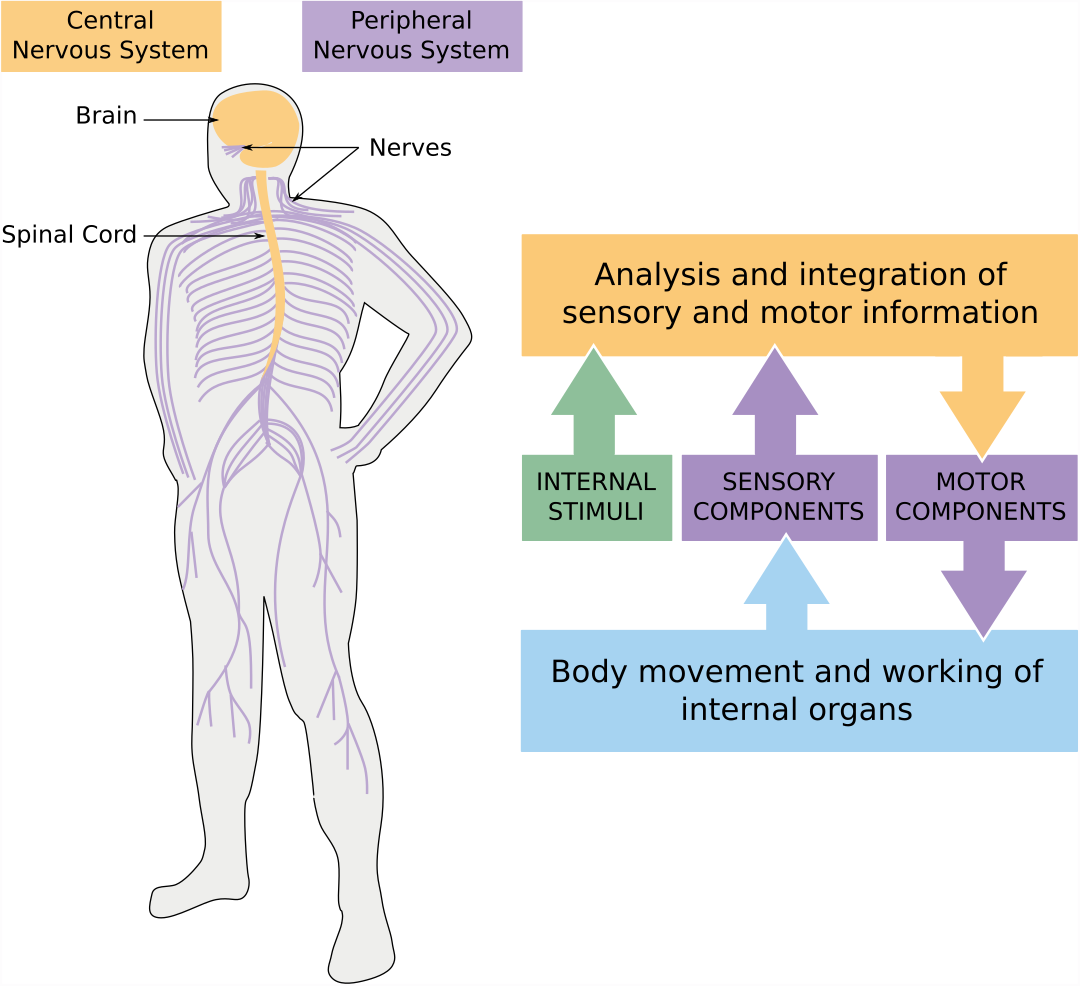
\includegraphics[width=0.49\textwidth]{2.neuroanatomy/img/pns_and_cns.png}
    \caption{The nervous system is anatomically divided in two: The central
             nervous system (CNS) and the peripheral nervous system (PNS).
             On the left we show a simplified representation of the CNS and
             PNS in the human body. On the right we schematize how these systems
             interact beween them: internal and external stimuli gathered by
             the PNS and sent to proccess to the CNS, which then decides how to
             respond. This image was adapted from the book Neuroscience~\cite{Johns}.}
    \label{fig:cns_and_pns}
\end{figure}  

In this thesis we will focus only on the brain. We start by talking about its
cellular composition and internal organization.

\section{A Microscopic View of the Human Brain}

\begin{figure*}[h!]
    \includegraphics[width=\textwidth, height=200px]{missing.png}
    \caption{Different types of neuronal and nonneuronal cells. (A) a pyramidal
             neuron, (B) granule neuron, (C) neuron with a highly complex
             arborization, (D) von Economo neuron. (E) Neuroglia, or supporting cell }
    \label{fig:neuron_types}
\end{figure*}

At a microscopical view, the human brain is composed by cells that can be
divided in two broad categories: nerve cells (or neurons), and supporting cells
called neuroglia (or simply glia). Nerve cells (Fig. \ref{fig:neuron_types} A)
are discrete entities that communicate with one another by means of specialized
contacts called “synapses”\cite{Purves2004}. Supporting cells (Fig. \ref{fig:neuron_types} E),
in contrast, are not capable of electrical signaling; nevertheless,
they have several essential functions in the developing and adult brain. The
human brain possess on average 86.06 +/- 8.12 billion neurons and
84.61 +/- 2.17 billion nonneuronal cells, making it a linearly scaled-up primate
brain in its cellular composition. In terms of distribution, 80\% of the neurons
are present in the cerebellum, and approximately all the rest are in the cortex.
Meanwhile 80\% of the nonneuronal cells are in the cortex, with almost all the
rest in the cerebellum.

% THIS NEED TO BE HERE TO MAINTAIN COHERENCE IN THE COMPILED PDF
% BUT IT'S ACTUALLY OF THE NEXT SECTION
\begin{figure*}[h!]
    \includegraphics[width=\textwidth, height=200px]{missing.png}
    \caption{Brain tissue can be divided into grey and white matter. (A) Grey matter
             is composed mainly of cell bodies. (B) White matter is made up mostly
             of packed axons.}
    \label{fig:white_grey_matter}
\end{figure*}
% 

\subsection{Neurons}

The basic cellular organization of neurons resembles that of other cells; however,
they are clearly distinguished by specialization for intercellular communication.
This attribute is apparent in their overall morphology, in the specific
organization of their membrane components for electrical signaling, and in the
structural intricacies of the contacts between neurons. The spectrum of neuronal
geometries ranges from a small minority of cells that lack dendrites altogether
to neurons with complex dendritic arborizations (i.e. Fig. \ref{fig:neuron_types} C).
The complexity of the dedritic arbor constrains the amount of neurons with who
a neuron can communicate, ranging from one or few, to a commensurately larger
number of other neurons.

From a functional point of view, we can distinguish two type of neurons:
excitatory and inhibitory. Excitatory neurons release the neurotransmitter
glutamate to send signals to other cells. Inhibitory neurons release
gamma-Aminobutryc acid, in order to reduce neuronal excitability throughout
the nervous system~\cite{Bekkers2011}.

From a morphologic point of view, neurons can be divided in two major types:
granule neurons and pyramidal neurons \cite{Purves2004}. Granule cells are 
star-shaped neurons with a typical diameter of less than 20$\mu$m. They are
multipolar neurons, this is, neurons that posses a single axon and many dendrites.
Granule cells are either excitatory or inhibitory, and mostly have purely
‘intrinsic’ axons, this is, they make only short-range, local connections~\cite{Purves2004}.
On the other hand, pyramidal neurons have large, pyramid-shape bodies that
range from 20-120$\mu$m. Pyramidal neurons are multipolar and excitatory neurons,
and they comprise about two-thirds of all neurons in the mammalian cerebral cortex.
On top of their numerical dominance, pyramidal neurons are also 'projection neurons',
meaning that they axons are often 'extrinsic', making long connections~\cite{Purves2004}.

Finally, neurons on a circuit can be classified based on their role in a 
neuronal circuit. Nerve cells that carry information toward the circuit are
called afferent neurons; nerve cells that carry information away from the 
circuit are called efferent neurons. Interneurons, or local circuit neurons,
only participate in the local aspects of a circuit.

%Another important type of neurons to this thesis are the spindle neurons \cite{Johns}.
%Spindle neurons, also called von Economo neurons (VENs), are a specific cfass of
%neurons that are characterized by a large spindle-shaped soma (or body),
%gradually tapering into a single apical axon in one direction, with only a
%single dendrite facing opposite. VENs emerged within the last decade as having
%a potentially major role in self-awareness and social cognition in humans \cite{Evrard2012}.

\begin{figure*}[t]
    \includegraphics[width=\textwidth, height=200px]{missing.png}
    \caption{The cerebral cortex is characterize by its convoluted folds.
             Some landmarks are consistent across brains, as the central sulcus;
             lateral sulcus; parieto-occipital notch and pre-occipital notch.
             These landmarks help divide the hemispheres into lobes.}
    \label{fig:cortex_anatomy}
\end{figure*}

\subsection{Neuroglial}
Neuroglial cells are quite different from nerve cells. Glial cells do not
participate directly in synaptic interactions and electrical signaling, but
instead provide support to define synaptic contacts and maintain the signaling
abilities of neurons~\cite{Purves2004}. The term glia (from the Greek word
γλοιός meaning “glue”) reflects the nineteenth-century presumption that these
cells held the nervous system together in some way. The term has survived 
despite the lack of evidence that glia actually bind neurons together. Glial
roles that are well-established include maintaining the ionic milieu of nerve
cells, modulating the rate of nerve signal propagation, modulating synaptic
action by controlling the uptake of neurotransmitters at or near the synaptic
cleft, providing a scaffold for some aspects of neural development, and aiding
in the recovery from neural injury~\cite{Purves2004}.

\subsection{Neuronal Organization: Cortical Layers}

Brain cells are arranged in horizontal layers, or laminae~\cite{Waehnert2014}.
More than 90\% of the cerebral cortex has a characteristic six-layered composition\cite{RandS.SwensonM.D.2006}.
Layer I is the molecular
layer, which contains very few neurons; layer II the external granular layer;
layer III the external pyramidal layer; layer IV the internal granular layer;
layer V the internal pyramidal layer; and layer VI the multiform, or fusiform
layer. Each cortical layer contains different neuronal shapes, sizes and density
as well as different organizations of nerve fibers\cite{RandS.SwensonM.D.2006}.
The layer structure varies spatially in regard to cell organization (cytoarchitecture) and 
myelination (myeloarchitecture), defining distinct cortical areas which are
likely to perform different functions \cite{Waehnert2014, Bok1929}. 

Depending on the layers present, the cortex can be divided in agranular,
disgranular and granular regions\cite{Mesulam1982}. The agranular cortex is characterized by not
having a internal granule cell layer (layer IV). The granular cortex has two 
layers of granule cells, an external granular layer (II) and an internal granular
layer (IV). Dysgranular cortex has fewer granule cells, which are grouped in a
single layer or as distinct clusters.

The fine study of the cortical composition is called Cytoarchitectonics. We 
discuss the topic of parcelling the brain based on cytoarchitecture in chapter
4, now it's sufficient to say that the cerebral cortex is divided into more than
fifty regions based on its cellular composition under the microscope. The most
known and frequently cited cythoarchitectural organization is that of
Brodmann~\cite{Brodmann1909} (Fig. \ref{fig:brodmann_small}).

\begin{figure}[h]
    \includegraphics[width=0.49\textwidth, height=150px]{missing.png}
    \caption{The cerebral cortex is divided into more than 50 regions based on
             its cellular composition. Brodmann's\cite{Brodmann1909}
             parcellation is the most known and cited one.}
    \label{fig:brodmann_small}
\end{figure}

\section{A Macroscopic view of the Human Brain}
In the previous section, we talked about neurons and how they are specialized
to transmit information. Indeed, neurons never function in isolation; they are
organized into circuits or structures that process specific kinds of information.
The brain tissue comprises a diverse collection of these neural structures,
each with a distinctive shape and an intricate internal architecture.

Brain tissue can be divided into grey and white matter~\cite{Johns} (Fig. \ref{fig:white_grey_matter}).
Grey matter is composed mainly of neuronal cell bodies, dendrites and synapses.
It is sharply demarcated from the adjacent white matter, which is made up mostly
of axons travelling from grey matter to grey matter, or to other parts of the
nervous system. The pale colour of white matter is due to the lipid-rich myelin
sheath that surrounds axons and enhances their conduction velocity\cite{Johns}.


\subsection{Anatomy of the Grey Matter}

The grey matter is composed of: the cerebral cortex; the cerebellum; structures
within the white matter, called subcortical structures (i.e. thalamus; hypothalamus; etc),
and the grey column, which traverses the spinal cord. In this thesis we will
mainly focus on the cerebral cortex.

The cerebral cortex is the most important structure of the gray matter and
plays a major role in cognitive functions. It is a layered sheet of tissue,
2–3 millimetres thick, with highly convoluted folds. It's hypothesized that the
mechanical tension created by neuronal connections during development is a major
driving force of these folds~\cite{VanEssen1997}. An advantage of the folding
pattern, is that it allows to fit a large surface area within the available
cranial volume. In particular, the human cerebral cortex attains a surface area
of about 1600 $cm^2$, nearly three times what it would be in the absence of
convolutions~\cite{VanEssen1997}. The grooves and ridges created by this folding
process are called sulci and gyri respectively.

The cerebral cortex is divided in two hemispheres by a prominent central fissure.
The hemispheres are characterized by the gyri (singular, gyrus) or crests of
folded cortical tissue, and sulci (singular, sulcus) the grooves that divide
gyri from one another. Although gyral and sulcal patterns vary from individual
to individual, there are some fairly consistent landmarks, particularly the: 
central sulcus; lateral sulcus; parieto-occipital notch and pre-occipital notch.
These landmarks help divide the hemispheres into four lobes: occipital, 
temporal, parietal, and frontal. Hidden from surface view is the fifth lobe:
the insular lobe. Figure \ref{fig:cortex_anatomy} presents a illustration of this.

\subsection{Anatomy of the White Matter}

\begin{figure*}[t]
    \includegraphics[width=\textwidth, height=200px]{missing.png}
    \caption{Example of three major tracts in the white matter. (Red) The Corpus
             Callosum is a commisural pathways that communicates both hemispheres.
             (Green) The Inferior Longitudinal Fasciculus is an association tract
             that communicates the temporal with the occipital lobe. (Blue) The
             Internal Capsule is a projection tract connecting the Thalamus
             with the cortex.}
    \label{fig:white_anatomy}
\end{figure*}

Axons in the central nervous system are gathered into bundles of different
diameter, and several bundles form larger pathways called fasciculi, or tracts~\cite{Catani2012}.
Most of the cerebral fibers forming the white matter connect distant regions 
within the cortex. Others, connect cortical region with the peripherical nervous
system or subcortical structures. There are some fibers, the less, that connect
only subcortical structures.

Some of the major bundles running along the white matter are well defined in the
modern neuronanatomy. Examples of major bundles in the human brain are the
Corpus Callosum, the Internal Capusule and the Superior Longitudinal Fasciculus
(Fig. \ref{fig:white_anatomy}.)
The Corpus Callosum is the largest tract of the human brain, composed of some
200–300 million myelinated axons it connects both hemispheres, allowing to
transfer information from one to another~\cite{Catani2012}. The internal capsule
contain ascending fibres mainly from the thalamus to the cortex, and descending
fibres from the cortex to subcortical structures, and the spinal cord~\cite{Catani2012}.
This complex projection system conveys sensorial information to the cortex and 
controls movement. Our last example, the Inferior Longitudinal Fasciculus, is
a tract with long and short fibres connecting the occipital and temporal lobes~\cite{Catani2012}.
Its involved in visual and language functions.


\subsection{Neuroanatomical Naming Conventions}

\begin{figure*}[t]
    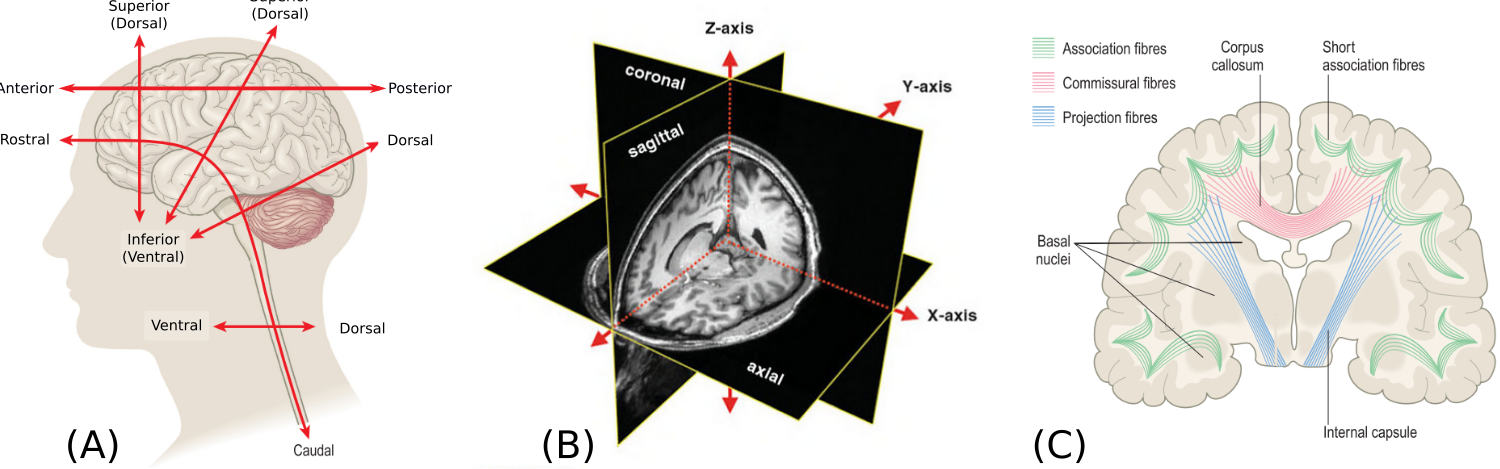
\includegraphics[width=\textwidth]{2.neuroanatomy/img/terminology.png}
    \caption{Terms commonly used to describe the orientation of the brain in surface (A), sectional (B) and connectional anatomy (C) representations.}
    \label{fig:anatomy_terminology}
\end{figure*}

In order to describe the location of structures on the brain, standardized
nomenclature is used. Brain's anatomy can be described from its surface,
from orthogonal sections that traverse the brain, or from its white matter~\cite{Catani2012}.

The surface of the brain can be viewed from the side (lateral view),
the middle (medial view), the front (anterior or frontal view), and the back
(posterior or occipital view)~\ref{fig:anatomy_terminology}. The same terminology
is used to indicate different regions of the brain surface (e.g. dorso-lateral prefrontral cortex).

Sectional neuroanatomy describes the relationship between cortical and
subcortical structures, most commonly visualized along orthogonal axial,
coronal, and sagital planes~\ref{fig:anatomy_terminology}. In radiological
convention, the axial slices are viewed from the feet towards the head.
The coronal planes are conventionally oriented with the left side of the brain
on the right side of the page (frontal view). Finally, the sagittal plane 
divides the brain into two hemispheres.

White-matter neuroanatomy delineates the origin, course, and termination of
connecting pathways~\ref{fig:anatomy_terminology}. The tracts are classified
according to their course and terminal projections. Commisural pathways run
along a horizontal axis and connect the two hemispheres. The majority of the
projection pathways have a perpendicular course along a dorso-ventral
(descending) or ventro-dorsal (ascending) axis and connect the cerebral
cortex to subcortical nuclei, cerebellum, and the spinal cord. The association
tracts run longitudinal along an antero-posterior axis and connect cortical 
areas within the same hemisphere.

These gross descriptions of some prominent anatomical landmarks provide a
framework for naming, locating and studying different brain structures. Being
able to locate brain regions in different subjects is a necessary first step
to study the basic of brain function.

\section{Brain Function}

\begin{figure*}[t]
    \includegraphics[width=\textwidth,height=150px]{missing}
    \caption{(A) Different regions of the brain are specialized for different
             functions, most of them where mapped based on the postmortem 
             examination of brain lesions in subjects with functional
             deficiencies. (B) Closer look to the motor and sensory cortex.}
    \label{fig:brain_function}
\end{figure*}


While we know that concious emerges from the brain, we still have a long path
ahead to unravel how the brain works. So far, and thanks to the study of
brain lesions, many motor and cognitive functions have been mapped to coarse
brain regions (Fig. \ref{fig:brain_function}). In this section, we present an
overview of the general function attributed to each lobe, while introducing 
some of the functional subdivisions used later on this thesis.

\subsection{Frontal Lobe}
The frontal lobe is responsible for motor functions, speech production, 
planning, personality, insight and foresight.

One of its divisions, the precentral gyrus (Fig. \ref{fig:brain_function} A),
contains an inverted point-to-point map of the motor functions of the opposite
half of the body (Fig. \ref{fig:brain_function} B)~\cite{Johns, Purves2004,
Catani2012}. This area is called the primary motor cortex, and corresponds to
Brodmann's region 4. It was mapped by Penfield et al.~\cite{Penfield1954} trough
experimenting with electrical stimulation. A remarkable fact is that the area
allocated for each body part is proportional to the precision of movement
control~\cite{Johns}. In particular, the areas for the hands, face and tongue
are disproportionately large (Fig. \ref{fig:brain_function} B).

The region in front of the primary motor cortex is the lateral premotor area.
Defined as the Brodmann Area 6, it does not correspond to any particular gyral
or sulcal boundaries~\cite{Johns, Purves2004}. The premotor cortex also contains
an inverted body map and is concerned with preparation and execution of movement
sequences in response to external stimuli (as catching a ball, rather than throwing one)~\cite{Johns}.

The large portion of the frontal lobe anterior to the motor
and premotor areas is the prefrontal cortex and is involved in personality, 
behaviour, language and intellect~\cite{Johns}. Its mainly concerned with
organizing and planning behaviour in pursuit of short-, medium- and long-term goals.
It also has a cognitive inhibitory role, preventing inappropriate behaviour~\cite{Sigman2017}.

Finally, the opercular and triangular parts of the inferior frontal gyrus
(Brodmann Areas 44 and 45) correspond to Broca’s area. This area is involved in
the expressive aspects of spoken and written language (production of sentences
constrained by the rules of grammar and syntax)~\cite{Johns}. The area was named
after Pierre Paul Broca, who reported speach production impairments in two patients.
This area tends to be lateralized to the hemisphere in charge of the dominant
hand. 

\subsection{Parietal Lobe}
The parietal lobe is responsible for language comprehension, spatial orientation
and perception, and somatic senses, such as touch and temperature.

Located on the parietal lobe, immediately posterior to the centrar sulcus, and
parallel to the precentral gyrus, there is the postcentral gyrus. It corresponds 
to the primary somatosensory cortex (BA 3, 1 and 2). The sensory cortex contains
an inverted map of the opposite side of the body that mirrors that of the motor
cortex, but the relative proportions of the body parts reflect the degree of 
tactile sensitivity~\cite{Johns}.

\subsection{Occipital Lobe}
The occipital lobe is concerned entirely with visual processing and association.
It contains the Brodmann Area 17, which correspondes to the primary visual cortex.
The primary visual cortex is highly specialized for processing visual information, and
possess a point-to-point (retinotopic) representation of the visual field~\cite{Johns}.
The visual system continues in the visual association cortex (BA 18 and 19),
which helps in the detection of complex patterns and are believed to contribute
in detecting global motion~\cite{Johns, Purves2004}.

\subsection{Temporal Lobe}
The temporal lobe is involved in hearing, speech comprehension and visual recognition.

Contained by it is the auditory cortex (Fig. \ref{fig:cortex_anatomy}), which 
has a tonotopic map representing the audible frequency spectrum (low frequencies
laterally, high frequencies medially)~\cite{Johns}. More ventral is the fusiform
gyrus, which is involved in the recognition of complex visual patterns, as tools
or human faces~\cite{Saygin2011}. Another region, Wernicke’s area, corresponds to the 
posterior third of the superior temporal gyrus (Fig. \ref{fig:brain_function}) and
it's involved in language comprehension~\cite{Johns}. 

\subsection{Insula}
The insular cortex is hidden in the depths of the lateral sulcus (Fig.
\ref{fig:cortex_anatomy}). The insula is involved in attention, and in the
integration of sensory, affective, and cognitive cues~\cite{Bressler2010, Johns}.

\section{Brain Networks}

So far in this introduction to neuroanatomy, we have presented brain function
as studied by the modular paradigm.
In this paradigm, a discrete and continuous piece of cortical tissue is specialized
to serve one cognitive function or to represent one essential aspect of the
information processed by it~\cite{Fuster2000}. The interaction between many
of such modules would lead to complex cognitive function. However, accumulating
evidence shows that the paradigm has serious limitations. For example, lesions
in the brain almost never derive in the loss or degradation of only one cognitive
function~\cite{Fuster2000}. Furthermore, even the functions of primary sensory
areas, long standing thought as modular, appear to be part of a network that
integrates multisensory stimuli~\cite{Ghazanfar2006}.

A new paradigm is emerging in neuroscience, that moves beyond the simplistic
one to one mapping between cognitive functions and brain regions, and instead
maps cognitive functions to large-scale networks in the brain. So far, at least
8 major core functional networks have been defined\cite{Bressler2010}:
(i) a spatial attention network anchored in posterior parietal cortex and frontal eye fields;
(ii) a language network anchored in Wernicke’s and Broca’s areas;
(iii) an explicit memory network anchored in the hippocampal–entorhinal 
complex and inferior parietal cortex; (iv) a face-object recognition
network anchored in midtemporal and temporopolar cortices; (v) a
working memory-executive function network anchored in prefrontal and
inferior parietal cortices; (vi) central-executive network anchored in
dorsolateral prefrontal cortex and posterior parietal cortex; (vii) a salience
network anchored in anterior insula and anterior cingulate cortex; and (viii)
a default mode network, a set of functional networks that emerge while a person
is resting.

Thinking the brain as a set of interacting networks, instead of single anatomical
regions, creates a sound base to study cognition\cite{Bressler2010}. However,
if a single network can be said to support a specific cognitive function is 
still an open question in neuroscience. Answering it will depend on the 
developing of new techniques to study not only brain function, but also brain
connectivity.

\section{Conclusions}
This chapter introduced the basic knowledge in neuroanatomy necessary to
understand the rest of the thesis. Moreover, it explained how the interaction
between neurons by means of connectivity drives not only the brain morphology
but also its function. It also highlighted how neuroscience is moving from
viewing the brain as a mosaic of functionally specialized regions, to an
interactive network from which cognition arises. This view of the brain as 
a network is a key aspect that drives some of the contributions of this thesis.

Most of the knowledge content in this chapter comes from studies done on 
postmortem primate brains, or from results obtained with highly invasive
techniques. As with the modular paradigm, neuroscience is also moving forward
towards the use of non-invasive techniques. In the next chapter, we explain how 
advances in quantum physics helped to develop Magnetic Resonance Imaging (MRI),
which translated in a new era of non-invasive brain imaging.

\chapterbib

    \chapter{Introduction to Magnetic Resonance Imaging}
\label{ch:intro_mri}


\section{Overview}
In order to infer connections running through the white-matter, or functional
specialization in the grey-matter, neuroscientist have long relay in postmortem
studies or invasive techniques. The advent of Magnetic Resonance Imaging (MRI)
allowed for the first time to study brain structure in vivo in a non-invasive
way. Further developments opened the possibility to quantify which regions
activate during a certain task (or in the absence of), and to estimate gross
axonal connectivity. In this chapter, we start by
introducing some concepts in quantum physics and explain how they are
applied on MRI to study the human brain. Then, we explain how modifying the
acquisition sequences allows to study the physical process of diffusion,
enabling to estimate the location of tracts in the white-matter. Finally, we
make a brief introduction to how to detect brain activation in response to
functional or cognitive tasks in the brain using Functional MRI. This chapter
is strongly based on the book Diffusion MRI~ \cite{Basser2009} and in the 
lessons of Dr. Michael L. Lipton~\cite{Lipton2014} available online. We refer
the read to them in order to deepen on the subjects.

\section{Magnetic Resonance Imaging}

Magnetic Resonance Imaging (MRI) is the biggest advances in medicine of the
last 50 years. It allows to study not only the brain, but also other internal
organs, with an unprecedented level of resolution, and in vivo. 

MRI has its origins in 1946, when simultaneously Felix
Bloch~\cite{Bloch1946} and Edward M. Purcell~\cite{Purcell1946} formalized
Nuclear Magnetic Resonance (NMR), work for which they would later receive the
Nobel Prize in Physics. NMR use in medicine became promising after
Raymond Damadian showed in 1971 that NMR could be use to differentiate healthy
tissue from tumors~\cite{Reichson1971}. Soon after, in 1973, Paul Lauterbur 
proposed a method based on gradient magnetic fields to reconstruct two dimensional
MR images~\cite{Lauterbur1973}, which with improvements of Peter
Mansfield~\cite{Mansfield1977} lead to the development of modern MRI. In 2003,
Lauterbur and Mansfield jointly received the Nobel Prize in Physiology and
Medicine.

In this section, we start by introducing the basic physic concepts necessary to
understand how MRI works.

\subsection{Nuclear Magnetism}

Atomic nucleus with a different number of
neutrons and protons are said to possess a non-zero spin, which is an intrinsic
form of angular momentum. While there's not an actual movement, this spin can be
interpreted as the particle spinning around its own axis~\cite{SEGALA1993},
since the spin behaves exactly like that. This "movement" of charges in the nucleus,
induces what is known as a nuclear magnetic moment (Fig. \ref{fig:spin} A).

\begin{figure}[h]
    \includegraphics[width=0.49\textwidth, height=150px]{missing}
    \caption{(A) When an atomic nucleus rests under no constraints, it spins along a
             random direction. (B) However, when it's put under the effect of a
             magnetic field, the spin of the nucleus align to its direction and
             start to precess around it. (C) On a closer look, the spins are
             not exactly aligned to the magnetic field, but are precessing around
             it.}
    \label{fig:spin}
\end{figure} 

If an atomic nucleus is placed inside of an external magnetic field, the spin
of its protons will align with the direction of the field (Fig. \ref{fig:spin}) B).
While the spins could align either parallel or anti-parallel to the gradient,
the laws of thermodynamics ensure that a bigger number of spins will align
in the parallel direction. At the same time, the fact that the nucleus is spinning,
forces the spin to break from a perfect parallel alignment, and make the spin
precess around the magnetic field (Fig. \ref{fig:spin} C).

The frequency with which the proton precess around the magnetic field is known 
as the Larmor frequency~\cite{Larmor1897}, and is expressed as:

\begin{equation}
    \label{eq:larmor}
    \omega = \vec{\mu} \times \vec{B} = \gamma \vec{J} \times \vec{B}.
\end{equation}

where $\vec{\mu}$ is the magnetic moment of the nucleus; and $B$ is the
magnetic field. $\mu$ can be decomposed in the multiplication between:
$\gamma$, which is the gyromagnetic ratio of the atom, an intrinsic physical
property of each atom; and $\vec{J}$, the angular momentum of the nucleus.

\begin{figure}[h]
    \includegraphics[width=0.49\textwidth, height=250px]{missing}
    \caption{(A) The higher the strength of the magnetic field, the bigger the angle
             between the nucleus spin and the magnetic field will be. (B) If the
             magnetic field ceases, the spin will return to its initial angle
             of precession. (C) Different elements relax in different ways.}
    \label{fig:relaxation}\end{figure} 

The angle at which the proton precess respect of the magnetic field depends on
the amount of energy of the magnetic field. By increasing the energy of the
magnetic field, its possible to 'excite' the nucleus, moving the precessing towards
the plane transversal to the magnetic field (Fig. \ref{fig:relaxation} A).
Once the external magnetic field goes off, the nucleus starts to 'relax'
(Fig. \ref{fig:relaxation} B), and the precessing begins to move once
again parallel to the magnetic field. An important remark is that the relaxation
does not decrease the precessing angle linearly. This is because the relaxation
process represents a redistribution of the energy within the system. The energy that
the system won during excitation, has to go somewhere else in order for the
spin to go back to its initial state. In particular, spins lose energy by 
giving it to other non excited spin of the same kind (spin-spin interaction),
or by giving it to surrounding elements (spin-lattice interaction). This means
that how the relaxation happens is governed by the composition of the nucleus
itself, and the chemical composition of its environment.

The organs in the human body are composed by different types of tissue, each
with its own chemical composition. If we subject a human body to the effects
of excitation and relaxation by means of a magnetic field, and place a coil
in the transversal plane, we should be able to measure different relaxation
signals for different types of tissue. The problem is, that the amount of 
energy necessary to create a detectable precession would surely kill a human.
Another way to increment the energy of the system is needed, and for this is 
that the concept of Resonance is used.

\subsection{Nuclear Magnetic Resonance}
Resonance is a physical phenomenon in which a system or external force drives
another system to oscillate with greater amplitude at specific frequencies.
In our case, we are interested in introducing more energy into the human body.
Knowing that hydrogen atoms ($^1 H$) are widely present in the body, we can
compute their Larmor frequency (Eq. \ref{eq:larmor}), and produce energy at
that frequency. Then, by resonance, the energy will be injected into the system. 

\subsection{Nuclear Magnetic Resonance Imaging}

A MR scanner is a machine able to create strong magnetic fields and radio
frequency pulses in different frequencies. Particularly, while functioning
a MR is constantly emitting an homogeneous magnetic field referred as $B_0$
(Fig. \ref{fig:unif}). If we use a coil in the plane transversal to the 
magnetic field, we will be able to measure a signal coming from the different
tissues in the body. However, this measure comes from a mixture of different
tissues. In what we are interested is in measure the signal in different points
on the body, in order to compare them after. The problem of disentangle the 
different contributions of each tissue is addressed by means of slice selection. 

\begin{figure*}[h]
    \includegraphics[width=\textwidth]{missing}
    \caption{When protons a set of protons is placed inside an uniform magnetic field, they will all start to precess at the same velocity.}
     \label{fig:unif}
\end{figure*}

Slice selection makes use of a gradient magnetic field. A gradient is a magnetic
field which strength varies linearly along a specific direction. Following the
Larmor equation (eq. \ref{eq:larmor}) we can predict that, nucleus along the
gradient will change their spin frequency in a predictable way. Particularly,
applying a gradient $G_z$ in a specific direction $\hat z$ (Fig \ref{fig:grad}),
will induce an frequency to the nucleus in position $z \hat z$ of:

$$\omega(z) = B_z(z) g.$$

Then if a radio frequency (RF) pulse with a frequency of $B_z(z_o) g$ is generated,
only the protons in the position $z_0$ will start to resonate. Therefore, the
signal obtained by the transversal coil will only correspond to the protons in
the slice at position $z_0 \hat z $. It's important to state that, because of
hardware limitations, it's impossible to generate a RF pulse in an exact frequency.
What actually happens is that the pulse is generated for a small slice of
frequencies, meaning that the protons in a small band around $z_0$ will also
resonate (Fig. X).

Once the desired slice is selected, we still need to apply two more gradients in order to recover the intensities at each point of the slide.
So far, all of the protons inside of the slice are precessing in the same way.
We can think of the slice as a two dimentional matrix, with two coordinates: $x$ being the columns and $y$ being the rows.
The first gradient is applied for a short period of time in one of the directions, lets say $y$.
After the gradient is shutted down, the protons in each row will return to the same precessing velocity, but they'll have a different phase [FIG].
If then we apply a new gradient in the $x$ direction, now it will happen that:
the protons of each row will be oscilating in a different face,
and the protons of each column will be oscilating at a different velocity.
This means that, in our matrix, our information is encoded by phase in the rows and by velocity in the columns [FIG].
But when we take signal, we take signal for the whole column.
We need to repeat this for different strenghts of phase gradient $Gx$.
Now we have a bunch of signals, that come from different frequencies (columns) and different strenghts in the Gx, with greater and greater relative changes in phase.
This is called k-space [REF] ($https://www.youtube.com/watch?v=wux9L8892KE$).
Then you need to do a 2D fourier transform to recover the image.

\begin{figure*}[h!]
                                                                                                                        
\begin{minipage}[b]{\textwidth}
    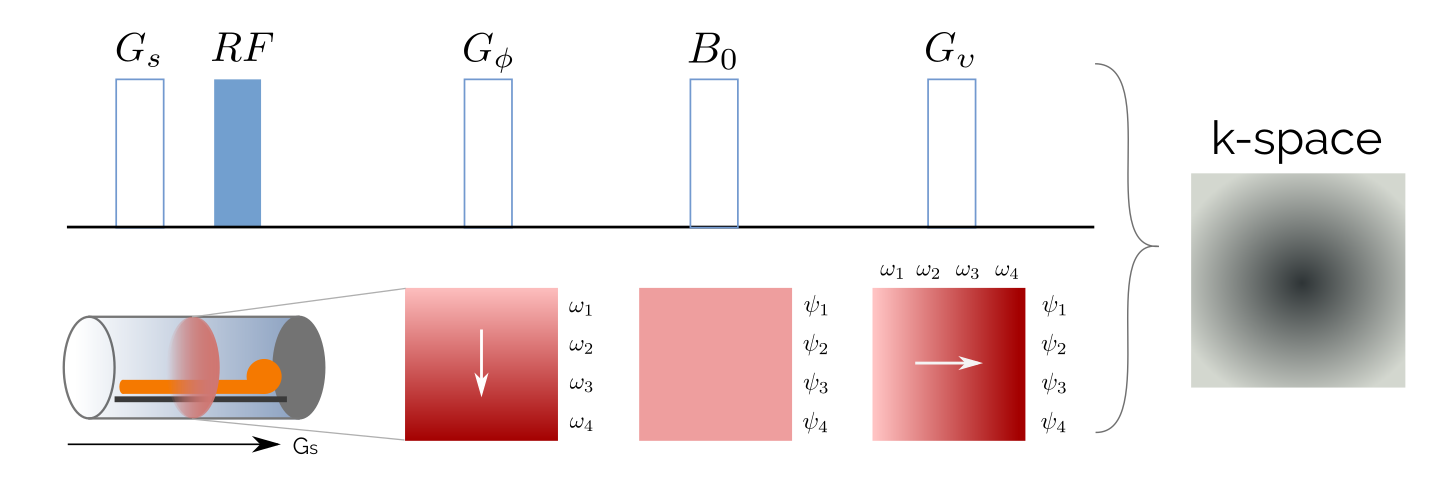
\includegraphics[width=\textwidth]{3.mri/img/kspace.png}
    \caption{Pipeline of a Magnetic Resonance adquisition.}
    \label{fig:kspace}
\end{minipage} ~

\end{figure*}

%In 1946, Bloch \cite{Bloch1946} shows that the variation in Magnetization over time is expressed as:

%$$ \frac{dM(t)}{dt} = \gamma M(t) \times B(t) 
%                      - \frac{M(t) \vec{x} + M(t)\vec{y}}{T_2}
%                      - \frac{(M(t)-M(0))\vec{z}}{T1} $$

%Where $\gamma$ is the gyromagnetic ratio, $B$ is the magnetic field intensity and T1, T2 are relaxation times.

\section{Diffusion Magnetic Resonance Imaging}
The molecules inside a fluid in equilibrium are not still, on the contrary, they are randomly moving around.
This physical phonomena is known as diffusion.
Implications of diffusion in medicine.

In 1956, H.C. Torrey \cite{Torrey1956} observes that the magnetization can be lost by effect of diffusion.
Somebody comes with a new idea of how to measure diffusion by introducing two new gradients.
Let's explain the process in a intuitive way.

Imagine that after applying the RF pulse to do slice selection, we add a gradient field $G_1=G_d$ for a small time $\delta$ms.
As explained in the previous section (sec. X), this will make the protons be off-phase between them.
If after a $\Delta$ time we apply the same gradient, but in the opossite direction $G_2=-G_d$, also for $\delta$ms, then, the protons should go back to be in-phase [fig].
However, the particules undergoing diffusion will have moved (fig.), for which the second gradient $G_2$ would have reach them in a different place, and therefore, change their angular velocity differently.
In this way, a difference in the phase of the protons respect to the rest is a sign of diffusion [fig].
Since a voxel now has protons precessing at different velocities, they create less signal.
Max. signal is achieved when they all rotate together.
The difference between the signal obtained with no diff. gradient and with diff. gradient reflects the amount of diffusion.


\begin{figure}
    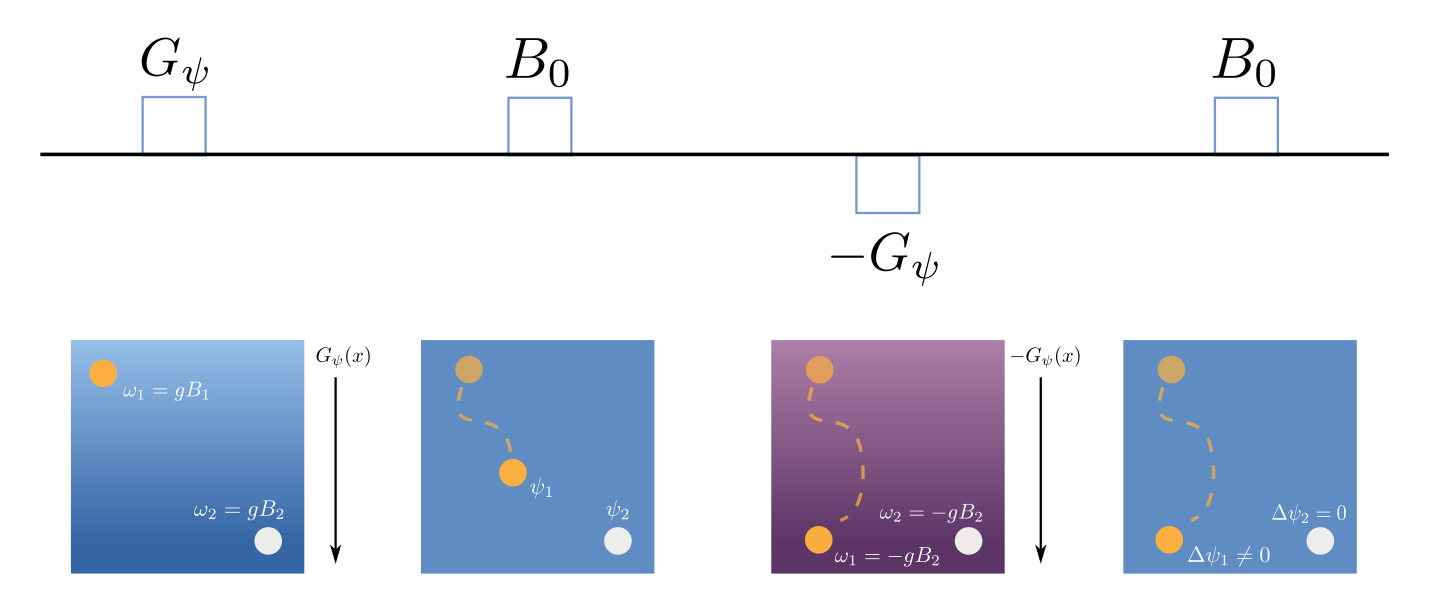
\includegraphics[width=0.49\textwidth]{3.mri/img/dmri.png}
    \caption{Figure explaining dMRI}
    \label{fig:}
\end{figure}  

\subsection{Pulsed Gradient Spin Echo (PGSE)}
\begin{figure}
    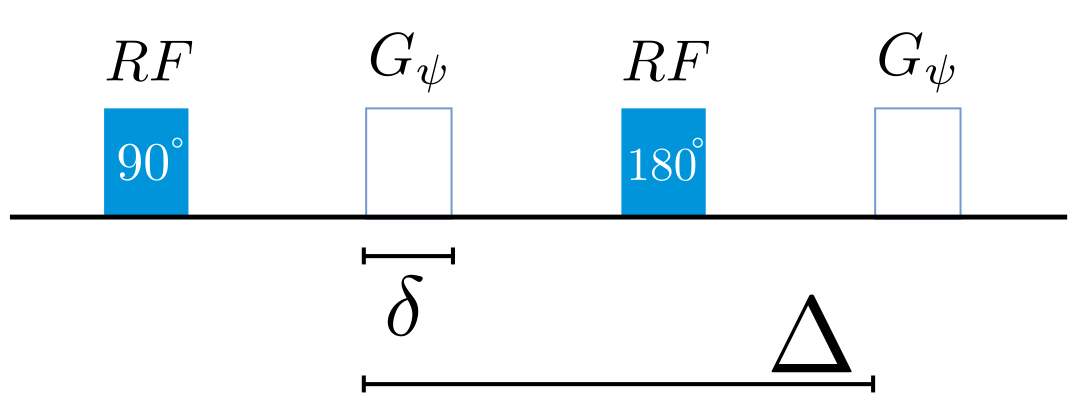
\includegraphics[width=0.49\textwidth]{3.mri/img/fgp.png}
    \caption{Secuencia Pulsed Gradient Spin Echo.}
    \label{fig:fgp}
\end{figure}  

[refrase all]
In 1965, Stejskal and Tanner invent the PGSE sequence to measure diffusion. 
The Stejskal-Tanner imaging sequence [Stejskal and Tanner (1965)] is used to
measure the diffusion of water molecules in a given direction. This pulse
sequence is illustrated in Figure 4.3. This sequence uses two gradient pulses
in the direction g, of duration time δ, to control the diffusion-weighting.
They are placed before and after a 180◦ degrees refocusing pulse.
More specifically, a first 90◦ degrees RF is applied to flip the magnetization
in the transverse plane. The first gradient pulse causes a phase shift of the
spins whose position are now a function of time. Spin position is in fact
assumed to stay constant during time δ. Finally, the 180◦ pulse combined with
the second gradient pulse induces another phase shift. It is applied after a time
∆ separating the two gradient pulses. This pulse cancels the first phase
shift only for static spins. On the other hand, spins under Brownian motion during
the time period ∆ separating the two pulses undergo different phase shifts by
the two gradient pulses, resulting in a T2 signal attenuation [Cercignani and Horsfield. (2001)].
By assuming the pulses to be infinitely narrow (narrow pulse approximation), i.e.
if the gradient pulse duration δ is short enough for the diffusion of the water molecule
to be negligible during that time, [Stejskal and Tanner (1965)] showed that the signal
attenuation S(q,τ) is expressed as the 3-dimensional (3D) Fourier transform
F of the ensemble average propagator P,

[some eq?]

where $E(g, \delta, \Delta)$;
$g$ is the intensity of the gradient field;
$S_0$ is the signal obtained with no diffusion gradient ($g=0 T/m$)
, and $\gamma$ is the gyromagnetic ratio of water.
Notice that we need $S_0$ in the equation, since the diffusion comes from the difference in signal between the 

Assuming the pdf to be gaussian, we get:

\begin{equation}
    E(g, \delta, \Delta) = 
    \frac{S(g, \delta, \Delta)}{S_0} =
         e^{-\gamma^2 g^2 \delta^2 \left(\Delta - \frac{\delta}{3}\right) D} 
    \label{eq:st}
\end{equation}

\subsection{subsection}
In 1985 Le Bihan \cite{LEBIHAN} proposses to gather all the parameters in a single one: 

$$ b = \gamma^2 g^2 \delta^2 \left(\Delta - \frac{\delta}{3}\right) $$ ,

simplifiying the equation \ref{eq:st} to:

$$ E(b) = \frac{S(b)}{S_0} = e^{-b D} $$

where $b$ represents the reciprocal of the diffusion intensity.

In 1994 Basser et al. \cite{Basser1994} propose to measure the signal atenuation in different directions, and then approximate the diffusion coefficient with a second order tensor.
A tensor is a multidimentional matrix associated to a base, which possess a transformation law indicating how the tensor components change when the base change.
This sets the bases of what's known as DTI.
DTI represents the diffusion as a 3-dimentional (3D) elipsoide, which can be coded in a symmetric matrix:

$$
    D =
    \begin{pmatrix}
             D_{xx} & D_{xy} & D_{xz} \\
             D_{xy} & D_{yy} & D_{yz} \\
             D_{xz} & D_{yz} & D_{zz}    
    \end{pmatrix}
$$

Therefore we need at least 6 acquisitions.

One of the main limitants of this method is that it does not allow to
represent the crossing of fibers. They get modeled as spheres.

In 1991 Callaghan et al. \cite{Callaghan1991} developped the q-space analysis.
This allows to make microscopy with dMRI.
Based on the work of Stejskal and Tanner, Callaghan show that it's possible to express the signal attenuation as:

$$E(q,\Delta) =  \frac{S(q,\Delta)}{S_0} = \int_{R^2}{p(r;\Delta)e^{-2\pi i q r} dr} $$
$$ q = \frac{\gamma \delta g}{2\pi} $$

Where $p(r;t)$  is the probability density that a set of particles travels a distance $r$ during a time $t$.
Because of this, $p(r;t)$ is highly related to the compartment where the particles are contained.

One of the main advantages of q-space over DTI is that is does not assume any a prior model, allowing to define different strategies for $p(r;t)$.
Here we talk about \textit{Spherical Harmonics} \cite{Tuch2004} and
\textit{Constrained Spherical Deconvolution} \cite{Tournier2004}, which are the most relevant ones for this thesis.

\section{Tractography}

%TODO
% Explain tractography as a random walk
% Explain its problems
%  Gyral bias
%  Resolution
%  No direction (Jbabdi and Beherens)
%  False positives!!!!!
% Explains that anyway it's the best thing we have

Diffusion in the white matter is constrained by the tracts present on it.
The protons present in any point of the brain will be able to diffuse only inside a tract and along its path.
This means that, by following the diffusion signal, we should be able to trace the brain pathways.
However, most of the methods to model diffusion signal cannot handle correctly the crossing of fibers.
The best we can do, is to derive a probabilistic map from one voxel to another, and simulate the random movement of a water particle from one voxel to another.
We hope that the diffusion signal + some constraints in the random walk allow us to retrieve the real pathways of the brain.
Furthermore, if we generate a big number of this random walks, or streamlines, we hope to be able to recover the underlying tracts in a correct way by means of statistics.
They are some issues with this.
But there are some cool stuff about it also.

[VAN ESSEN]
Using high-resolution postmortem diffusion imaging and tractography in Old World monkeys, we found a correlation coefficient of ~0.58 between tractography-based and tracer- based estimates of connectivity;
the correlation is highest for strong, short-distance pathways but is informative even for weak connections and widely separated areas (Donahue et al., 2016).
We will discuss multiple reasons why tractography imperfectly reflects ground-truth neuroanatomical connectivity.
This includes
(i) a gyral bias in which tractography streamline within ‘gyral blades’ are biased towards gyral crowns rather than sulcal banks (Van Essen et al., 2014);
(ii) an ‘anti-fundus’ bias in which connections to/from sulcal fundi tend to be obscured by tangential fiber bundles immediately subjacent to many sulci (Reveley et al., 2015);
(iii) axonal branching within white matter that includes many branches at approximately right angles (Economo et al., 2016) that are inherently difficult to discriminate from crossing fibers that also occur within white matter;
and (iv) potential dispersion or ‘defasciculation’ in the white matter axonal trajectories of pathways that interconnect widely separated gray matter parcels (Jbabdi et al., 2015).


[MINE]
A primary issue is the spatial resolution of diffusion imaging:
it is several orders of magnitude coarser than axonal diameters (millimeters vs. micrometers) (Van Essen et al., 2014), making hard to infer some brain pathways.
In addition, there is as yet no quantitative measure of the strength of connections from diffusion (Jbabdi and Behrens, 2013).
Given a seed-point in the brain, prob- abilistic tractography creates a tractogram:
an image where each voxel is valued with its probability of being connected to the seed through axonal bundles.
One way of calculating these probabilities is with a Monte Carlo procedure, simulating the random walk of water particles through the white matter (Behrens et al., 2003).
Each one of these paths is known as a streamline.

[MAXIME NATURE NEUROSCIENCE?]
we organized an open international tractography challenge, which resulted in 96 distinct submissions from 20 research groups.
To determine the current state of the art in tractography, we organized  an  international tractography competition and employed a novel validation method based on simulated DWI of a brain‐like geometry.
This ground truth data set represented 25 well‐known valid bundles that covered approximately 70\% of the human brain white matter.

While most state‐of‐the‐art algorithms  reconstructed 90\% of ground truth bundles to at least some extent, on average they produced four times more invalid than valid  bundles. About half of the invalid bundles occurred systematically in the majority of submissions. 
The average ratio of false‐positive to true‐positive bundles was approximately four to one.
This ratio could not be improved by employing higher quality data or even using the gold standard field of local orientations, highlighting that current tractography approaches are fundamentally ill‐posed.


\section{fMRI}
\cite{Glover2011}
All the processes of neural signaling in the brain require energy in the form of adenosine triphosphate (ATP).
When a region of the brain is up-regulated (i.e. activated) by a cognitive task such as finger tapping, the additional neural firing and other increased signaling processes result in a locally increased energy requirement.
The brain respondes by adjusting its blood flow to deliver nutrients such as oxygen and glucose to stressed tissues and allow them to function. Haemodynamic response (HR) allows the rapid delivery of blood to active neuronal tissues.
The second mechanism, termed Blood Oxygenation Level Dependent (BOLD) contrast, was first demonstrated in rats48,50 and later in humans3,37,49,52, and is the contrast that is used in virtually all conventional fMRI experiments. BOLD contrast results from the change in magnetic field surrounding the red blood cells depending on the oxygen state of the hemoglobin. When fully oxygenated, HbO2 is diamagnetic and is magnetically indistinguishable from brain tissue. However, fully deoxygenated Hb has 4 unpaired electrons and is highly paramagnetic59. This paramagnetism results in local gradients in magnetic field whose strength depends on the [Hb] concentration. These endogenous gradients in turn modulate the intra- and extra-vascular blood’s T2 and T2* relaxation times through diffusion and intravoxel dephasing, respectively. Using a gradient refocused echo (GRE) MRI pulse sequence7, the acquisition is made sensitive to T2* and T2. At 1.5T and
3T, the T2* contrast is predominant and is largest in venules61, while at higher field strength the diffusion-weighted contrast of T2 relaxation becomes more important and, because signals are generated preferentially in capillaries and tissue with spin-echo acquisitions, provides greater spatial specificity57,64. Since most fMRI is currently performed at 3 Tesla or below, BOLD fMRI utilizes primarily GRE methods because of the increased T2* contrast10.

[wikipedia et al.]
Cerebral blood flow (CBF) is the blood supply to the brain in a given period of time.[     Tolias C and Sgouros S. 2006. "Initial Evaluation and Management of CNS Injury."]
The most common functional imaging signal is the blood-oxygen-level dependent signal (BOLD), which primarily corresponds to the concentration of deoxyhemoglobin.[12] The BOLD effect is based on the fact that when neuronal activity is increased in one part of the brain, there is also an increased amount of cerebral blood flow to that area which is the basis of haemodynamic response. This increase in blood flow produces an increase in the ratio of oxygenated hemoglobin relative to deoxygenated hemoglobin in that specific area. The difference in magnetic properties of oxygenated and deoxygenated hemoglobin is what allows fMRI imaging to produce an effective map of which neurons are active and which are not. In short, deoxygenated hemoglobin is paramagnetic while oxygenated hemoglobin is diamagnetic. Diamagnetic blood (oxyhemoglobin) interferes with the magnetic resonance (MR) signal less and this leads to an improved MR signal in that area of increased neuronal activity. However, Paramagnetic blood (deoxyhemoglobin) makes the local magnetic field inhomogenous. This has the effect of dephasing the signal emitted in this domain, causing destructive interference in the observed MR signal. Therefore, greater amounts of deoxyhemoglobin lead to less signal. Neuronal activity ultimately leads to an increase in local MR signaling corresponding to a decrease in the concentration of deoxyhemoglobin.[13]

\section{Conclusion}
This chapter introduced the imaging techniques of MRI, Diffusion MRI and
Functional MRI. These three methods provide means to study the brain anatomy,
structure and function in a non-invasive way. Even when each technique has its
own limitations, either in spatial or temporal resolution, they all allowed to
highly advance the state of the art in neuroscience. In the next chapter we
will see how these advances in imaging allowed to parcellate the brain, making
it easier to study brain function.

\chapterbib

    \chapter{Mapping the Brain: A review of the brain divisions}

\section{Overview}
The brain is composed of billions of neurons interacting at the same time
between them. Given the complexity of this network, a dimensionality reduction
is needed in order to study its properties. Since its beginning, neuroscientist
have divided the brain based on different criteria. This allows to study the
brain as a set of interacting regions, allowing to abstract the underlying
neuronal complexity. However, it's not clear that a unique and truth division
of the human brain exists. In this chapter, we make a review of the different
type of parcellations that exist; explain their advantages, and the best
scenarios where to use each.

\section{Introduction}
Composed by billions of interconnected neurons, the brain is the most complex
biological machine that we know. Untangling this network is of special importance
to understand the underlying process of concious life. However, studying the 
brain at the cellular level, alongside their interactions is simply not feasible.
Existent techniques to study brain microstructure are highly invasive, and can
only be used in postmortem tissue [cite]. Furthermore, while this techniques
succefully help to characterize the cellular composition of the tissue, they
do not allow to account for the interaction between cells. Specially for whole
brain data, the obtained dataset are simply too huge to be handled [cite].
Because of all of this, some way to reduce dimentionallity is needed.

Thanks to the study of cythoarquitectonics, brain function, and tracers we know
that neighboring neurons tend to work together [many cites]. In particular,
the brain behaves as a small world graph. While which populations
of neurons, and how they interact between is highly subject dependant, this
studies give us a solid support to subdivide the brain before studying it.
Nowadays, subdividing the brain in regions homogeneous respect to some criteria
is a necessary first step of every study in neuroscience. By doing so, it's not
only possible to reduce the dimensionality of the network, but also to derive
rules more general than in the cellular case. Furthermore, having consistent
divisions across subjects allows to infer properties from a population. The 
problem recides in the fact that there's not a gold standard/unique division of
the human brain. How to divide the brain will heavily depend on the task desired
to achieve, since using the wrong parcellation can introduce a bias in the
results. 

Historically, the brain has been divided following different criteria. Furthermore,
with every new technological advance, new parcellations arise. Perhaps the first
parcellation to exist was the anatomical one. Still something from Demians thesis
here. Based solely in the brain morphology, gross divisions of the brain can be
made, as lobes and etc. Then, through the study of brain lesions, brain surgery
and EEG allowed to study brain function, from which gross functional divisions
arise. A couple of years later, Brodmann creates his map based on the
cythoarchitecture. Enter MRI to improve anatomical divisions, PET/fMRI for functional
and more recently dMRI for structural. Then, semantical, and finally, the
multischeme ones.

In this chapter, we make a review of the most important techniques of which
we know about for each modality, giving a brief introduction to how they work
and their main strenghts. All the reviewed parcellations are comprised in the
table X. The chapter is divided in the following: Introduction, Parcellations
and Discussion.

Speciall issue neuroimage \cite{The2018}1

\section{Anatomical}
The regions on an Anatomical divisions of the brain are defined by their shape
or relative position in the brain. For example, in the Desikan atlas, the
pars opercularis region is defined as 'the first gyrus from the precentral gyrus'.
The division of the brain in lobes is a coarse anatomical parcellation, finer
divisions can be created based on the sulci. AAL\cite{Landeau2002} is the most used anatomical
atlases. It divides the brain in 45 anatomical volumes of interest. It was
created by manual parcellation of the spatially normalized single-subject 
high-resolution T1 volume provided by the Montreal Neurological Institute (MNI) \cite{Collins1998}.
One of the most used anatomical atlases is that of Desikan~\cite{Desikan2006}.
Another anatomical atlas is the Harvard-Oxford cortical/subcortical atlases,
distributed with the software FSL [CITE].
The desikan atlas divides each hemisphere in 34 coarse structures (Fig X), and each
area is delimited mostly by sulcus. Desikan atlas is built on the cortical surface by: projecting the cortical folding
patters into a spherical surface, aligning them with an atlas computed from the
average of 40 subjects, and then transfering the labels from the atlas to the
cortical surface. Another one, Destrieux, divides the brain in 74 labels per
hemisphere. The labeling is done following a probabilistic model that takes
into account informationas: curvature and average convexity of the cortica
surface, prior labeling probability for that vertex, as well as the labels
of vertices in a local neighborhood.

add MarsAtlas

https://biomedia.doc.ic.ac.uk/brain-parcellation-survey/


\section{Cythoarquitecture}
\label{sec:cyto_maps}
Only the borders of a few architectonically defined areas show a sufficiently precise association with sulci~\cite{Amunts2007}
As shown with modern techniques, borders between cytoarchitectonic areas are functionally relevant, to the point that many functional regions are refered using cythoarquitectonic labels.

Cythoarquitectonic divisions of the brain are based solely in the cellular
composition of the cortex. In this atlases, a brain region possess a consistent
thickness and cellular organization. For example, Brodmann Area 4 has an unusually
thick cortex; possess giant pyramidal cells, and lacks an internal and external
granular layer. The pioneers in the area are Meynert [CITE4-Thiarhou],
Campbell [CITE5] who divided the cortex into 14 areas, and Elliot Smith [CITE6]
into 50.

The most known cythoarchitectonic division of the brain is that
of Broadmann~\cite{Brodmann1909}. Broadmann defines 52 cortical regions, based
on the inspection trough microscope of cortical sections on post-mortem
primates brains. In 1925 von Economo and Koskinas publish the 'Atlas of 
Cytoarchitectonics of the Adult Human Cerebral Cortex' [CITE]. Economo and
Koskinas [cite] recognized 54 fundamental cytoarchitectonic areas with 76
variants and 107 modifications~\cite{Triarhou2007}. Their atlas is based in the
examination of mentally healthy subjects in the range of 30–40 years of age
through improved microscopes. We also have the Jubrain~\cite{Mohlberg2012}, a
cytoarchitectonic probabilistic maps viever, made by Juelich and Duesseldorf
institutes by analizing the histological sections of ten human postmortem brains.
More recent work includes the study of
neurotransmitter receptors to map divisions in the visual cortex~\cite{Eickhoff2008}, 
and the introduction of microstructural metrics, as the gray level index
[CITE](Schleicher and Zilles, 1990), to create observer-independent parcellation
methods, 

Creates an atlas of the human ventral visual stream from the postmortem brain
of 11 subjects\cite{Rosenke2018}.
    
Extant cytoarchitectonic maps do not cover the complete cerebral cortex. 
Only approximately 40\% of the cortical surface has been mapped up to now. 
This is caused by the difficulties of: studying sections; 3D reconstructing the
histological sections, and registration of post-mortem data to a reference space.
This is a very time-consuming process, requiring as minimum as 1 person year for
an area.


\section{Functional}
Functional parcellations of the brain denotes how different human functions 
are localized in the brain. This is, each region is in charge of a specific
function (i.e. movement, speach, vision), or is part of a greater system with
a specific functional or cognitive goal. The first functional maps where derived
from lessions. A classical example is that of Broca and Wenicke areas, related
to meaningfull speach production and spech comprehension. The areas are named
after Broca [CITE] and Wernicke [CITE], who in the late 1800 reported lesions in
that region for aphasic patients. Another example is the human homunculus,
a representation of motor and sensory functions, which Penfied [cite] mapped
trough experimenting with electrical stimulation of different brain areas of
patients undergoing open brain surgery.

As stated in the previous section (sec. \ref{sec:cytho_maps}, Cythoarchitectonic
parcellations can be seen as functional ones, since they show close relation 
to function. However, they do not cover the whole brain, and we can only relate
them after many patients show specific impediments and have lesions in those
regions. The advenment of functional MRI (fMRI) allowed to measure the level of
oxygen in blood. Knowing that the neurons need oxygen as fuel to fire, we can
find wich region of the brain are being activated for specific tasks. This
allowed to refine and validate in vivo the functional specialization of 
cythoarchitectural parcels and to better define anatomical ones as the human
humunculus \cite{Lashkari2010, Michel2011}. Even more interesting is the fact
that there are some regions that activate while in a resting state. From the
no-task state (resting state), is possible to derive parcellations by seing
which systems activate simultaneusly. The most common way is to computed the
Pearson's correlation between the fMRI time series at each spatial location.
While we have no idea what this means, people uses it. 

PNAS of 2004 \cite{Johansen-Berg2004}


%\cite{Power2012} use Graph analysis and subgraph detection techniques in order
%to characterize functional subnetworks in the connectivity graph. 
Yeo et al. [CITE] 
Data from 1,000 subjects were registered using surface-based alignment.
The connectivity fingerprints were modeled with a von Mises-Fisher distribution,
then, the data points were randomly assigned to different groups and then
iteratively reassigning the group memberships of points to maximize the
agreement of connectivity profiles among points of the same group. The results
yield a 7 parcels and 17 parcels network.

The Cortical Area Parcellation from Resting-State Correlations dataset consists
of 333 cortical patches segmented using resting-state fMRI (Gordon 2014).

By applying different clustering algorithms to this matrix, we
obtain different parcellations. We can use ward clustering [cites from Thirion];
k-means clustering [cites from thirion]; spectral clustering [cites from thirion],
and principal component analysis (PCA) [cites from thirion]. There are also
local gradient approaches, that detect abrupt transitions in functional
connectivity patterns \cite{Wig2014, Schaefer2017}. 
Based on the work by Thomas Yeo et al. [CITE], Schaefer et al.  \cite{Schaefer2017}
add further refinement by subparcellating the global networks based on a local
gradient approach. Parcellations come in several version, breaking down the cortex
into up to 1000 regions based on rs-fMRI.

Presents a multigraph K-way clustering method and applies it to obtain 
parcellations of 50, 100, 150... maybe put in the same bag as the rest \cite{Shen2013}.


A fine-grained parcellations ranging form 200 to 1000 parcellations,
using spectral clustering on rs-fMRI connectivity matrix \cite{Craddock2011}.

Thomas Blumensath et al. makes a thousand small functionally homogeneous regions,
and then apply hierarchical clustering to obtain the rest of the parcellations \cite{Blumensath2013}.

Huth et al. atlas \cite{Huth2016} maps semantic selectivity across the cortex
by using voxel-wise modelling of functional MRI (fMRI) data collected while 
subjects listened to hours of narrative stories. This creates a map where each
region is ligated to a specific systematically map semantic domain. In this
maps, a region of the brain is ligated to a specific semantic domain, i.e.
violent, temporal, proffesional \cite{Huth2016}.

While we dont do EEG, you can review it here \cite{Shen2013}.

add \cite{Ryali2013} https://www.ncbi.nlm.nih.gov/pubmed/23041530

%Good review in:
%https://www.biorxiv.org/content/biorxiv/early/2017/06/06/135632.full.pdf
%https://biomedia.doc.ic.ac.uk/brain-parcellation-survey/


\section{Structural Connectivity}
In a structural parcellation, regions have a homogeneous pattern of connectivity
with the rest of the brain. This is, a region is defined as: 'all of the points
inside are connected to some other ROIs in a similar way'. The granularity
of the ROIs can go from coarse brain regions, defined by other atlas, to voxels.
The first connectivity divisions came form tracers in monkey PANDIAS. Diffusion
MRI (dMRI) enables the in vivo exploration of extrinsic connectivity on the
human brain. As with fMRI, the most common way to generate a parcellation is
to compute a connectivity matrix, and then parcellate it using some clustering
technique. Given the difficulty of handling huge connectivity matrices, initial
techniques used to divide only portions of the brain.

Behrens et al.\cite{Behrens2003} thalamus Hard segmentation was performed by classifying the seed voxel as connecting to the cortical mask with the highest con- nection probability.
Alfred Anwander performs k-means\cite{Anwander2006} in the connectivity matrix of Broca's area.
Thiebaut de Schotten et al. divide the occipital cortex\cite{ThiebautdeSchotten2014}, frontal lobe \cite{ThiebautdeSchotten2016}
Moreno-Dominguez et al. use a constrained hierarchical clustering to parcellate a structural matrix \cite{Moreno-Dominguez2014}
Gallardo buils on top of this.
They use spectral reordering to study the organization of the temporal lobe \cite{Bajada2017}
(O'Muircheartaigh and Jbabdi, 2017) is entirely data-driven (based on independent component analysis) and allows one to obtain sets of white matter components with their associated gray matter networks \cite{Muircheartaigh2018}


Previous single-subject structural parcelling techniques work by refining other
parcellations~\cite{Clarkson2010};parcelling only part of the
cortex~\cite{Lefranc2016, Roca2009, ThiebautdeSchotten2014, ThiebautdeSchotten2016},
perform a groupwise parcellation after constructing an average connectivity profile~\cite{Clarkson2010, Roca2010},

Parisot uses ideas from cosegmentation and spectral decomposition to create consistent groupwise parcellations \cite{Paristot2015}.


\section{Multi-modal}
So far, all the presented methodologies were solely on one technique. In
multi-modal parcellations, the goal is to mix two or more 
Parisot \cite{Parisot2017}.
Based on function, Van Essen \cite{Glasser2016}.
Braintome\cite{Fan2016}
Structural+Functional correlation and then hierarchical clustering\cite{Diez2014}


\section{Discussion}
The brain atlas concordance problem: quantitative comparison of anatomical parcellations.

Here we name them, some people profile them:

Thirion did it for functionali \cite{Thirion2014}
Arslan did it for functional \cite{Arslan2018}
Gorgolewski KJ, Tambini A, Durnez J et al. Evaluation of full brain parcellation schemes using the NeuroVault database of statistical maps [version 1; not peer reviewed]. F1000Research 2017, 6:1986 (poster) (doi: 10.7490/f1000research.1115065.1) 

Some other reviews: Jbabdi \cite{Jbabdi2013}, \cite{Arslan2018}, 

Gatherings: http://www.lead-dbs.org/helpsupport/knowledge-base/atlasesresources/cortical-atlas-parcellations-mni-space


There's not such a thing as a unique brain parcellation. While we cannot say
that it doesn't exist. We know that all of our techniques have a limitation,
either in resolution, SNR. At the same time, we cannot study things at the
neuron level, because we have billions of neurons in the brain. It makes a
lot of sense that each parcellation is different, because they're based
in different criteria. Even when trying to parcellate data coming from a
same machine (fmri, dmri, etc), changing the hypothesis will change the 
resulting parcellation. For example, in structural gradient vs structural
parcel. The important thing is to be able to select the right parcellation
for the right study.

The important thing is to validate it correctly, some people do, like \cite{Gallardo}, \cite{Auzias2016}, \cite{ThiebautdeSchotten2014, ThiebautdeSchotten2016}

\section{Resume of all of the parcellations presented}
Here I put a beautiful table resuming everything.

\section{Conclusion}
In order to reduce the complexity of the brain many studies start by subdividing
the brain. Depending on the hypothesis driving the study, different type
of parcellations can be used. In this chapter we presented parcellations based
on different criteria: cythoarquitecture; anatomy, function, semantics and
structural. We also presented some parcellation which are driven by a mixture
of suche criteria. Each parcellation possess its own advantages, and should be
used in the right context. In the following chapter we will introduce the
first contribution of this thesis: a technique to parcellate the cortex based
on its structural connectivity. Our technique allows to create parcellations
at the single-subject and group level, while having a good correlation with
known divisions of the brain.


\chapterbib

    \chapter{Groupwise Structural Parcellation of the Whole Cortex: A Logistic Random Effects Model Based Approach}
%
%
\section{Overview}
So far in this thesis we have introduced the necessary concepts in neuroanatomy;
non-invasive imaging techniques to study the brain, and brain parcellation. In
the first chapter we explained the importance of brain connectivity and its
relation to brain function. On the second chapter, we explained how to estimate
brain connectivity and brain function in a non-invasive way. The third chapter
showed the ongoing effort to find new and relevant ways to divide the brain,
in order to improve the way to study it. In particular, all of the parcellations
based on structural connectivity are computationally expensive; need tuning of
several parameters or rely on ad-hoc constraints. Furthermore, none of these 
methods present a model for the cortical extrinsic connectivity of the cortex.
In this chapter, we propose a parsimonious model for the extrinsic connectivity
and an efficient parceling technique based on clustering of tractograms. 
Our technique allows the creation of single subject and groupwise parcellations
of the whole cortex. We show that our technique creates parcellations in
agreement with anatomical, structural and functional parcellations extant in 
the literature.

This work has been published in the journal Neuroimage \cite{Gallardo2017}
%
\section{Introduction}
%
The human brain is arranged in areas based on criteria such as cytoarchitecture,
functional specialization or axonal connectivity~\citep{Brodmann1909, Thirion2014,
ThiebautdeSchotten2016}. Parceling the cortex into such areas and 
characterizing their interaction is key to understanding how the brain works.
Nowadays it is accepted that axonal connectivity plays a fundamental role in the
interaction between brain regions~\citep{Schmahmann2006}. Moreover, current theories
hold that long-range physical connections trough axonal bundles,
namely \textit{extrinsic connectivity}, are strongly related to brain function, for example,
this has been shown in macaques~\citep{Passingham2002}. Therefore, understanding
how the cortex is arranged based on its extrinsic connectivity can
provide key information in unraveling the internal organization of the brain.

Diffusion MRI (dMRI) enables the in vivo exploration of extrinsic connectivity 
and other aspects of white matter anatomy on the brain. However, in using diffusion
MRI to infer long-distance connectivity, several challenges arise. A primary issue
is the spatial resolution of diffusion imaging: it is several
orders of magnitude coarser than axonal diameters (millimeters vs.
micrometers)~\citep{VanEssen2014}, making hard to infer some brain pathways.
In addition, there is as yet no quantitative
measure of the strength of connections from diffusion~\citep{Jbabdi2013}.
Given these general limitations, obtaining a cortical parcellation based on
extrinsic connectivity remains challenging~\citep{VanEssen2014, Jbabdi2013}.
Moreover, most current parceling
techniques compute either single-subject or groupwise parcellations.
Single-subject techniques work by refining other
parcellations~\citep{Clarkson2010}, which introduces a bias in the resulting
parcellation; parceling only part of the 
cortex~\citep{Lefranc2016, Roca2009, ThiebautdeSchotten2014, ThiebautdeSchotten2016}
or using ad-hoc metrics to compare extrinsic connectivity~\citep{Moreno-Dominguez2014}.
Meanwhile, existing groupwise methods rely on average connectivity
profiles~\citep{Clarkson2010, Roca2010}, which prevents obtaining single
subject parcellations; seek a matching across subjects after independent
parcellations~\citep{Moreno-Dominguez2014}, relying on possible noisy results,
or need fine tuning of parameters, as the expected number of clusters to
find~\citep{Paristot2015}.

\begin{figure*}
    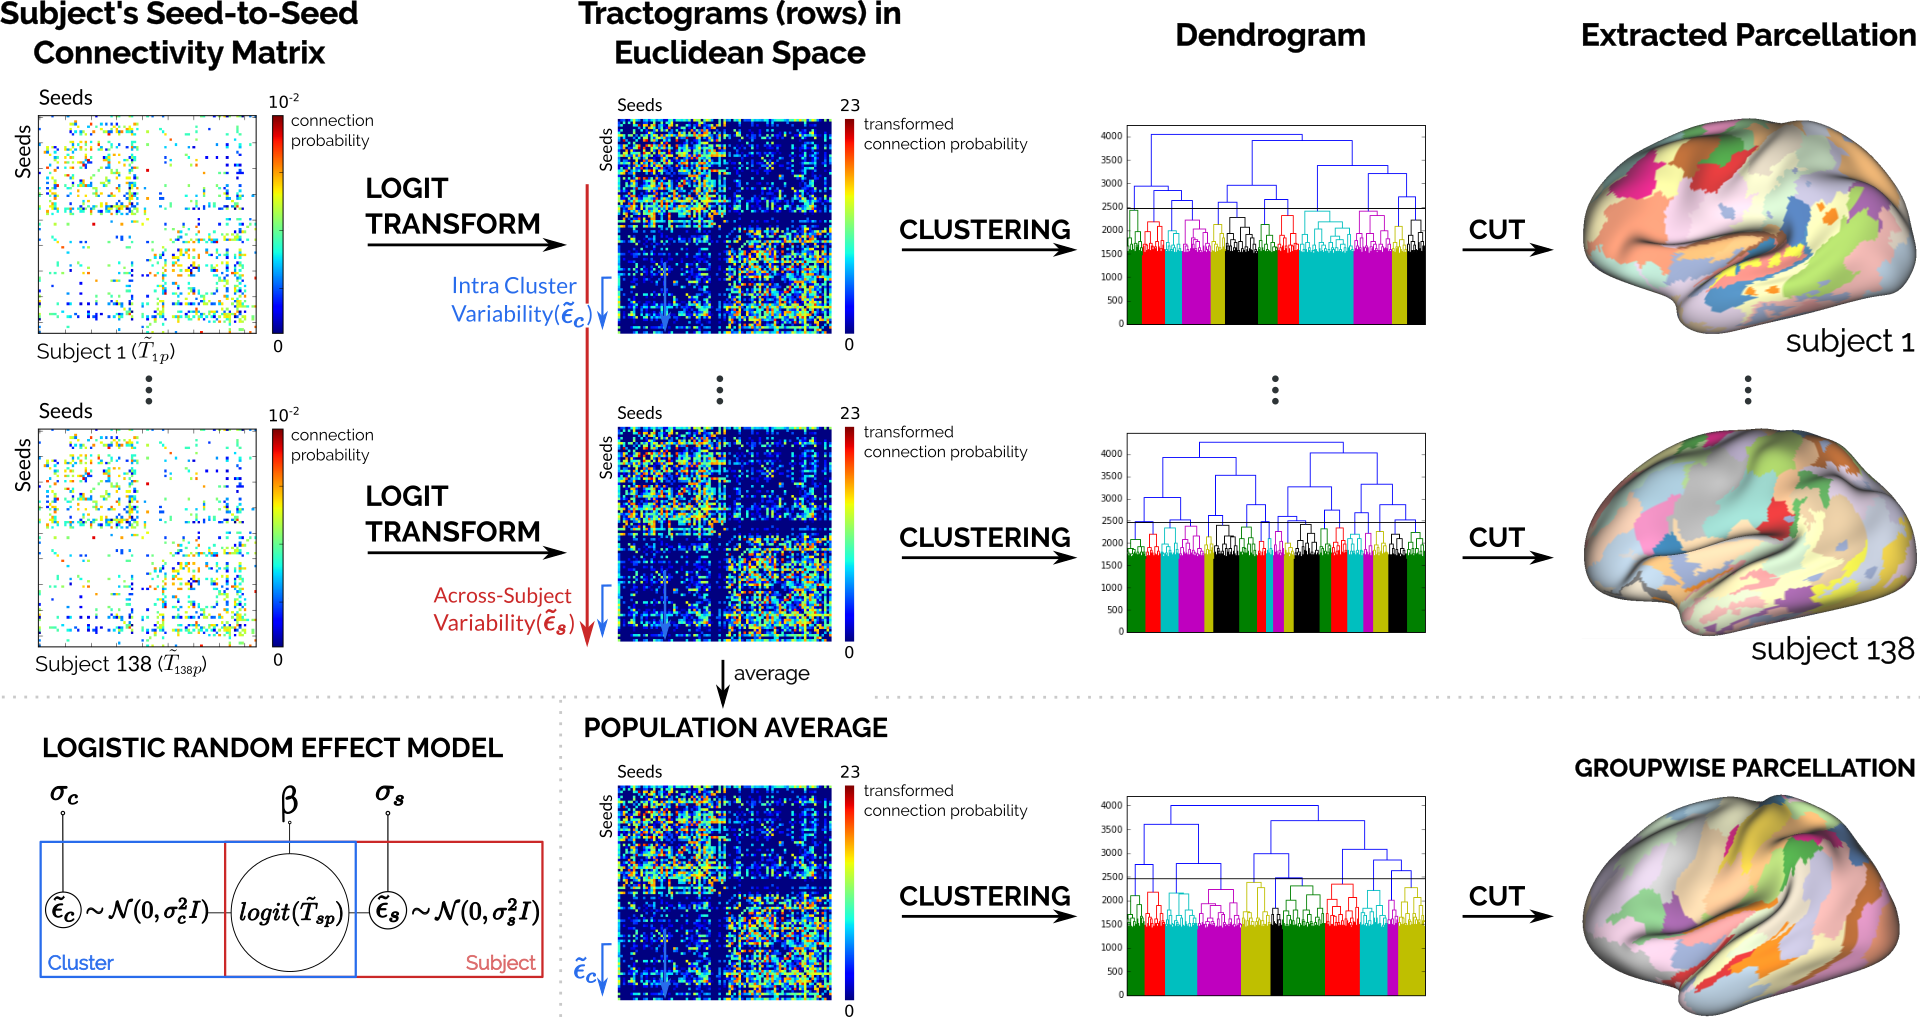
\includegraphics[width=\textwidth]{5.structural_clustering/img/summary.png}
    \caption{Lower left corner: graphical model of the linear relationship
             between the tractogram of a subject $s$ for a seed $p$ ($\tilde T_{sp}$); and the intra-cluster
             ($\tilde \epsilon_c$) and across-subject ($\tilde \epsilon_s$) variability of the seed's patch. We transform the tractograms 
             into a Euclidean space while explicitly accounting for the variability. This allows us to use well known clustering techniques and 
             compress different levels of granularities for a same parcellation
             in a dendrogram.}
    \label{fig:summary}
\end{figure*}

In this work, we present a parsimonious model for the cortical
connectivity alongside an efficient parceling technique based on it. We summarize
both contributions in Fig.~\ref{fig:summary}. Our model assumes that the cortex is
divided in patches of homogeneous extrinsic connectivity. That is, nearby
neurons in the cortex share approximately the same long-range physical
connections, we call this the \textit{local coherence criterion}. Our assumption
is based on histological results in the macaque brain~\citep{Schmahmann2006}.
Inspired by statistical models for clustered data~\citep{Pendergast1996}, our model
accounts for the variability in the axonal connections of neurons within a patch
and for variability in patch boundaries across subjects. Our parceling technique
allows us to create single subject and groupwise parcellations of the whole
cortex in agreement with extant parcellations.

We validate our technique by taking advantage of data available from the Human
Connectome Project (HCP). Using our technique, we compute single subject and a
groupwise parcellations. In this work we will focus on the groupwise case. For
results of our method on the single-subject case please refer to \citet{Gallardo2017}.
Here, we first assess the consistency of our groupwise parceling technique by
comparing the groupwise parcellations of three disjoint groups of 46 subjects
from the HCP. We also show that our technique computes a similar parcellation to
the one obtained by \citet{ThiebautdeSchotten2016} when parceling only the frontal
cortex. Later, to test the functional specialization of our frontal lobe parcels,
we use a data-base of meta-analysis of fMRI studies \citep{Yarkoni2011}, as in
\citet{ThiebautdeSchotten2016}. After, we show that our groupwise parcels subdivide
some well-known anatomical structures by comparing our results against Desikan's
atlas~\citep{Desikan2006}. Also, we show the functional specialization of some of
our parcels by comparing against results from \citet{Glasser2013}. Finally, we
compare our groupwise parcellation of 138 subjects against the multi-modal
parcellation of \citet{Glasser2016}. We show that, while the parcellations
boundaries differ, our parcels show similar or better functional specialization,
specially for motor related tasks.

This work is organized as follows: In the Methods section we present our
model for cortical connectivity and frame tractography within our model. Also,
we present both our single-subject and groupwise case methodologies to parcellate
the cortex. In the Experiments and Results section we present our results on HCP
data. We then discuss our results and position ourselves with respect to the state
of the art in the Discussion section. Finally, in the last section we provide our
conclusions.
%
\section{Methods}
%
\subsection{Cortical Connectivity Model and Tractography}
\label{sec:cortical_model}
Our model assumes that the cortex is divided in clusters of homogeneous extrinsic
connectivity. That is, nearby neurons in the cortex share approximately the same
long-ranged physical connections, we call this the \textit{local coherence criterion}.
Our assumption is based on histological results in the macaque brain~\citep{Schmahmann2006}.
As in clustered data models in statistics~\citep{Pendergast1996}, we allow
intra-cluster and across-subject variability in the connectivity. We formalize this concept as:
%
\begin{equation}
    \label{eq:notation}
    K = \bigcup_{i=1}^k K_i , \forall_{1 \leq i,j \leq k}, i \neq j \rightarrow K_i \cap K_j = \emptyset \land \on{conn}(K_i) \neq \on{conn}(K_j)
\end{equation}
%
where the set of points on the cortex $K$ is the disjoint union
of each cluster $K_i$ and $\on{conn}(\cdot)$ is the extrinsic connectivity
fingerprint of a cluster. We will make the notion of variability explicit in eq. 
\ref{eq:tractogram_rv}. In this work, the connectivity fingerprint of a seed-point
in the brain is a binary vector denoting to which other seed-points it is
connected through axonal bundles. That is, the physical connections of a point
$p \in K_i$ in the brain are represented by its connectivity fingerprint
$\on{conn}(p) = \on{conn}(K_i)$.

Currently, the most common tool for estimating the extrinsic connectivity
fingerprint of a point in vivo is probabilistic tractography~\citep{Jbabdi2013}.
Given a seed-point in the brain, probabilistic tractography creates a
\textit{tractogram}: an image where each voxel is valued with its probability
of being connected to the seed through axonal bundles. One way of calculating
these probabilities is with a Monte Carlo procedure, simulating the random walk
of water particles through the white matter~\citep{Behrens2003a}. Each one of
these paths is known as a streamline. If we model these streamlines as Bernoulli
trials, where we get a value for the connection from our seed with other points
(1 if they connected by the streamline, 0 if not)~\citep{Behrens2003a}, then, we
can model the tractogram of the subject $s$ in the seed-point $p$ as:
%
\begin{equation}
    \label{eq:tractogram}
    T_{sp} = 
      [P(\rv C_{spi}=1)]_{1 \leq i \leq n} =
      [\theta_{spi}]_{1 \leq i \leq n}, ~~ \rv C_{spi} \sim \on{Bernoulli}(\theta_{spi})
    \enspace,
\end{equation}
%
where $\rv C_{spi}$ is a Bernoulli random variable\footnote{For the sake of
clarity we denote all random variables with a tilde, e.g. $\rv C$.} 
representing ``the point $p$ of the subject $s$ is connected to the voxel $i$".
Each Bernoulli's parameter ($\theta_{spi}$) represents the probability of being
connected, and is estimated as the proportion of success in the Bernoulli
trials of each seed.

To formulate the tractogram in accordance to our hypothesis of cortical
connectivity, we model it as a vector of random variables. In our
model, each element in a tractogram comes from a random variable depending on
the point's cluster along with its intra-cluster and across-subject variability:
\begin{equation}
    \label{eq:tractogram_rv}
        p \in K_c \rightarrow
        \rv T_{sp} = 
        [P(\rv C_{spi}=1 | \on{conn}(K_c), ~\rv \epsilon_{ci}, ~\rv \epsilon_{si})]_{1 \leq i \leq n}
        \enspace ,
\end{equation}
%
in this case, the point $p$ belongs to the cluster $c$;  $\rv \epsilon_{ci}$ 
represents the intra-cluster variability and $\rv \epsilon_{si}$ represents the
across-subject variability for the connectivity to voxel $i$ in the cluster $c$. 

Since each $\rv C_{spi}$ follows a Bernoulli distribution (Eq. \ref{eq:tractogram})
it is difficult to find an explicit formulation for 
$P(\rv C_{spi} = 1 | \on{conn}(K_c),~\rv \epsilon_{ci}, ~\rv \epsilon_{si})$ 
accounting for the variabilities. For this, we use the generalized linear
model (GLM) theory. In this theory, the data is assumed to follow a linear form
after being transformed with an appropriate link function~\citep{McCullagh1989}.
Using the following notation abuse:
%
\begin{equation}
    \label{eq:not_abuse}
    \on{logit}(\rv T_{sp}) \triangleq  [\on{logit}(P(\rv C_{spi}=1 | \on{conn}(K_c), ~\rv \epsilon_{ci}, ~\rv \epsilon_{si})]_{1  \leq i \leq n},
\end{equation}
\noindent
%
we derive from GLM a logistic random-effects model~\citep{Pendergast1996} for
each point $p$:
%
\begin{equation}
    \label{eq:ran_eff_model}
    \on{logit}(\rv T_{sp}) = \beta_{c} + \rv \epsilon_{c} + \rv \epsilon_{s} \in \R^n,
    \quad
    ~ \rv \epsilon_{c} \sim \N(\vec 0, \sigma_c^2 Id),
    ~ \rv \epsilon_{s} \sim \N(\vec 0, \sigma_s^2 Id),
\end{equation}
%
where $\epsilon_{c}$ and $\epsilon_{s}$ represent the intra-cluster and 
across-subject variability respectively. According to GLM theory 
$\beta_c \in \R^n$ is the extrinsic connectivity fingerprint of cluster $K_c$
transformed: 
%
\begin{equation}
    \on{logit}^{-1}(\beta_c) = E(\rv T_{sp}) = \on{conn}(K_c) \enspace.
\end{equation}

The choice of logit as link function is based on the work of \citet{Pohl2007}.
In their work, \citet{Pohl2007} show that logit function's codomain is a
Euclidean space, which allows us to transform and manipulate the tractograms 
in a well-known space.
%
\subsection{Single Subject and Groupwise Parceling Methodologies}
\label{sec:parceling_methodologies}
%
In the previous section, we hypothesized that the cortex is divided in
clusters with homogeneous extrinsic connectivity, alongside intra-cluster and
across-subject variability. In using
the previous hypothesis, it is important to remark that we don't have a priori
knowledge of the cluster's location or their variability. But, thanks to the
proposed logistic random effects model, we formulated the problem of finding
these clusters as a well-known clustering problem. This is because, after
transforming the tractograms with the logit function as in eq.~\ref{eq:not_abuse}
they will be in a Euclidean space~\citep{Pohl2007}. Even more, eq.~\ref{eq:ran_eff_model}
states that the transformed tractograms come from a mixture of Gaussian 
distributions, e.g. it is a Gaussian mixture model.

To solve the Gaussian mixture model and find the clusters, we use a modified
Agglomerative Hierarchical Clustering (AHC) algorithm. This was inspired by the
method of \citet{Moreno-Dominguez2014}. To enforce the local coherence
criterion we also modify the algorithm to accept one parameter: the minimum size
of the resulting clusters. Clusters smaller than this size are merged with
neighbors, i.e. physically close clusters in the cortex. As we are working in
a Euclidean space, we use Ward's Hierarchical Clustering
method~\citep{WardJr.1963}. 
This method creates clusters with minimum within-cluster variance.
The method's result is a dendrogram: a structure that comprises different levels of
granularity for the same parcellation. This allows us to explore different
parcellation granularities by choosing cutting criteria, without the need of
recomputing each time.

The main advantage of the model we proposed in this work is that it
allows us to create a groupwise parcellation using linear operations. Assuming
direct seed correspondence across subjects, as in the HCP data set, our model
lets us remove the subject variability of each seed's tractogram by calculating
the expected value across subjects:
%
\begin{equation}
    \label{eq:expected_subject}
    E_s(g(\rv T_{sp})) = E_s(\beta_{c} + \rv \epsilon_{c} + \rv \epsilon_{s}),
    = \beta_{c} + \rv \epsilon_{c} + E_s(\rv \epsilon_{s})
    = \beta_{c} + \rv \epsilon_{c}.
\end{equation}
% 
where the last equality is due to $E_s(\rv \epsilon_s)=0$
(Eq. \ref{eq:ran_eff_model}). Since in our model the variabilities are normally
distributed (Eq. \ref{eq:ran_eff_model}), we can estimate the expected value across
subjects by averaging a seed's tractograms across subjects. This allows us to create
population-representative tractograms for each seed free of across-subject 
variability, which then can be clustered to create a groupwise parcellation.
%
\section{Experiments and Results}
%
In the previous section we presented a model for the cortical extrinsic 
connectivity and a clustering technique to parcellate the whole brain. Our technique
allows us to create single subject and groupwise parcellations, encoded with
different levels of granularity in a dendrogram. Now, we show the results of
applying our technique over the HCP dataset. First, we explain how the 
preprocessing step of tractography was made. Then, we elaborate 
in detail how we applied our technique. Later, we show that our groupwise 
technique creates results consistent when parceling different groups. Also,
we show that our techniques creates parcels in accordance with those by 
\citet{ThiebautdeSchotten2016} when parceling only the frontal lobe. Then,
we present a proof-of-principle that our parcels are related to brain anatomy
and functional specialization. Most of the results in this section are focused
in the groupwise case, for further information on the single-subject technique
please refer to \citet{Gallardo2017}. Finally, we study the (dis)similarity
between our groupwise parcellation and that of \citet{Glasser2016}.
%
\subsection{Data and Preprocessing}
%
\subsubsection{Human Connectome Project Dataset}
A total of 138 subjects (65 males and 73 females, ages 31-35) were randomly 
selected from the group S500 of the Human Connectome Project (HCP). For
information on the acquisition protocols please refer to \citet{VanEssen2012}.
Every subject has been already preprocessed with the HCP minimum 
pipeline~\citep{Glasser2013}. Also, each subject's cortical surface is
coregistered and represented as a triangular mesh of approximately 32000
vertices per hemisphere~\citep{Glasser2013}. For each
vertex, the corresponding label from Desikan's Atlas is known~\citep{Desikan2006}.
Finally, the group S500 contains tfMRI information representing the average
response to functional stimuli in 100 unrelated subjects (U100)\citep{Barch2013}.
%
\subsubsection{Probabilistic Tractography}
To create the tractograms of each subject, we performed Constrained Spherical 
Deconvolution (CSD) based tractography~\citep{Tournier2004} from a dense set of
points in the cortex. Specifically, since each subject has a mesh representing
their gray-matter/white-matter interface~\citep{Glasser2013}, we used their
vertices as seeds to create tractograms. Vertices corresponding to the medial
wall were excluded. To avoid superficial cortico-cortical fibers~\citep{Reveley2015},
we shrank each of the 138 surfaces $2mm$ into the white matter. For each subject,
we fitted a CSD model~\citep{Tournier2004} to their diffusion data using Dipy
(version 0.11)~\citep{Garyfallidis2014} and created 5000 streamlines per seed-voxel
using the implementation of probabilistic tractography in Dipy. Later, we
created a tractogram as in (Eq. \ref{eq:tractogram}) by calculating for each
seed the fraction of they particles that visited other seed-voxel.
%
\subsection{Parceling Subjects From the Human Connectome Project}
After performing tractography, we applied our parceling technique over each
subject in our HCP sample. Specifically, we first transformed each tractogram 
with the logit function as in eq. \ref{eq:not_abuse}. Then,
we clustered the tractograms of each subject using the modified AHC algorithm
while imposing a minimum cluster size of $3mm^2$ in the finest granularity.
To retrieve parcellations from the resulting dendrogram we use the horizontal cut
method \citep{Murtagh2011, Moreno-Dominguez2014, Gallardo2017}. Two examples of
obtained single-subject parcellations at a granularity of 55 parcels are shown
in fig. \ref{fig:single_and_group}.
%
To create the groupwise parcellation, we took advantage of the vertex
correspondence across subjects in the HCP data set~\citep{Glasser2013}. After
transforming the tractograms with the logit transform, we computed the average
connectivity of each seed by averaging its tractograms across-subject. Then, we
computed the groupwise parcellation by clustering the averaged tractograms with our
proposed technique (sec. \ref{sec:parceling_methodologies}). The obtained groupwise 
parcellation at a granularity of 55 parcels is shown in fig.
\ref{fig:single_and_group}.
%
\begin{figure*}
    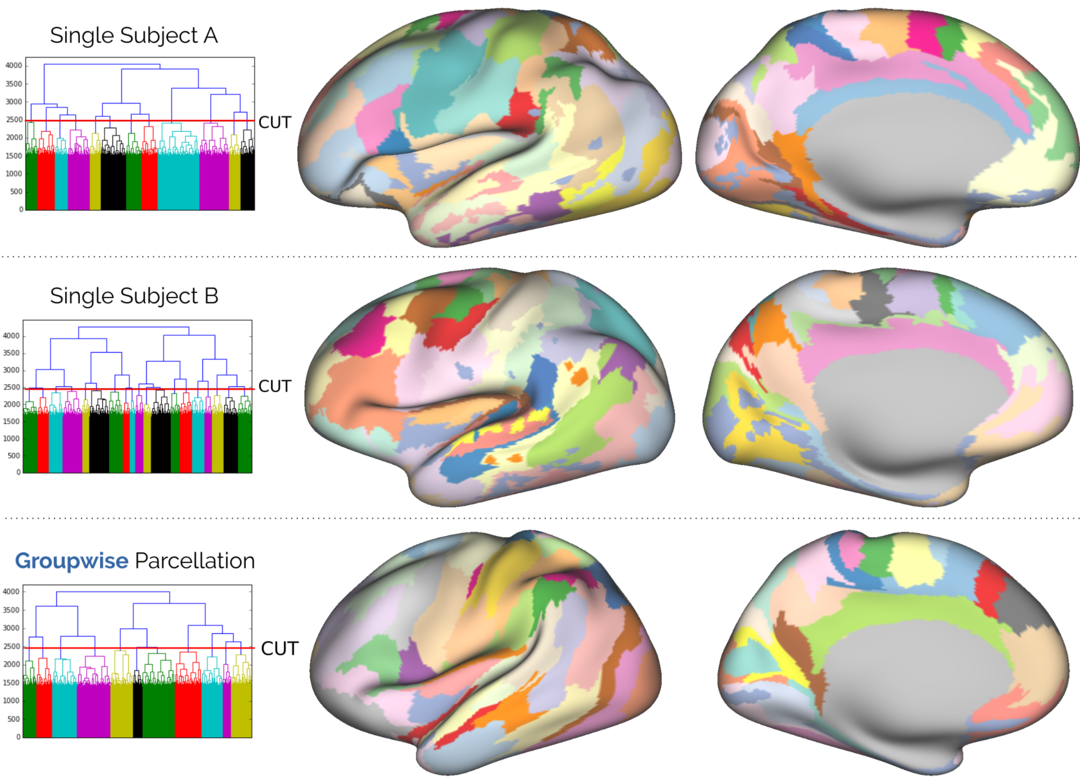
\includegraphics[width=\textwidth]{5.structural_clustering/img/single_and_group.png}
    \caption{Examples of two single-subject parcellations and the groupwise parcellations
    		 computed with our technique. All the parcellations shown have 55 parcels.
             The corresponding dendrogram for each case, along with the chosen cut height
             (red line) are shown. The groupwise parcellation
             is based on 138 subjects from the Human Connectome Project.}
    \label{fig:single_and_group}
\end{figure*}
%
\subsection{Groupwise Parcellation Technique Consistency}
To study the consistency of our technique, we randomly divided our HCP subject
sample 
in 3 disjoint groups, trying to maintain the same proportion of males and females
on each. The resulting groups had: 24 females, 22 males (group A); 23 females, 
23 males (group B) and 28 females, 18 males (group C). For each group we computed
their groupwise parcellation. The resulting parcellations at two different levels 
of granularity are shown in fig. \ref{fig:groups}.
%
\begin{figure*}
    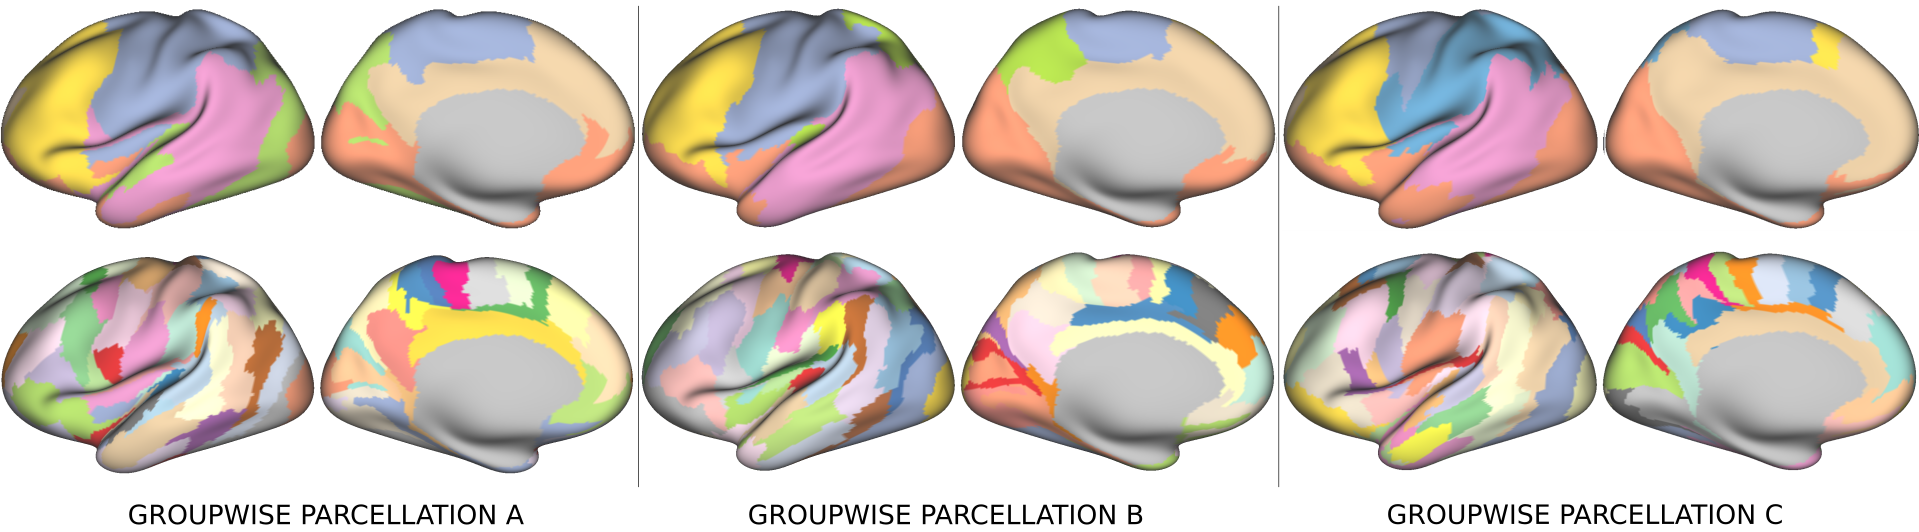
\includegraphics[width=\textwidth]{5.structural_clustering/img/groupwise_parcellations.png}
    \caption{Groupwise parcellations of 3 disjoint groups of 46 people each.
             We show results from the same dendrogram cut to get 6 parcels (upper)
             and 55 parcels (lower). Labels with best overlap in upper figures share
             the same color. Notice that there are two different shades of blue for 
             the group C.}
    \label{fig:groups}
\end{figure*}
%
To study the similarity between the obtained groupwise parcellations, we compared
them at different levels of granularity using the adjusted Rand
index~\citep{Hubert1985}. To have a baseline for the comparisons, we generated
random parcellations of the cortex and computed the similarity between them. 
We computed two types of random parcellations: The first one is an homogeneous
random parcellation with $n$ parcels, inspired in a method used by \citet{Paristot2015}. 
To compute it, we start by choosing $n$ starting points in the cortex, then, we
randomly expand each parcel
on the cortex. By comparing these random parcellations between them we compute 
the minimum obtainable Rand index by mere chance at each level of granularity. 
In the second type of random parcellation, 
we simulate the behavior of our technique. For this, we create a parcellation 
with $300$ parcels and then, we iteratively merge two parcels chosen at random until
all the parcels are merged in one. By comparing these random parcellations between
them we
obtain the minimum obtainable Rand index by a random Hierarchical Clustering
Algorithm. 
Examples of these random parcellations can be seen in Fig \ref{fig:fake_parcels}. 
The baselines presented in fig. \ref{fig:real_vs_fake} (yellow and violet lines)
were computed by comparing $1000$ of these random parcels at different levels
of granularity.
%
\begin{figure*}
    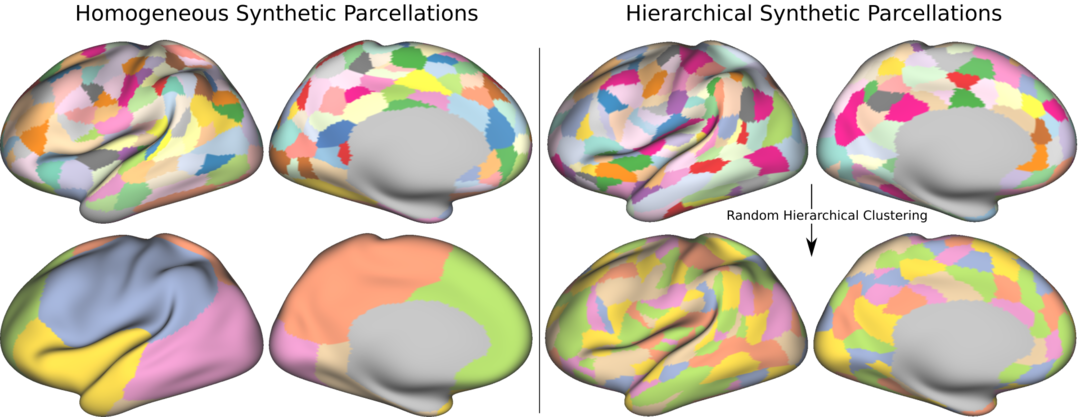
\includegraphics[width=\textwidth]{5.structural_clustering/img/fake_parcels.png}
    \caption{Examples of synthetic parcellations created to compute a baseline
             adjusted rand index. Parcellations on the left were created by 
             dividing the brain in a homogeneous way, inspired by the random
             parcellation presented in \citet{Paristot2015}. Parcellations on
             the right were created by randomly merging parcels of a coarse
             parcellation.}
    \label{fig:fake_parcels}
\end{figure*}
%
The result of comparing the groupwise parcellations of each group appear in
fig. \ref{fig:real_vs_fake}. The figure shows that the similarity between
our groupwise parcellations (lines red, green and blue) are significantly
higher than the baselines (violet and yellow). That is, the similarity
between our parcellations differs (for most cases) more than 3 standard 
deviations from the baselines' mean. Moreover, the similarity between our
results differs more
than 4 standard deviations from the comparison between synthetic hierarchical
parcels. This results show that our groupwise parceling technique creates
consistent parcellations.
%
\begin{figure*}
    \centering
    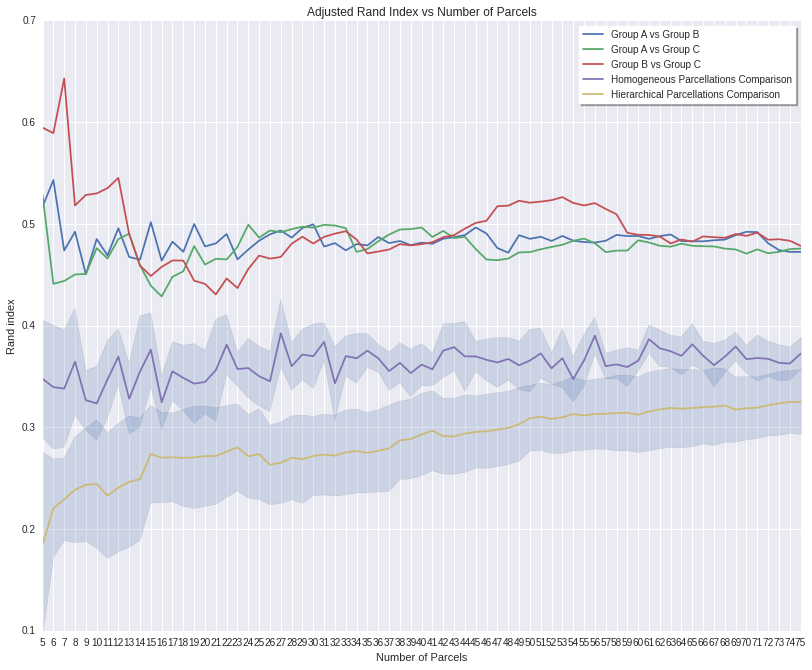
\includegraphics[width=\textwidth]{5.structural_clustering/img/real_vs_fake_parcellations.png}
    \caption{Adjusted Rand Index obtained when comparing: (red) Group A vs Group B;
             (blue) Group A vs Group C; (green) Group B vs Group C; (purple)
             Synthetic Homogeneous Parcels and (yellow) Synthetic hierarchical
             Parcels.}
    \label{fig:real_vs_fake}
\end{figure*}
%
\subsection{Relationship with a Frontal Lobe Parcellation}
Here we assess the agreement of our technique with an state-of-the-art extrinsic 
connectivity parceling technique. We do so by using our technique to parcellate 
the frontal lobe and compare our result against that of \citet{ThiebautdeSchotten2016}. 
In their work, \citet{ThiebautdeSchotten2016} use a principal component analysis (PCA)
statistical framework to parcellate the frontal lobe. They obtain a parcellation
with 12 parcels. Then, they show that each one of these parcels possess a functional
specialization by using the Decode tool\footnote{http://www.neurosynth.org/decode/}
from Neurosynth \citep{Yarkoni2011}. 
Thiebaut's parcellation is currently available in Neurovault \citep{Gorgolewski2016}
as an annotated volume\footnote{http://neurovault.org/collections/1597/}, registered
on the Colin27 template \citep{Holmes1996}. We downloaded this
parcellation and projected its parcels into a dense mesh representing the
cortex of the Colin27 template. The dense mesh had the same amount of vertices
as our chosen HCP subjects, and such vertices were coregistered with the
HCP subjects' cortical surfaces ones.

\begin{table*}[t]
\centering
\scalebox{0.9}{
  \begin{tabular}{@{}cccc@{}}
      \multicolumn{4}{c}{\textbf{Table 1. Correlation value reported (Neurosynth)}}  \\ \midrule
\textbf{Parcel} & \textbf{Term} & \textbf{$r$ (Thiebaut et al.)} & \textbf{$r$ (Ours)}\\
\textbf{1} & foot  & 0.267 & \textbf{0.319} \\
\textbf{2} & motor & 0.129 & \textbf{0.208} \\
\textbf{3} & eye field & 0.081& 0.048\\
\textbf{4} & speech production &0.077&\textbf{0.138}\\
\textbf{5} & pre sma &0.245&0.234\\
\textbf{6} & phonological &0.206&0.019\\
\textbf{7} & - &-&-\\
\textbf{8} & executive control & 0.049 & 0.042\\
\textbf{9} & - &-&-\\
\textbf{10}& semantic &0.178&\textbf{0.226}\\
\textbf{11}& social &0.137&0.110\\
\textbf{12}& semantic &0.139&0.086\\      \bottomrule
\end{tabular}}
% 
\vspace{0.3cm}
\caption*{Table 1. Spatial correlation value reported by Neurosynth for specific
                   terms in each parcel of \citet{ThiebautdeSchotten2016} and
                   for our parcels. Enumeration comes from figure~\ref{fig:frontal}.} 
\end{table*}

From the Desikan Atlas \citep{Desikan2006} of each of our HCP subjects, we
derived a groupwise mask for the frontal lobe. Then, we computed a groupwise 
parcellation with our technique, using only the tractograms in the mask. Figure
\ref{fig:frontal} shows both the parcellation downloaded from Neurovault
and our groupwise parcellation projected in the Colin template cortical surface.
The figure shows our parcellation with 10 parcels since this level of
granularity showed the best Rand index against the Thiebaut's parcellation.
The colors of each parcel in our groupwise parcellation were picked in base to
the position and amount of overlapping with the Thiebaut's parcels on the
surface. While the similarity according to the Rand index is not significantly
high ($0.4$), some visual similarity can be observed on the obtained parcellation,
particularly in the blue, yellow, orange and green parcels. Moreover, as shown in
table 1, our parcels show the same or even a higher level of functional
specialization when processed with Neurosynth.

\begin{figure*}
    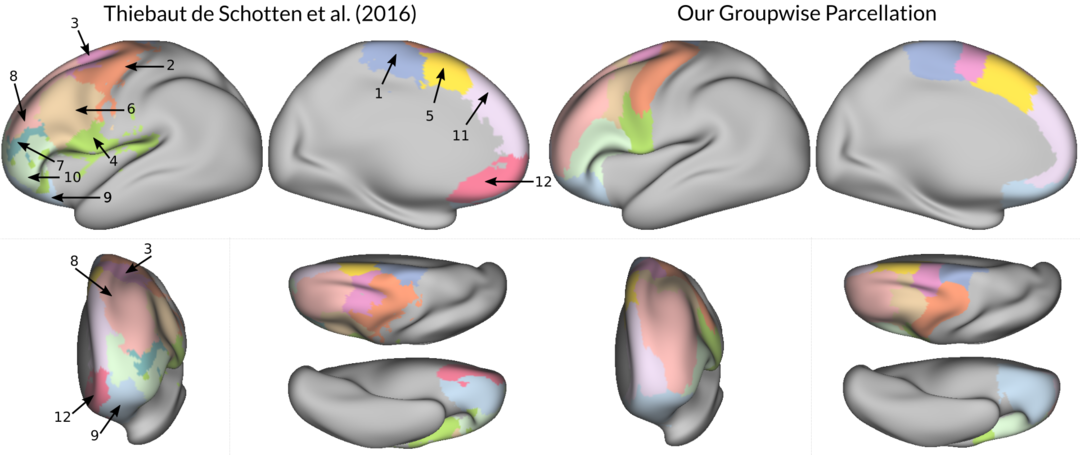
\includegraphics[width=\textwidth]{5.structural_clustering/img/frontal_lobe.png}
    \caption{\citet{ThiebautdeSchotten2016} parcellation (left) and our groupwise
    	     parcellation using only tractograms from the frontal lobe (right).
             Our parcels are colored after the parcel from \citet{ThiebautdeSchotten2016}
             with which they best overlap.}
    \label{fig:frontal}
\end{figure*}

To study the consistency of our result we computed the frontal lobe groupwise
parcellation in each of the 3 disjoint groups from the previous experiment. Figure~
\ref{fig:indices_by_lobe} shows the three obtained parcellation alongside
the Thiebaut's one. The obtained parcels show consistency, obtaining
an adjusted Rand index score of $0.61 \rpm 0.05$ between them. Finally, we
studied if the masking affected the clustering of the frontal lobe. To do so,
we applied the frontal lobe mask over a groupwise whole-brain parcellation of
the 138 subjects. The resulting frontal lobe parcellation contained 12 parcels.
This parcellation showed consistency with the one obtained by clustering only
the tractograms in the frontal lobe. More specifically, the adjusted Rand index
score between them was $0.65$. We repeated this procedure for the 3 disjoints
groups from the previous experiment. In each group, both frontal lobe parcellations
showed to be consistent, achieving an adjusted Rand index of $0.57 \rpm 0.04$.
%
\begin{figure*}
    \centering
    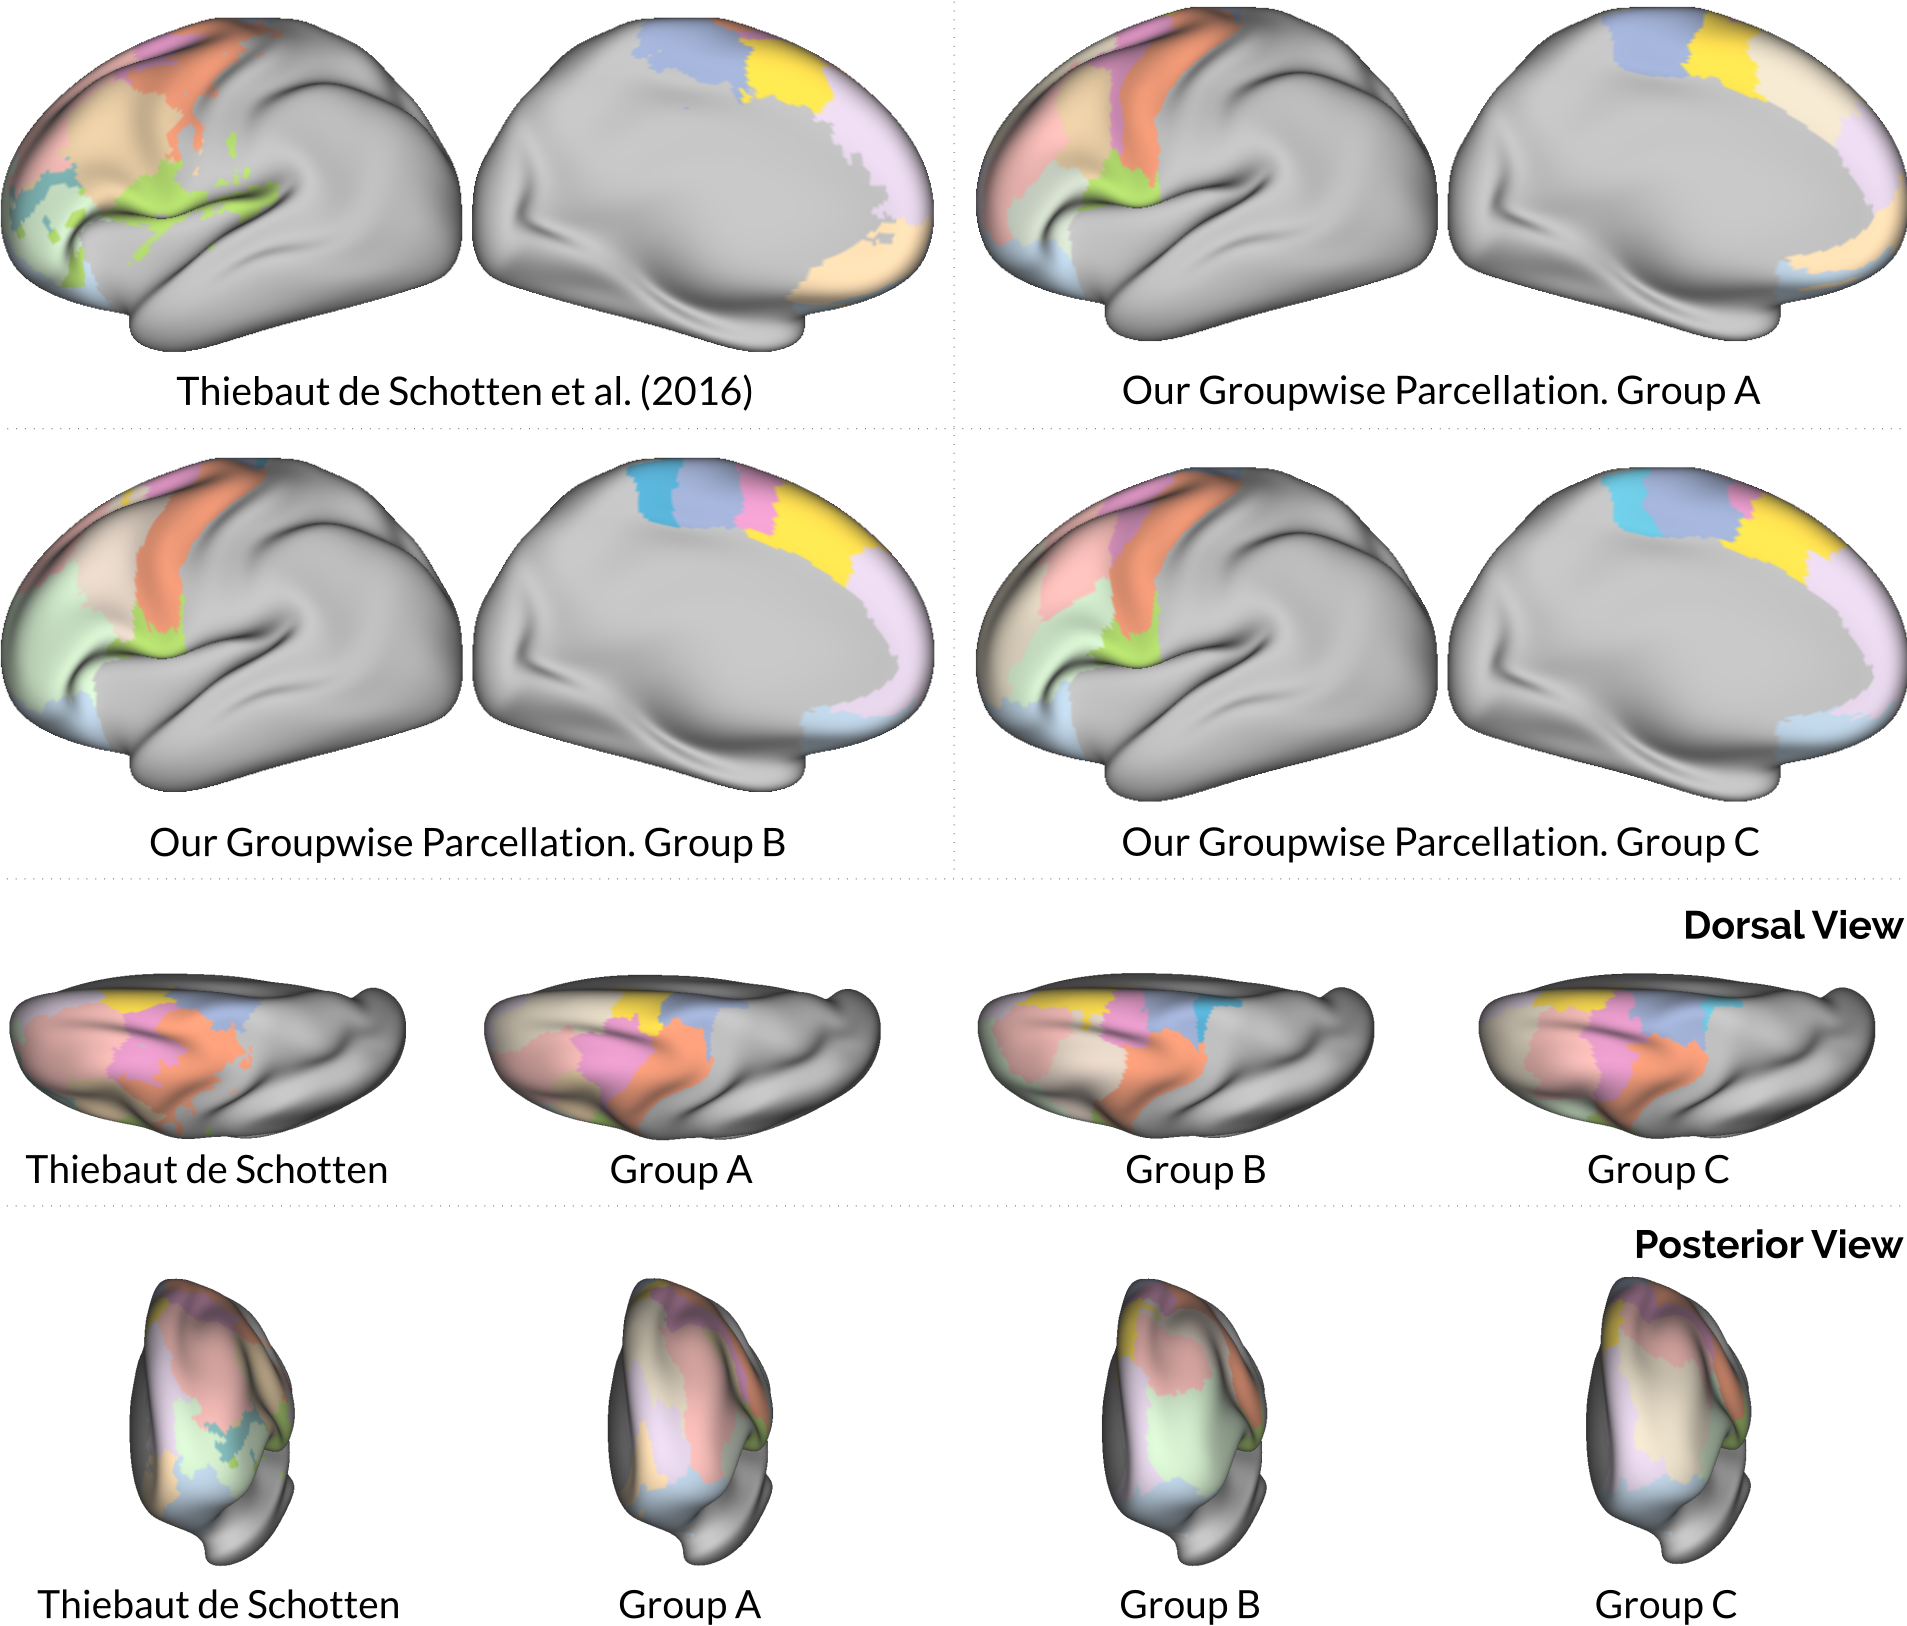
\includegraphics[width=\textwidth]{5.structural_clustering/img/3groups_frontal.png}
    \caption{\citet{ThiebautdeSchotten2016} parcellation (top-left) and our
    		 frontal lobe groupwise parcellations computed over 3 disjoint 
             groups of subjects. Our parcels are colored after the parcel from
             \citet{ThiebautdeSchotten2016} with which they best overlap.}
    \label{fig:indices_by_lobe}
\end{figure*}
%
\subsection{Anatomical Relationship and Functional Specialization of Our Parcels}
%
Here we present a proof of concept that our technique creates parcels within
anatomical boundaries and with functional meaning. To do so, first, we extracted
a parcellation with 55 parcels from the groupwise parcellation
computed from the 138 subjects. This was made to get a  parcellation with coarse
granularity while having at least the amount of 
parcels in the anatomical atlas of Desikan~\citep{Desikan2006} (36 parcels). We
compare this extracted parcellation against the Desikan Atlas and a functional
study made to every subject in the HCP~\citep{Glasser2013}.
%
\subsubsection{Relationship with Anatomical Boundaries}
%
\begin{figure*}
    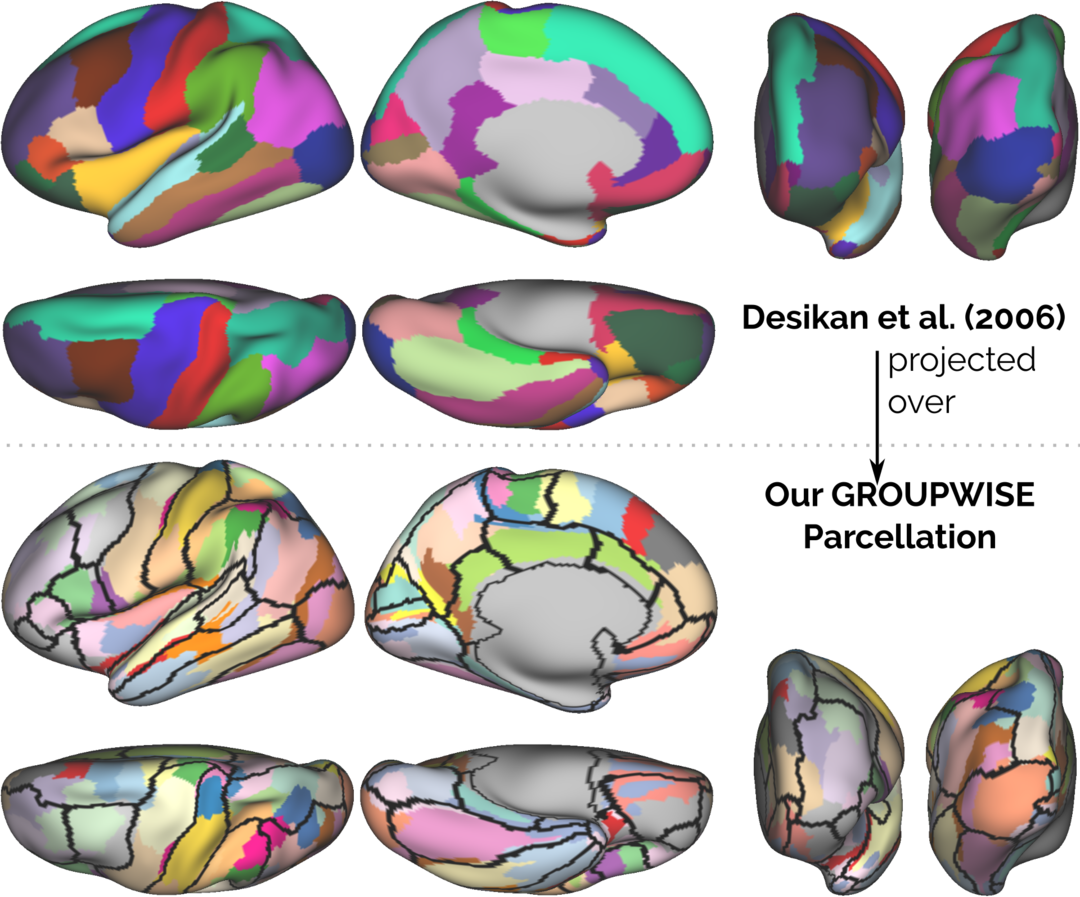
\includegraphics[width=\textwidth]{5.structural_clustering/img/anato.png}
    \caption{Relation between our pure extrinsic parcellation and the anatomical
             atlas of Desikan~\citep{Desikan2006}. Desikan atlas
             projected over the groupwise parcellation with 55 parcels.
             Insula; Cingulate; Lateral-Occipital; Fusiform; Superior Frontal;
             Lingual; Sensory and  Motor Cortex appear to be found.}
    \label{fig:anatomical_zoom}
\end{figure*}
%
To assess if some anatomical structures were present in the dendrogram and 
if our resulting parcels were subdividing them, we compared our extracted
parcellation with the Desikan atlas~\citep{Desikan2006}. To do so, we projected 
the Desikan regions over our parcels and then calculated: how many of our parcels
were contained by a anatomical region in more than a $90\%$, and which anatomical
regions were contained inside of one of our parcels. Using this criterion, the Insula; 
Cingulate; Lateral-Occipital; Fusiform; Superior Frontal; Lingual; Sensory and
Motor Cortex appear to be found as shown in Fig. \ref{fig:anatomical_zoom}.
%
\subsubsection{Functional Specialization.}
%
To study the relationship between our parcels and brain function, we projected our 
parcels over z-score maps representing responses to functional 
stimuli~\citep{Barch2013}. These maps are available as part of the HCP data, 
and represent the average activation of 100 subjects. In particular, we used
the maps related to 
the following tasks: right hand, foot and tongue movement; face, shape
recognition  and story categorization. For information on the functional tasks,
acquisition and processing of this data please refer to \citet{Barch2013}. 
Figure \ref{fig:function_motor} shows our parcels projected over contrasts
in motor tasks. In particular, our parcels are projected over the following
contrasts: tongue-average; hand movement-average and foot movement-average. 
Figure \ref{fig:function_cognition} shows our parcels projected over contrasts
in cognitive tasks: face-shape recognition; shape-face recognition and short-story
categorization. The figures show a good overlap between our parcels and the
regions with maximum activation of each task. In both figures the distribution
of z-scores inside of specific regions are shown as histograms. Further 
information about the z-score is present in tables 2 and 3. These tables show
that our parcels contain zero or few negatives values; that the mean of their
contained z-score is always positive and also, that many of those parcels 
enclose the maximum achievable z-score.

\begin{figure*}
    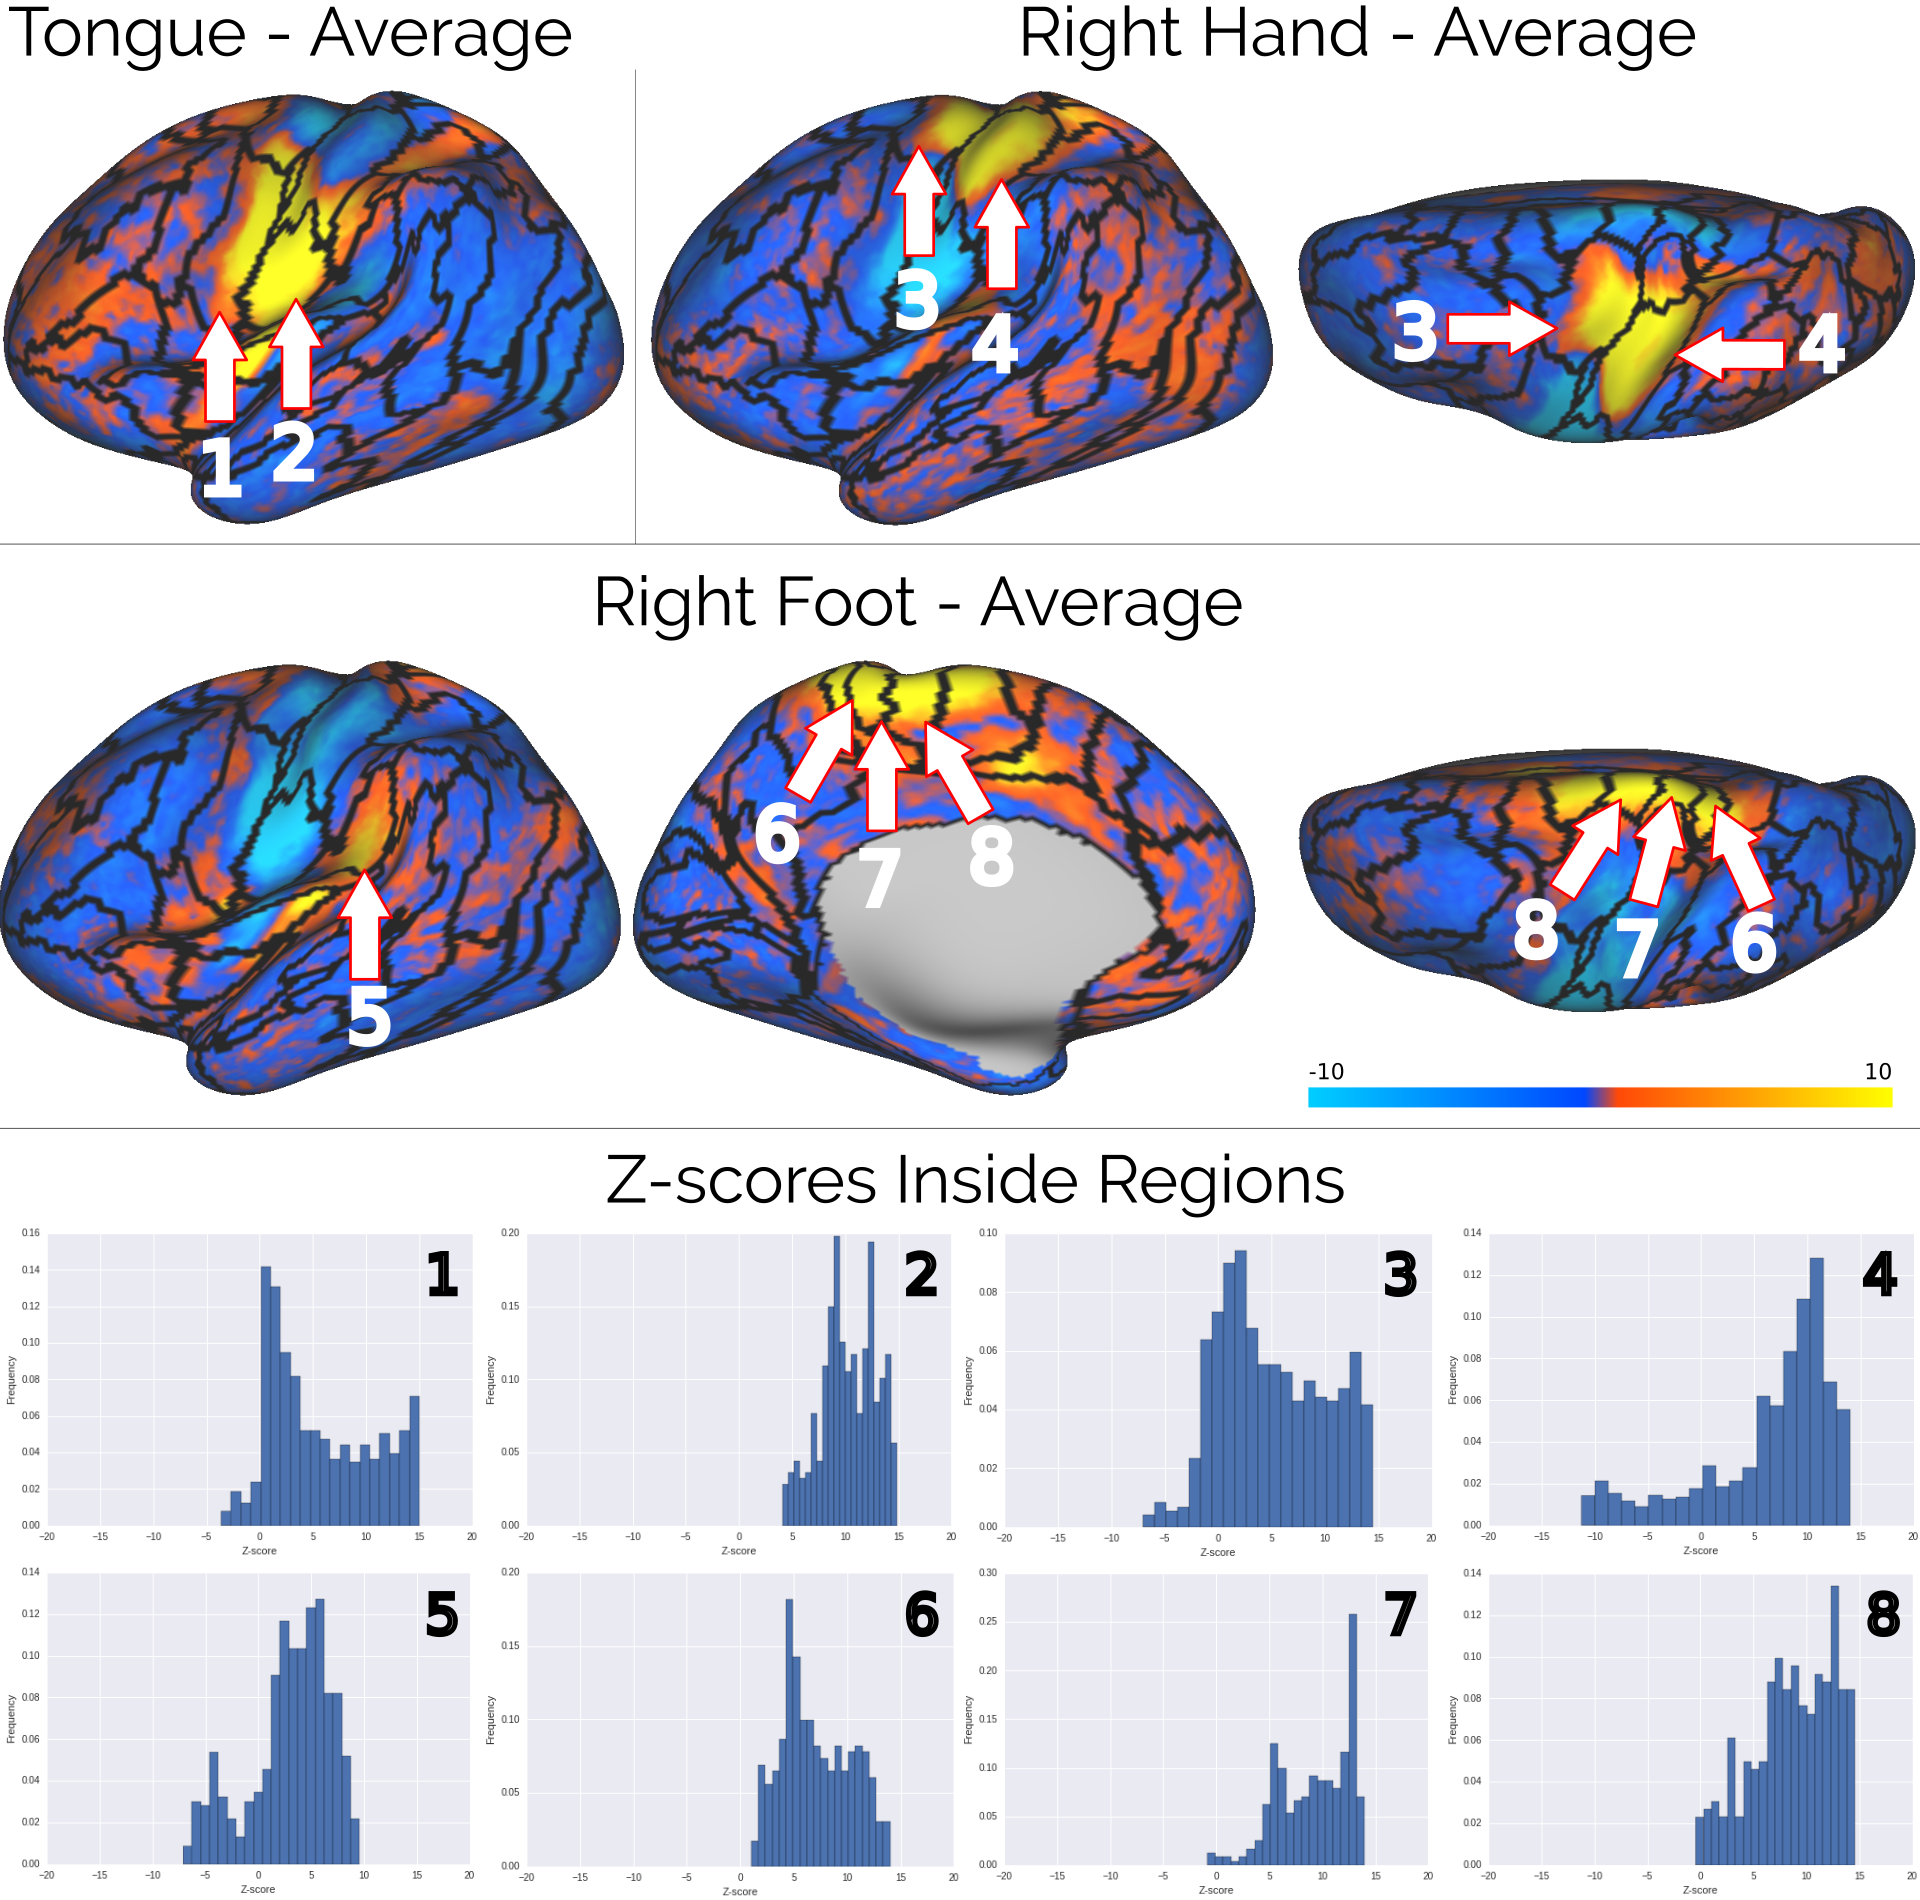
\includegraphics[width=\textwidth]{5.structural_clustering/img/function1.png}
    \caption{Our groupwise parcellation with 55 parcels projected over
             z-scores representing responses to motor tasks. Each histogram
             shows the distribution of z-score inside our parcels. The null or
             small fraction of negative values shows the functional specialization
             of our parcels}
    \label{fig:function_motor}
\end{figure*}

\begin{figure*}
    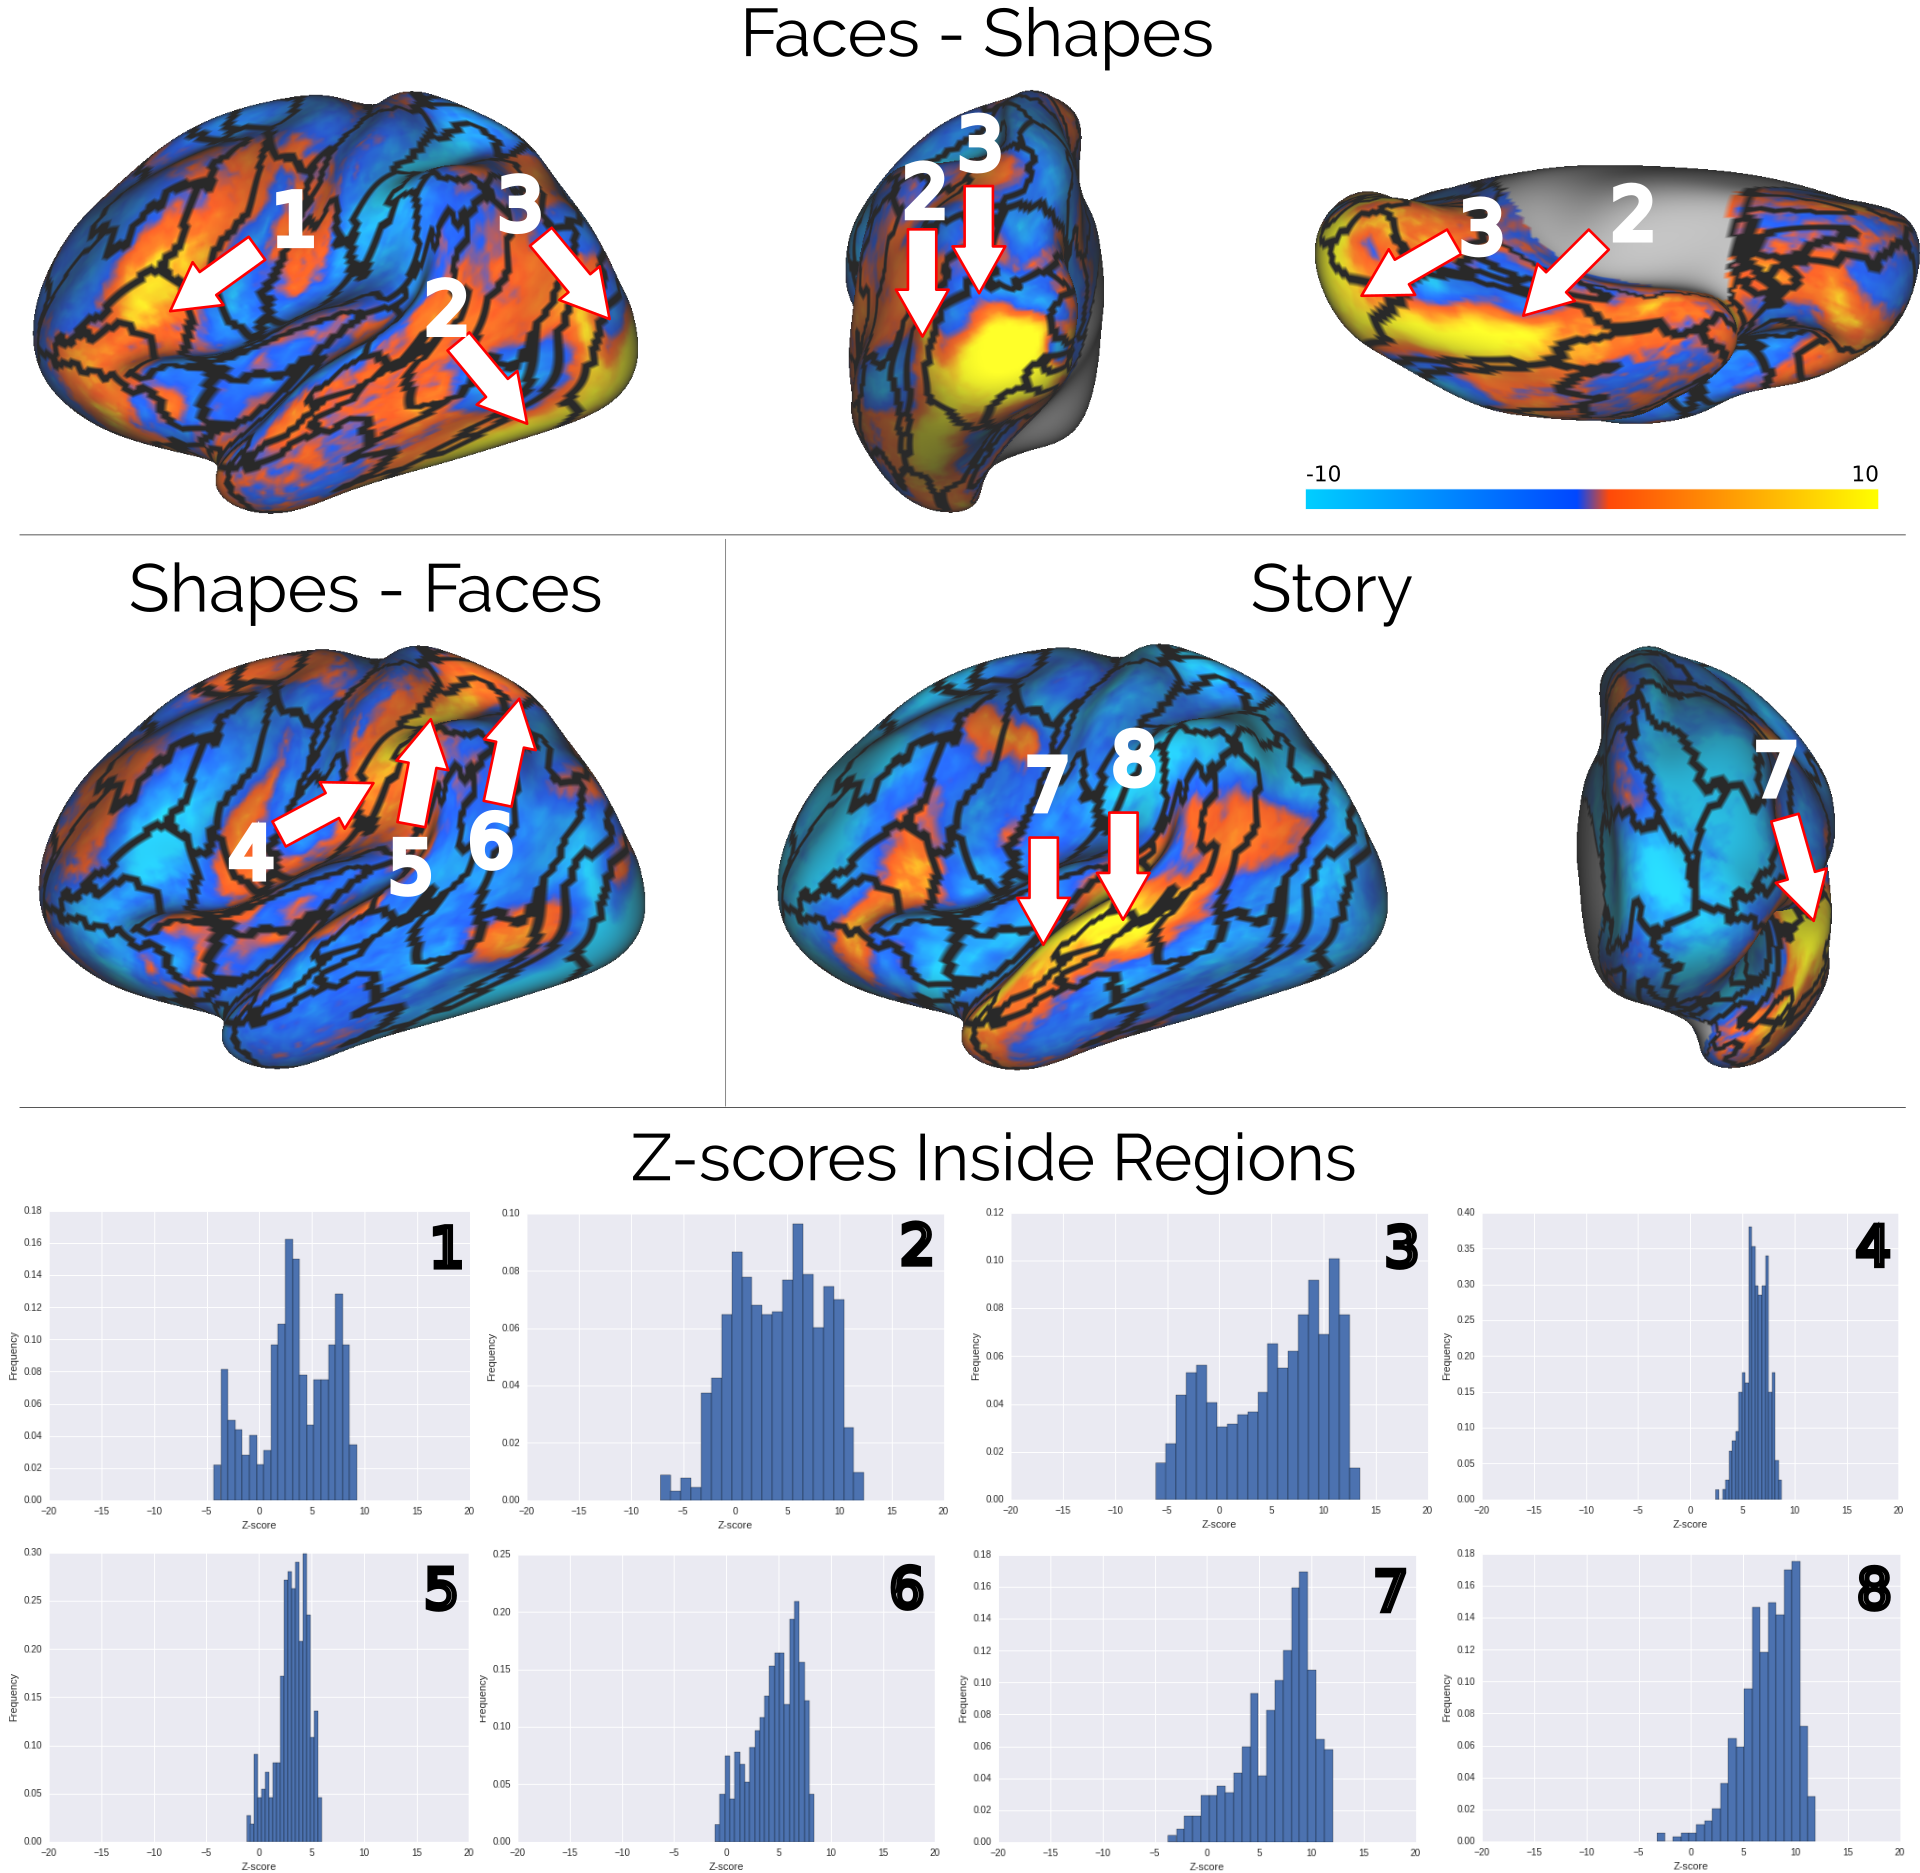
\includegraphics[width=\textwidth]{5.structural_clustering/img/function2.png}
    \caption{{Our groupwise parcellation with 55 parcels projected over
             z-scores representing responses to cognitive tasks. Each histogram
             shows the distribution of z-score inside our parcels. The null or
             small fraction of negative values shows the functional specialization
             of our parcels}
}
    \label{fig:function_cognition}
\end{figure*}

\begin{table*}[t]
\centering
\scalebox{0.9}{
  \begin{tabular}{@{}cccccc@{}}
      \multicolumn{6}{c}{\textbf{Table 2. Statistics on z-score distribution
                                 in parcels from figure
                                 \ref{fig:function_motor}}}  \\ \midrule
\textbf{Contrast} & \textbf{Parcel} & \textbf{Min.} & \textbf{Max.} & \textbf{Mean $\rpm$ Std. Dev.} & \textbf{Max. Score in Map}\\
T-Avg & \textbf{1} & -3.62  & 15.03 & $5.67 \rpm 4.91$ & 15.03 \\
T-Avg & \textbf{2} & 4.11 & 14.88 & 10.30 $\rpm$ 2.56 & 15.03 \\
RH-Avg & \textbf{3} & -7.02  & 14.50 & 5.05  $\rpm$ 4.95 & 14.50 \\
RH-Avg & \textbf{4} & -11.25  & 14.07  & 6.35 $\rpm$ 6.25 & 14.50\\
RF-Avg & \textbf{5} & -7.10 & 9.57& 2.99 $\rpm$ 3.84 & 14.56 \\
RF-Avg & \textbf{6} & 1.04& 14.01 & 7.13 $\rpm$ 3.20 & 14.56 \\
RF-Avg & \textbf{7} &-0.83 & 13.98& 9.23 $\rpm$ 3.32 & 14.56\\
RF-Avg & \textbf{8} &-0.46 & 14.56& 8.73 $\rpm$ 3.81 & 14.56 \\ \bottomrule
    \end{tabular}}
% 
\vspace{0.3cm}
\caption*{Table 2. Minimum; maximum and mean z-score contained by each of the
          parcels enumerated in figure \ref{fig:function_motor}. The highest 
          z-score of each map is reported to facilitate comparison. T-Avg: Tongue
          movement versus average; RH-Avg: Right Hand Movement versus average; RF-Avg: 
          Right Foot Movement versus average.}
\end{table*}

\begin{table*}[t]
\centering
\scalebox{0.9}{
  \begin{tabular}{@{}cccccc@{}}
      \multicolumn{6}{c}{\textbf{Table 3. Statistics on z-score distribution
      in parcels from figure \ref{fig:function_cognition}}} \\ \midrule
\textbf{Contrast} & \textbf{Parcel} & \textbf{Min.} & \textbf{Max.} & \textbf{Mean $\rpm$ Std. Dev.} & \textbf{Max. Score in map}\\
Faces-Shapes & \textbf{1} & -4.33 &  9.28 & 3.35 $\rpm$ 3.51 & 13.45 \\
Faces-Shapes & \textbf{2} & -7.16 & 12.36 & 4.01 $\rpm$ 4.09 & 13.45 \\
Faces-Shapes & \textbf{3} & -6.07 & 13.45 & 5.16 $\rpm$ 5.25 & 13.45 \\
Shapes-Faces & \textbf{4} & -5.73 &  5.37 & 0.93 $\rpm$ 1.78 &  8.79 \\
Shapes-Faces & \textbf{5} & -4.11 &  7.67 & 1.11 $\rpm$ 2.11 &  8.79\\
Shapes-Faces & \textbf{6} & -1.13 &  5.94 & 3.17 $\rpm$ 1.49 &  8.79 \\
Story & \textbf{7} & -3.72 & 12.02 & 6.72 $\rpm$ 3.35 & 12.02\\
Story & \textbf{8} & -3.24 & 11.92 & 7.41 $\rpm$ 2.50 & 12.02\\ \bottomrule
\end{tabular}}
% 
\vspace{0.3cm}
\caption*{Table 3. Minimum; maximum and mean z-score contained by each of the 
          parcels enumerated in figure \ref{fig:function_cognition}. The
          highest z-score of each map is reported to facilitate comparison. Faces-Shapes: 
          Face recognition versus shape recognition contrast; Shapes-Faces: Shape recognition
          versus face recognition; Story: Short story categorization.}
\end{table*}
%
\subsection{Relationship with a Multi-Modal Parcellation of the Cortex}
Finally, we study the (dis)similarities between our groupwise parcellation and that
of \citet{Glasser2016}. In their work, \citet{Glasser2016} compute a parcellation
of the whole cortex using information from different MRI modalities. In particular,
they use information from task functional MRI; resting state functional MRI;
myelin maps computed from T1 and T2 images and cortical thickness. It is important
to remark that dMRI data, in which our work is solely based, was not used to construct 
their parcellation.

\begin{figure*}
    \centering
    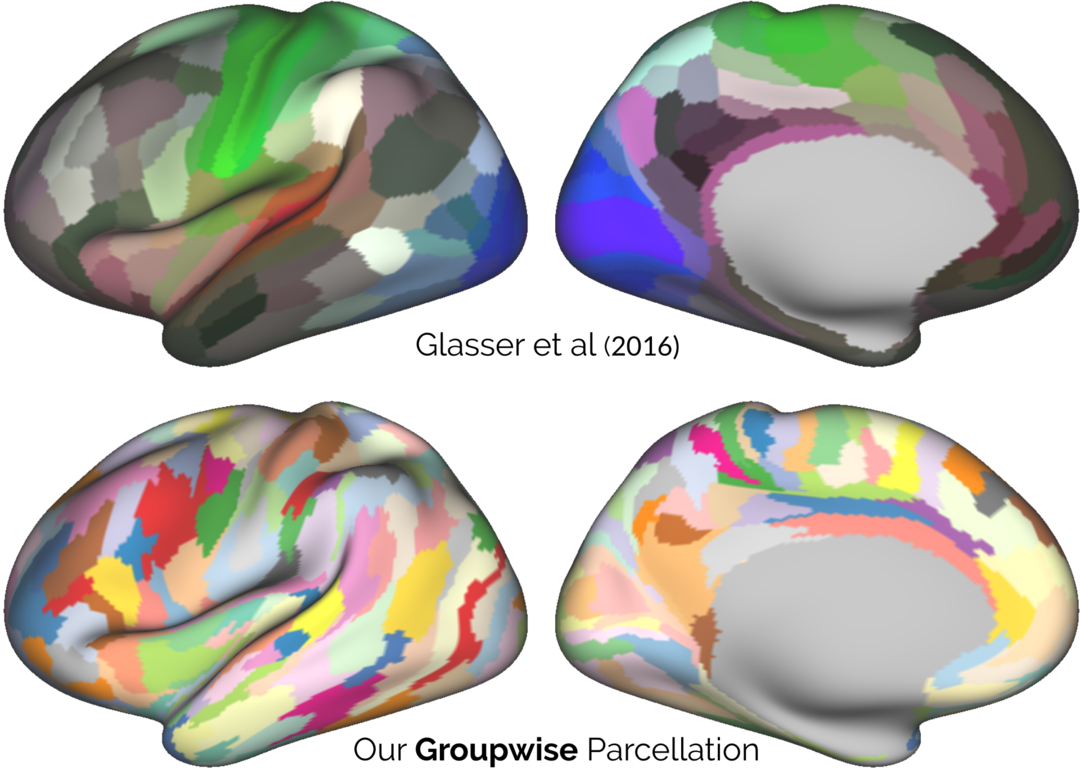
\includegraphics[width=\textwidth]{5.structural_clustering/img/glasser_and_me.png}
    \caption{\citet{Glasser2016} parcellation (upper) and our
    		 groupwise parcellations computed from 138 HCP subjects. Both 
             parcellations contain 180 parcels. There's almost no overlap according
             to the adjusted Rand index between them (0.28).}
    \label{fig:glasser_and_me}
\end{figure*}

To compare our results against Glasser's atlas, we first extracted a parcellation 
of 180 parcels from the groupwise dendrogram of our 138 HCP subjects. That is, we 
extracted a parcellation with the same number of parcels as Glasser's one. Figure
\ref{fig:glasser_and_me} show both parcellations side by side. 
We compared both parcellations using the adjusted Rand Index, obtaining a score
of 0.28. Such low score indicates that there's almost no similarity between our
result and that of \citet{Glasser2016}. Also, there's no relationship with
our groupwise parcellation with 55 parcels used in the previous section since
Glasser's parcels (finest) do not subdivide ours (coarsest).
Since Glasser's parcellation comes from functional information in the HCP, we
studied the functional specialization of its parcels in the same manner as 
previous section. Figure \ref{fig:glasser_functional} shows the histogram of
z-score contained for some parcels when using the same maps as in section
Functional Activations. It's important to remark that the z-score maps used
come from responses to functional stimuli of HCP subjects \citep{Glasser2013}.
In particular, histograms a; b and c in fig. \ref{fig:glasser_functional} show
that their subdivisions of the sensori-motor cortex contain a wide range of 
z-scores, centered in zero.

\begin{figure*}
    \centering
    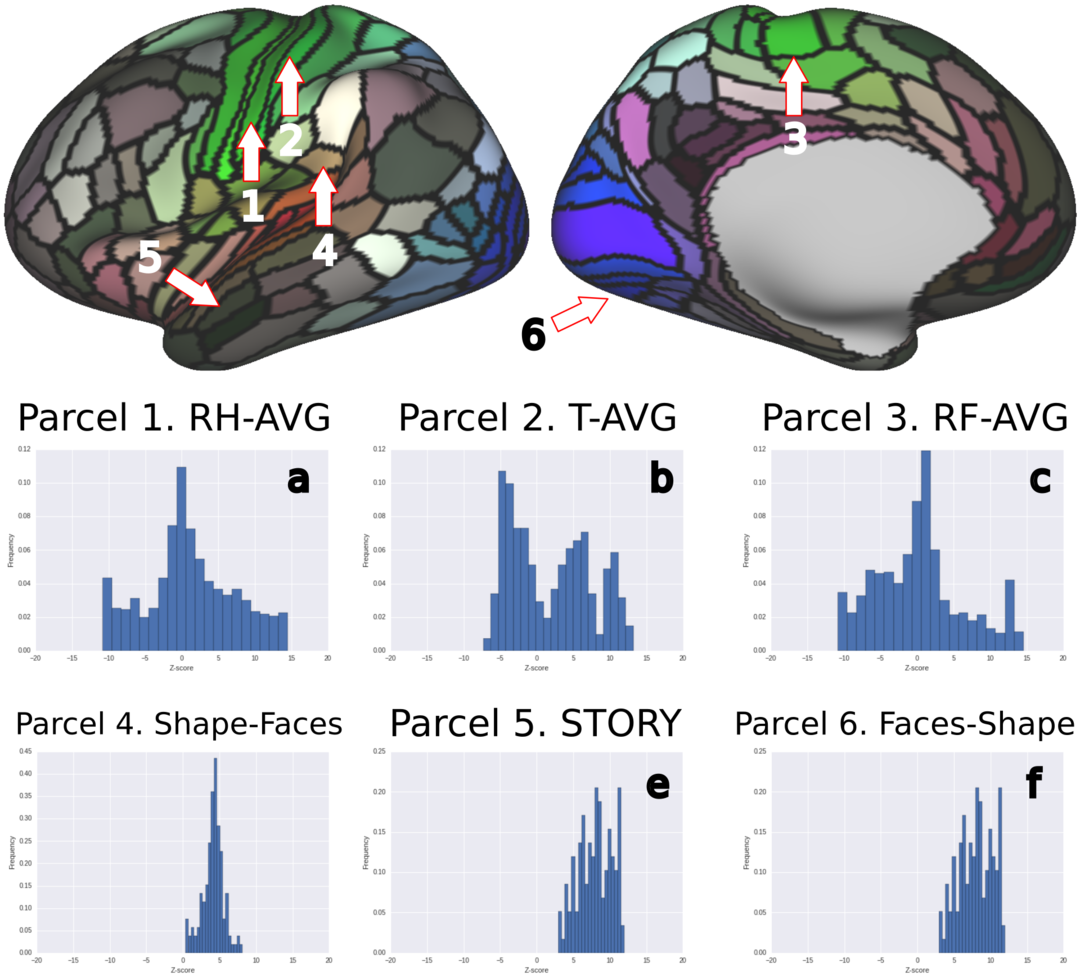
\includegraphics[width=\textwidth]{5.structural_clustering/img/glasser_functional.png}
    \caption{\citet{Glasser2016} parcellation (upper) and histograms of 
             z-score contained in different parcels for different functional
             task. (a) Histogram for parcel 1 for the contrast related to
             Tongue movement. (b) Histogram for parcel 2 for the contrast
             related to Tongue movement. (c) Histogram for parcel 3 for the
             contrast related to Right Foot movement. (d) Histogram for parcel
             4 for the contrast Shape recognition vs Face recognition. (e)
             Histogram for parcel 5 for the contrast related to Story
             Categorization.
             (f) Histogram for parcel 5 for the contrast Face recognition vs Shape
             recognition. The histograms (d); (e) and (f) correspond to the parcels
             with the greatest mean z-score of their respective tasks.}
    \label{fig:glasser_functional}
\end{figure*}
%
\section{Discussion}
%
In this work we presented a parsimonious statistical model for long-ranged
axonal connectivity. Our model (section \ref{sec:cortical_model}), assumes that
the cortex is divided in patches of homogeneous extrinsic connectivity, as histological
results showed in the macaque brain \citep{Schmahmann2006}. By borrowing ideas
from statistical clustered data models~\citep{Pendergast1996}, our model accounts
for the variability in the axonal connections of a patch's neurons and for 
variability in patch boundaries across subjects.

Taking advantage of our proposed model, in Section \ref{sec:parceling_methodologies}
we presented an efficient
technique to parcellate the cortex based on its extrinsic connectivity. Our
technique uses only dMRI information, without the need of relying on
initial parcellations~\citep{Clarkson2010}. Also, our technique allows 
parcellation of the whole cortex, overcoming the problem of working with only part
of it~\citep{Lefranc2016, Roca2009, ThiebautdeSchotten2014, ThiebautdeSchotten2016}.
Additionally, our technique allows creation of both single subject and
groupwise parcellations. Our groupwise parcellation technique relies on anatomical
seed-correspondence across subjects. In our experiments, this is achieved as
each HCP subject possess a coregistered dense mesh representing they cortical
surface \citep{Glasser2013}. Given the anatomical differences across-subjects,
this purely anatomical matching of seeds is probably sub-optimal. However, it
allows us to compute single and groupwise parcellations independently. By doing
this, we avoid the need to impose constraints between our single and group
parcellations~\citep{Clarkson2010, Roca2010, Paristot2015}.

Inspired by \citet{Moreno-Dominguez2014}, our technique uses Hierarchical
Clustering to comprise multiple granularities of the same parcellation in a
dendrogram. This allows us to overcome the need of other techniques~\citep{Paristot2015}
to specify an expected number of clusters. Hence, we don’t need to recompute the
whole pipeline each time a new parcellation is required. As in
\citet{Moreno-Dominguez2014}, we also create the dendrogram using only one
comprehensive parameter: the minimum size of each cluster. This
parameter imposes the local coherence criterion. Our fundamental difference
with Moreno-Dominguez' technique is how we compare and merge tractograms during
the clustering process. \citet{Moreno-Dominguez2014} use Centroid
Clustering~\citep{Murtagh1985} with the cosine distance. This can lead to an
erroneous parcellation since the centroid criterion doesn't minimize the cosine
distance between points. Also, their method creates dendrograms with inversions
\citep{Murtagh1985}, which are then removed heuristically. In our case, using a
Logistic Random Effect model (eq. \ref{eq:ran_eff_model}) allowed us to transform
the tractograms into a Euclidean space (sec. \ref{sec:parceling_methodologies})
and compare them using the Euclidean distance. In doing this, it is important to
remark that we are making a trade off. Since we are comparing high-dimensional
vectors with the Euclidean distance, we are probably affected by the dimensionality
curse \citep{Beyer1999}. However, working in an Euclidean space possess many
advantages. The first advantage is that we can compute clusters with minimum
intra-cluster variance by using Ward's Hierarchical method. We can use this algorithm
since its only hypothesis is that the features to cluster are in a Euclidean space.
Also, since we work with the Euclidean distance, we can apply the Lance and Williams
\citep{Lance} formula during clustering. This formula gives us the dissimilarity
between the new centroid created at each step and the rest of the existing
tractograms in constant time. As far as we know there's no Lance and Williams
formula when using the cosine distance with the centroid linkage. This allows
us to lower the time complexity of our algorithm with respect to Moreno-Dominguez.
Since we use Ward's clustering, our resulting dendrograms do not have
inversions, which means that we don't need to post-process them. Another
advantage is that we can retrieve a parcellation from the dendrogram using a
simple technique: horizontal cut~\citep{Murtagh2011}. While other methods to cut
the dendrogram exist~\citep{Murtagh2011}, horizontal cut is sufficient to solve
our Gaussian Mixture Model (eq. \ref{eq:ran_eff_model}) as shown in
\citet{Gallardo2017}. Finally, even if our algorithm is probably affected by
the dimensionality curse, our parcellations showed to be consistent
across-groups and in agreement with extant parcellations in the literature.
%
\subsection{Our Groupwise Parcellations are Consistent Across Similar Groups:}
%
We assessed the consistency of our groupwise parcellation by quantifying the
consistency across 3 disjoint groups of 46 subjects each. The consistency is
shown by the adjusted
Rand index in Fig.~\ref{fig:real_vs_fake}, which quantifies consistency across
parcellations~\citep{Hubert1985}. As seen in Fig.~\ref{fig:real_vs_fake} whole-cortex
parcellations obtained with our method are consistent across groups, and the
Adjusted Rand Index is significantly higher, i.e.\ more than 3 standard
deviations, for all granularities when compared with the null case of
randomly-generated parcellations. 

Our whole-cortex groupwise parcellation reaches a maximum consistency score when
the cortex is divided in 6 regions, see Fig.~\ref{fig:real_vs_fake}.  As seen in
Fig. \ref{fig:groups}, these parcellations are consistent with specific
anatomo/functional networks: the frontal lobe section anterior to the prefrontal
cortex is shown in yellow; the sensorimotor area is shown in cyan, the cingulate
area is shown in beige; the fronto-occipital connection in orange, and the
temporo-parietal system in pink. 

\subsection{Our Method Creates Parcels in Agreement With a Single-Lobe Parceling
            Technique Extant in the Literature.}
%
We showed that our technique obtains results similar to another method extant
in the literature. We did so by parceling only the frontal and showing the visual
similarity between our resulting parcels and those obtained by
\citet{ThiebautdeSchotten2016}. Moreover, the blue, pink and green parcels
in fig. \ref{fig:frontal} share not only similar boundaries and location, but
also functional specialization (Table 1). In some cases our parcels possess even higher
spatial-correlation with functional task according to
Neurosynth's \citep{Yarkoni2011} Decode tool\footnote{http://neurosynth.org/decode/}. We assessed the 
consistency of our obtained groupwise parcellation by computing the groupwise 
frontal lobe parcellation of three disjoints groups of 46 subjects and comparing
them using the adjusted Rand index. The obtained value of $0.61$ shows that our
parcellation of the frontal lobe is consistent across groups.
%
\subsection{Our Method Creates Several Parcels in Agreement with Brain Anatomy.}
%
We showed that many of our parcels are in agreement with brain anatomy. 
In particular, we showed that in our groupwise parcellation, with 55 parcels,
the following anatomical structures appeared to be found: Cingulate; Insula;
Lateral-Occipital; Fusiform; Superior Frontal; Lingual; Motor and Sensory cortex.
Here we discuss why some of these parcels were found and how are their 
conectivity fingerprints.
In the case of the Cingulate, its fingerprint, shown in fig. \ref{fig:conn_fing}, is
strongly related with the Cingulate Fascicle (CF) pathway. This
is consistent with the 
fact that the seeds located in the Cingulate will end up into the CF after being 
pushed in the white-matter. In the case of the Insula, each subdivision
showed a specific pattern of connectivity as shown in fig. \ref{fig:conn_fing}. 
These parcels show a gradient of connections from the occipital lobe to the frontal
lobe consistent with that of \citet{Ghaziri2015}. In the
Lateral-Occipital region, we see a specific pattern of local connectivity which
cannot be attributed to gyral bias since the Lateral-Occipital covers many sulci
and gyrus. In the case of the fusiform, it is almost completely contained in one
of our parcellations, which goes from the Fusiform up to the Lateral-Occipital
(fig. \ref{fig:anatomical_zoom}). 
This could add evidence to the hypothesis that the Fusiform plays a role in visual
tasks \citep{Kanwisher2006, Yeatman2014}. Finally, the Motor and Sensory cortex appear to be
found. While the
appearance of each gyri is most probably because of gyral bias \citep{VanEssen2014},
the parcels inside them show specific patterns of structural connectivity (fig.
\ref{fig:conn_fing}), and, as seen in section 3.5.2, functional specialization.

\begin{figure*}
    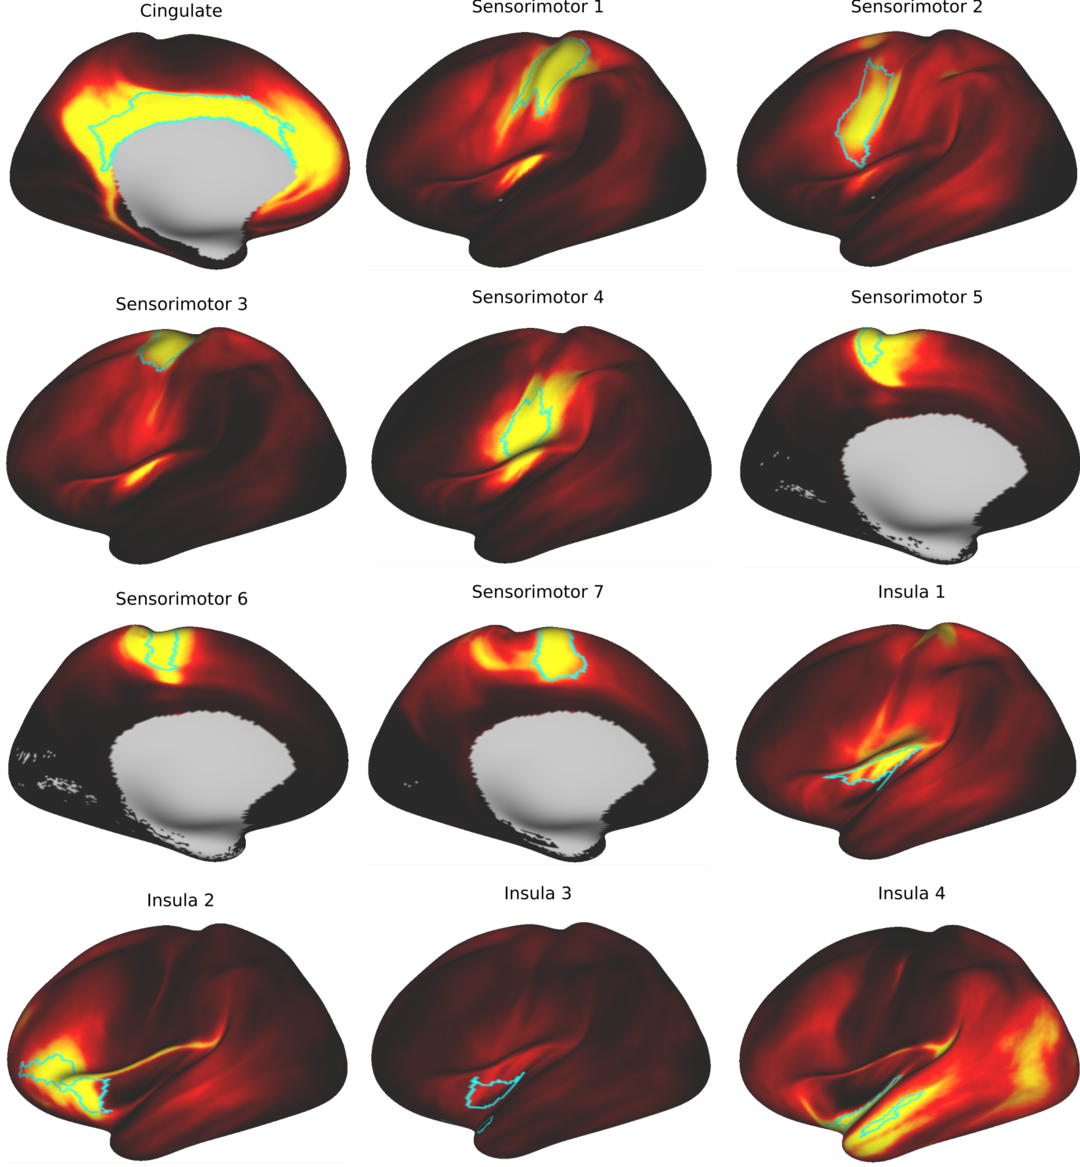
\includegraphics[width=\textwidth]{5.structural_clustering/img/conn_fing.png}
    \caption{Connectivity fingerprint for different parcels in our groupwise
             parcellation. The names in the titles are given after the anatomical
             structure that they subdivide (or contain, as with the Fusiform). }
    \label{fig:conn_fing}
\end{figure*}


\subsection{Our Results Show a Close Relationship Between Structural Connectivity
and Brain Function.}
%
We assessed the functional specialization of some of our parcels by showing
how they overlap with responses to functional and cognitive tasks measured
with fMRI. In particular, for all the studied tasks, the parcels contained
a higher proportion of positive values than negative ones as expressed by the
positive mean values reported in tables 2 and 3. For some parcels there
were not even negative values. Moreover, several of the histograms on figures
\ref{fig:function_motor} and \ref{fig:function_cognition} show a high frequency
of z-score values greater than 5, which indicate a significant correlation with
functional activation. Therefore, our results show, for some tasks, the
strong relationship between extrinsic connectivity and functional
specialization in the human brain cortex. 
%
\subsection{Our Parcels Are Not Similar to Those Obtained by Glasser et al. (2016) But 
			Possess Better Functional Specialization for Motor Tasks.}
Our parcels were not related to those of \citet{Glasser2016}. This is shown by the
obtained adjusted Rand index score between them (0.28). It's important to remark that
our parcels are purely based on extrinsic connectivity, meanwhile those of \citet{Glasser2016}
do not use dMRI information. Glasser's parcels are mostly based on myelin and functional information.
In particular, their subdivision of the sensori-motor cortex (green parcels in fig.
\ref{fig:glasser_and_me}) is mostly based in Myelin maps as shown in Figure 4.a of 
\citet{Glasser2016}. Because of this, their parcels in the sensori-motor cortex contain 
a wide range of z-scores when compared with responses to functional stimuli as shown by
histograms a; b and c in fig.
\ref{fig:glasser_functional}. In contrast, our parcels in the sensori-motor cortex,
for a coarser parcellation, show a good overlap with function and are in agreement with
the motor strip mapping as discussed in the previous section. Also, for the case of story
categorization; shape recognition and face recognition, our parcels show a similar
distribution of z-scores (fig. \ref{fig:function_motor}) than those with the highest 
mean z-scores of \citet{Glasser2016} (parcels d; e and f of  fig. \ref{fig:glasser_functional}).
%
\section{Conclusion}
%
Understanding how the brain is structurally organized and how it constraints
functionality is an open question in neuroscience. Recent advances in
acquisition and modeling techniques on dMRI have facilitated to study 
axonal connectivity in the brain. However, parceling the whole cortex based
on a structural criterion remained challenging. In this chapter we presented a 
connectivity model; framed tractography within our model and 
presented a parceling technique that allows parcellation
of the whole brain in both single subject and groupwise cases.

However, a new question rises, given two single subject parcellations, how to
match the parcels across them?. Even when our results show that our technique is stable
across groups of subjects, some variability still exists, and finding a
correspondence between two parcellations is not a trivial task. The 
following chapter of this thesis will work on this problem.

%\section{References}
%\bibliographystyle{elsarticle-harv}
\chapterbib

    \chapter{Solving the Cross-Subject Parcel Matching Problem using Optimal Transport}
\label{ch:matching}

\section{Overview}
Matching structural parcels across different subjects is an open problem in
neuroscience. Even when produced by the same technique, parcellations tend to
differ in the number, shape, and spatial localization of parcels across subjects.
In this chapter, we propose a parcel matching method based on Optimal Transport.
We test its performance by matching parcels of the Desikan atlas, parcels based
on a functional criteria and structural parcels. We compare our technique against
three other ways to match parcels which are based on the Euclidean distance, the
cosine similarity, and the Kullback-Leibler divergence. Our results show that
our method achieves the highest number of correct matches.

This work was presented as part of the MICCAI 2018~\cite{Gallardo2018}.

\section{Introduction}
Brain organization displays high variability across individuals and species.
Studying brain connectivity therefore faces the challenge of locating homogeneous
regions while accounting for this variability. Different techniques have been
proposed to parcellate the brain based on its structural connectivity. However,
matching the resulting parcels across different subjects is still an open
problem in neuroscience. Even when produced by the same technique, parcellations
tend to differ in the number, shape, and spatial localization of parcels across
subjects \cite{Jbabdi2013}. Current theories hold that long-range structural 
connectivity, namely, extrinsic connectivity, is strongly related to brain
function \cite{Passingham2002}. Therefore, being able to match parcels with
similar connectivity across subjects can help to understand brain function while
also enabling the comparisons of cortical areas across different
species \cite{Mars2018}.
% Sam: In MIC, one of the interest is image segmentation/registration. Can you make a very clear link to this?

Most of the current methods to match parcels across subjects are strongly
linked to the technique used to create them. For example,
Moreno-Dominguez et al. \cite{Moreno-Dominguez2014} seek correspondences between
dendrograms created by means of Hierarchical Clustering. 
Parisot et al. \cite{Paristot2015} impose the consistence of parcels across
subjects while creating the parcellation. In recent works Mars et al. propose
to use the Manhattan distance, cosine similarity \cite{Mars2016} or the
Kullback–Leibler (KL) divergence \cite{Mars2018} to compare and match connectivity
fingerprints, successfully identifying common areas across humans and primates.

In this work, we propose to match parcels based on their extrinsic connectivity
fingerprint using Optimal Transportation theory. Optimal Transport (OT) is a
technique that seeks the optimal way to transport mass between probability
distributions. While KL divergence computes the difference between two
distributions, OT computes a matching between them. In particular, our method
adopts a discrete regularized version of Optimal Transport (OT), which has been
presented in Gayraud et al.~\cite{nathalie} and Courty et al.~\cite{remi} as a
solution to the domain adaptation problem.

\begin{figure*}[t!]
\centering
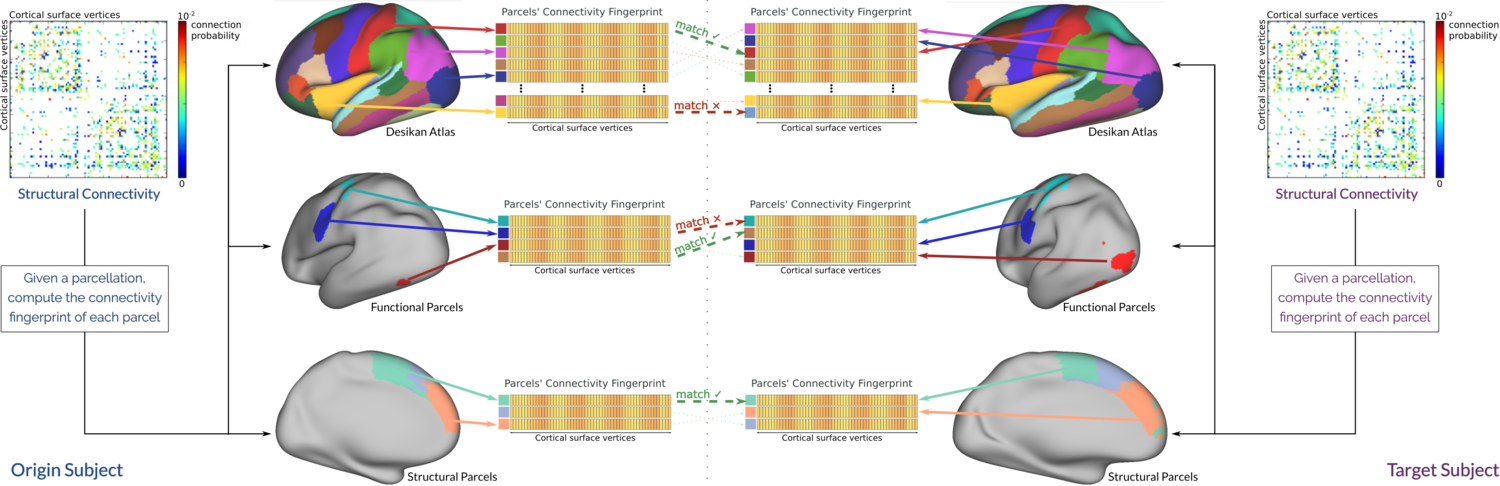
\includegraphics[width=1\textwidth]{6.matching/img/method}
\caption{From the cortico-cortical structural connectivity matrix of a subject, we can estimate the connectivity fingerprints of each parcel in three different types of parcellations. For each parcellation we compute the amount of correct matches (green lines) that each matching technique produces.}
\label{fig:method}
\end{figure*}

We validate our method with four different experiments. In the first experiment,
we test the feasibility of our method by generating parcels with synthetic
connectivity fingerprints and matching them. In the second one, we show that
our technique is able to match parcels of the same atlas across subjects. We
use the anatomical atlas of Desikan \cite{Desikan2006} as its parcels have
high spatial coherence and consistent connectivity profiles across
subjects \cite{DeReus2013}. Finally, we show the capacity of our method to
match parcels generated with the same criteria but have some spatial
cross-subject variability. We assess this for two different situations. In the
first one, we derive the parcels from functional activations~\cite{Barch2013}.
We use responses to motor and visual stimuli since they have been shown to be
strongly related to structural connectivity~\cite{Osher2016, Penfield1954}. 
In the second one, we divide the Lateral Occipital Gyrus in 3 parcels using
a structurally-based parcellation technique  \cite{Gallardo2017a}. We use
the Lateral Occipital Gyrus since it has been shown to have a consistent
parcellation across subjects \cite{ThiebautdeSchotten2016, Gallardo2017a}.
The outline of the last three experiments can be seen in Figure~\ref{fig:method}.

In each experiment, we compare our technique against three other ways to match
parcels based on the Euclidean distance; the cosine similarity; and the
Kullback-Leibler divergence. Our results on real data show that our method
based on OT always achieves the highest number of correct matches.


\section{Methods}

Given two subjects with their respective parcellations, we compute their parcel matching by considering one as the origin and the other one as target. 
More formally, let $X^a = \{x^a_i\}_{i=1}^{N_a}$, $x^a_i \in \Omega^a \subset \mathbb{R}^n$ be an origin dataset where $N_a$ denotes the number of parcels; $x^a_i$ is the extrinsic connectivity fingerprint of parcel $i$; and $n$ denotes its dimension. We wish to recover a matching between $X^a$ and a target dataset ${X^b = \{x^b_i\}_{i=1}^{N_b}}$, $x^b_i \in \Omega^b \subset \mathbb{R}^n$.
% Sam: What is an extrinsinc connectivity fingerprint? Where does it come from?
% You talk about extrinsic connectivity but you don't use the word fingerprint in the intro.
% Maybe start this section with a word on diffusion, tractography, and the inputs you need.

% Sam: How do you represent a matching? A permutation matrix? Nath: originaly yes, but it didn't fit. Is the structure that represents the matching important? Sam: well, this paragraph sounds like a problem statement, but at the end I still don't now what you are trying to find.

In this section, we start by formulating our regularized discrete OT-based method
and proceed by presenting three ways of computing this matching that are based
on the Euclidean distance; the cosine similarity; and the KL-divergence.

\subsection{Discrete Regularized Optimal Transport}

Optimal Transport (OT) theory boils down to finding the optimal way to transport
or redistribute mass from one probability distribution to another with respect
to some cost function. In this work, since the datasets $X^a$ and $X^b$ are
discrete datasets, we use their empirical probability distributions and apply
the discrete formulation of OT~\cite{nathalie,remi} to solve the parcel matching
problem. A simplified example of how our method proceeds is presented in
Figure~\ref{fig:otprob}.

Assume that $X^a$ and $X^b$ follow probability distributions $p_a(x^a)$ and
$p_b(x^b)$, respectively. We suppose that $X^a$ has undergone a transformation
$\mathbf{T}:\Omega^a \rightarrow \Omega^b$, such that
$p_b(\mathbf{T}(x^a)) = p_b(x^b)$. We wish to recover $\mathbf{T}$ and use it
to match the parcels of $X^a$ and $X^b$. Using discrete regularized OT we 
compute a transport plan $\gamma_0$ between these two probability distributions.
This transport plan is a doubly stochastic matrix which minimizes a certain
transportation cost $C$ over the vectors of $X^a$ and $X^b$. In other words,
it defines the optimal exchange of mass between the two probability distributions.
We use $\gamma_0$ to compute an estimation $\hat{\mathbf{T}}$ by selecting the
pairs of vectors, i.e., parcels that exchange the most mass. 
% Sam: I think this requires a bit more detail. What do you mean by a transport plan? I am guessing its
% related to T. Then, how does that transport plan give you a matching 
%Nath: Hopefully it is better explained now

Since $p_a(x^a)$ and $p_b(x^b)$ are not known, we use the corresponding empirical distributions $\mu_a = \sum_{i=1}^{N^a} p_i^a\delta_{x^a_i}$ and $\mu_b =\sum_{j=1}^{N^b} p_j^b\delta_{x^b_j}$ instead, where $p_i^a$ and $p_j^b$ are the probability masses associated to each sample. However, given that the dimension of our data depends on the number of vertices in the cortical mesh, the curse of dimensionality makes the estimation of $\mu_a$ and $\mu_b$ intrinsically difficult. We therefore simply assume a uniform probability distribution over all vectors, $p_i^a = \frac{1}{N^a}$ and $p_j^b = \frac{1}{N^b}$. We compute the transport plan $\gamma_0$ such that, if
% Sam: here the transport plan is gamma? How is it related to T?
% Explained in the intro and later

\begin{equation}
{\mathcal{B} = \big\{ \gamma \in (\mathbb{R}^+)^{N_a\times N_b} \mid \gamma \mathbf{1}_{N_b} = \frac{1}{N^a}\mathbf{1}_{N_a}, \gamma^{\mathbf{T}} \mathbf{1}_{N_a} = \frac{1}{N^b}\mathbf{1}_{N_b}  \big\}}
\end{equation}
denotes the set of all doubly stochastic matrices whose marginals are the probability measures $\mu_a$ and $\mu_b$, where $\mathbf{1}_N$ is an $N$-dimensional vector of ones, then $\gamma_0 \in \mathcal{B}$ is the output of the following minimization problem.
% Sam: Don't add a new line after equations or latex adds a new paragraph indentation.

\begin{figure*}[t!]
    \centering
    \begin{subfigure}[t]{0.32\textwidth}
        \centering
        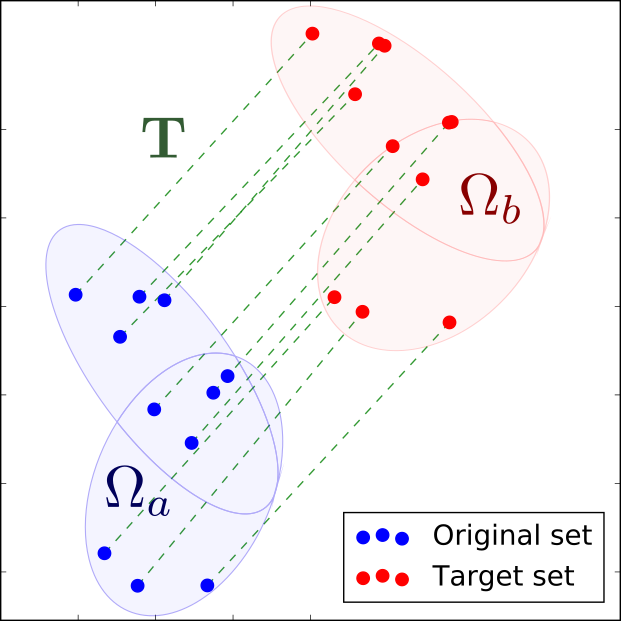
\includegraphics[height=1.4in]{6.matching/img/one}
        \caption{{\scriptsize Original \& target datasets}}
        \label{fig:otprob_a}
    \end{subfigure}%
    ~ 
    \begin{subfigure}[t]{0.32\textwidth}
        \centering
        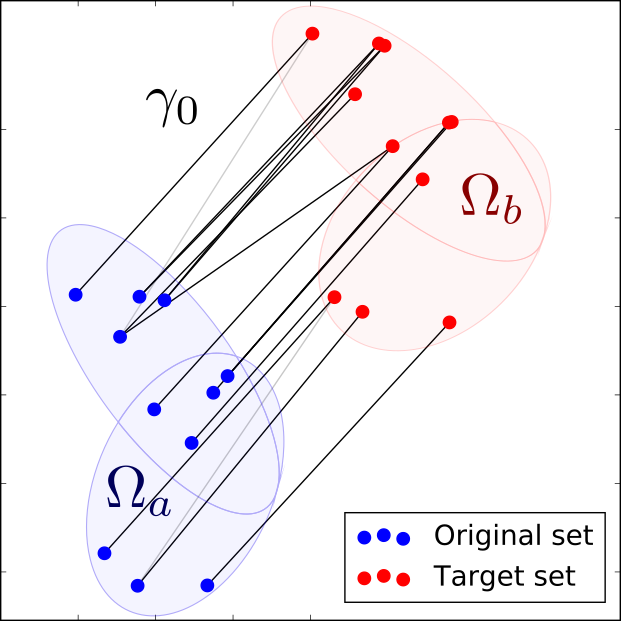
\includegraphics[height=1.4in]{6.matching/img/two}
        \caption{{\scriptsize Computed transport plan}}
        \label{fig:otprob_b}
    \end{subfigure}
    ~
    \begin{subfigure}[t]{0.32\textwidth}
        \centering
        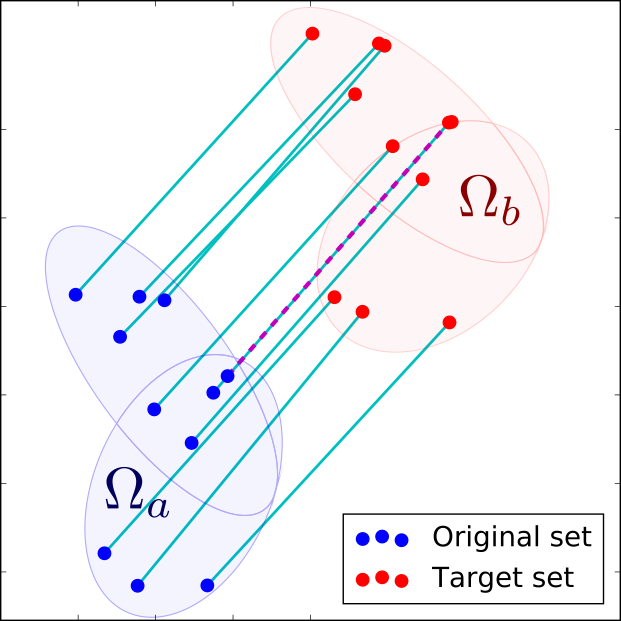
\includegraphics[height=1.4in]{6.matching/img/three}
        \caption{{\scriptsize Matching}}
        \label{fig:otprob_c}
    \end{subfigure}
    \caption{{\footnotesize A 2-d example of using OT to compute the matching between two different datasets. On the left we show the original and target datasets. The real matchings are displayed as green dashed edges. In the middle, the edge densities represent the values of the computed coupling $\gamma_0$, which denote the amount of mass that is exchanged between vectors $x_i^a$ and $x_j^b$. On the right, we see the recovered matching. The blue edges represent the correct matchings, while the red dotted edges represent the incorrect ones.}}
    \label{fig:otprob}
\end{figure*}

\begin{equation}
\gamma_0 = \argmin_{\gamma \in \mathcal{B}} \textnormal{~} \langle \gamma,C \rangle_F + \lambda \sum_{i,j} \gamma(i,j) \textnormal{~log~} \gamma(i,j)
\end{equation}
The matrix $C$, where $C(i,j) = \Vert x^a_i - x^b_j \Vert^2_2$, represents the cost of moving probability mass from location $x^a_j$ to location $x^b_i$, in terms of their squared Euclidean distance. The rightmost term is a regularization term based on the negative entropy of $\gamma$ allows us to solve this optimization problem using the Sinkhorn-Knopp algorithm~\cite{cuturi_sh} which improves the computation time.

Matrix $\gamma_0$ contains information about the exchange of probability mass between the vectors of $X^a$ and $X^b$. By construction, this exchange depends on the selected cost function. The choice of the squared euclidean distance is motivated both by the fact that it renders the optimization problem convex and because it will allow the parcels to be matched according to the vicinity of their feature vectors. Hence, the origin feature vectors will distribute their corresponding probability mass to the target feature vectors that are closest to them. Consequently, we define $\hat{\mathbf{T}}:\Omega^a \rightarrow \Omega^b$ as $\hat{\mathbf{T}}(x^a_i) = x^b_{\hat{j}}$ where $\hat{j} = \argmax_{j} \gamma_0(i,j)$. Therefore, $i$ will be matched to the parcel $\hat{j}$ that it sent the most mass to.

\subsection{Matching Parcels Based on Dissimilarity Between Features}
\label{sec:others}

% We define the three measures that we compare against our method. 
Let $d(x^a_i,x^b_j)$ be some dissimilarity measure between the elements of $X^a$ and $X^b$. Then, we say that parcel $i$ matches parcel $j$ if $\argmin_k d(x^a_i,x^b_k) = j$. We compare three dissimilarity measures against our method.
% ${d_e(x^a_i,x^b_j) = \lVert x^a_i - x^b_j \rVert_2}$, 
% ${d_c(x^a_i,x^b_j) =  1 - \{x^a_i\cdot x^b_j/\lVert x^a_i\rVert_2 \lVert x^b_j \rVert_2\}}$, and $d_{KL}(x^a_i,x^b_j) = \sum_{l=1}^d \tilde{x}^a_i(l) \log\{\tilde{x}^a_i(l)/\tilde{x}^b_j(l)\}$.
% \begin{equation*}
% \displaystyle
% d_e(x^a_i,x^b_j) = \lVert x^a_i - x^b_j \rVert_2
% \textnormal{,~~}
% d_c(x^a_i,x^b_j) =  1 - \frac{x^a_i\cdot x^b_j}{\lVert x^a_i\rVert_2 \lVert x^b_j \rVert_2}
% \textnormal{,~~and}
% \end{equation*}
% \begin{equation*}
% d_{KL}(x^a_i,x^b_j) = \sum_{l=1}^d \tilde{x}^a_i(l) \log\frac{\tilde{x}^a_i(l)}{\tilde{x}^b_j(l)}.
% \end{equation*}
First, we use the Euclidean distance, which  can be interpreted as matching
the parcel $i$ to the parcel $j$ whose feature vector $x^b_j$ is the closest
to $x^a_i$. Then, we use the cosine similarity, which is minimized when two
feature vectors are colinear. Lastly, we use the Kullback-Leibler divergence,
which measures the difference between two probability distributions in terms
of their relative entropy. Note that we need to convert our vectors into
probability vectors in order to evaluate $d_{KL}$. 

% We therefore normalize each feature vector $x$ such that $\tilde{x} = \frac{x}{\rVert x \lVert_\infty}$, thus $\sum_{l=1}^d \tilde{x}(l) = 1$, where $\tilde{x}(l)$ is the $l$-th coordinate of $\tilde{x}$.

\section{Experiments and Results}

\subsection{Data and Preprocessing}
\label{sec:fingerprint}
For this work we randomly selected 20 subjects from the S500 group of the Human
Connectome Project (HCP), all preprocessed with the HCP minimum
pipeline~\cite{Glasser2013}. Fiber orientation distributions functions where
computed using spherical constrained deconvolution with a spherical harmonic
order of 8. Probabilistic tractography was then performed using 1000 seeds per
vertex of the cortical mesh provided with the HCP data. For each subject, we
computed a connectivity matrix by counting the number of streamlines that
connect each pair of vertices of the cortical mesh. Each row in the matrix is
a vertex connectivity vector, representing the probability that a connection
exists between a surface vertex and the rest of the surface's vertices.
%\subsection{Computing a parcel's connectivity fingerprint}

Given a whole brain cortical parcellation, we compute the connectivity fingerprint
of each parcel by averaging the connectivity fingerprint of its vertices. Because
the mesh's vertices are coregistered across subjects~\cite{Glasser2013}, we are
able to compare the connectivity fingerprints across subjects. The criterion to
compute the parcel matching between two subjects is the similarity between
connectivity fingerprints. That is, we match two parcels if they are connected
to the rest of the brain in a similar manner. Due to the distance bias that
occurs in tractography, a parcel tends to be highly connected to the vertices
that compose it. To prevent the matching to be influenced by this bias, we
disconnect each parcel from its own vertices.

%The main advantages of using this public data base are the following. First, each subject possess a dense mesh representing their cortical surface, which we use to create seed-points for tractography. Then, all the mesh's vertices are coregistered across subjects, a property that allows us to compare connectivity fingerprints across subjects. Additionally, each subject possess the Desikan Atlas~\cite{Desikan2006} parcellation already computed over their cortical mesh. Finally, for each cortical mesh, there are also different z-score maps representing the response to different stimuli obtained with functional MRI (fMRI)~\cite{Barch2013}. These z-score maps are used to compute a functional parcellation for each subject.
 
\subsection{Matching Parcels}
\label{sec:matching}
In this section we evaluate the performance of our method by comparing it to the methods presented in Section~\ref{sec:others}. For each experiment we compute parcel matchings between all possible pairs of connectivity matrices. To quantify the result of each technique, we compute the accuracy in terms of percentage of correctly matched parcels per pairwise matching.

\subsubsection{Matching parcels with synthetic fingerprints.}

In this first experiment, we test the feasibility of our method by generating parcels with synthetic connectivity fingerprints and matching them. We start by generating a connectivity matrix $M$ using probabilistic Constrained Spherical Deconvolution based tractography to use as ground truth. Our ground truth matrix is a square matrix that represents the connectivity between the 64 parcels of the Desikan atlas in one subject of the HCP dataset. Each coefficient $M(i,j) = \theta_{ij}$ is the parameter of a random variable that follows a Bernoulli distribution $X_{ij} ~ B(\theta_{ij})$. This variable $X_{ij}$ represents the probability of a connection existing between the parcels $i$ and $j$. 
Using $M$, we generate 20 synthetic matrices in such a way that the coefficients of each synthetic connectivity matrix are random variables that follow a binomial distribution $X(i,j) \sim B(p=M(i,j),n)$. 
By doing this we simulate doing tractography for various values of the number $n$ of particles. Figure~\ref{fig:synth} shows the performance of each method as a function of $n$.  


%To this date, no mathematical model has been found for the variability in extrinsic connectivity across subjects \cite{Paquette2016}. Therefore, we test our method in synthetic connectivity matrices created using 3 different methods. In each method, we simulate 20 connectivity matrices starting from a connectivity matrix $M \in R^{64 \times 64}$ between the parcels of the Desikan atlas, derived from probabilistic tractography. Each coefficient $M(i,j) = \theta_{ij}$ of the connectivity matrix is the parameters of a random variable that follows a Bernoulli distribution $X_{ij} ~ B(\theta_{ij})$. This variable $X_{ij}$ represents the probability of a connection existing between the parcel $i$ and $j$.

%In the second one, we follow a noise model similar to the one proposed by Paquette et al. \cite{Paquette2016} and generate synthetic connectivity matrices by adding multiplicative Gaussian noise on each row of $M$. In particular, the $i$-th row of each synthetic matrix $M'$ is equal to the inner product ${M'(i) = \langle M(i),X_i \rangle}$, where $X_i \sim \mathcal{N}(a_i\mathbf{1}_{64},\sigma)$, $\mathbf{1}_{64}$ is a $64$-dimensional vector of ones, and $a_i \sim \mathcal{N}(0,1)$.
%Finally, in the third experiment we generate synthetic connectivity matrices using the logistic random effects model presented in Gallardo et al. (2017). Each synthetic matrix $M'$ comes from the model $logit(M') = logit(M) + \Gamma$ where $\Gamma \sim N(0, \sigma \mathbf{I})$ is normally distributed noise and $\mathbf{I}$ is the identity matrix. That is, we add additive noise in the logit space.


%We show the performance of the first technique as a function of the number of realizations $n$, i.e., the number of simulated particles.
%The performance of the other two technique are displayed as a function of the standard deviation of the noise.

\begin{figure*}[t!]
    \centering
    \begin{subfigure}[t]{0.52\textwidth}
        \centering
        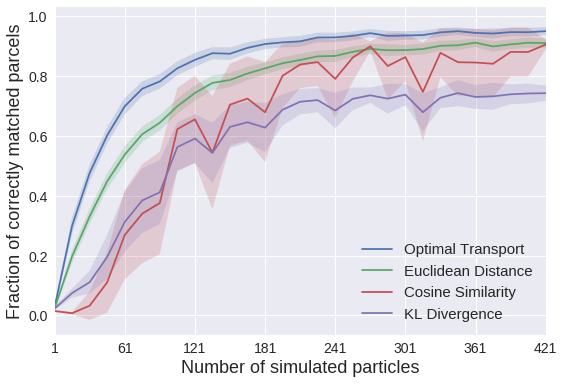
\includegraphics[height=1.7in]{6.matching/img/synthetic}
        \caption{{\scriptsize Synthetic data}}
        \label{fig:synth}
    \end{subfigure}%
    ~ 
    \begin{subfigure}[t]{0.52\textwidth}
        \centering
        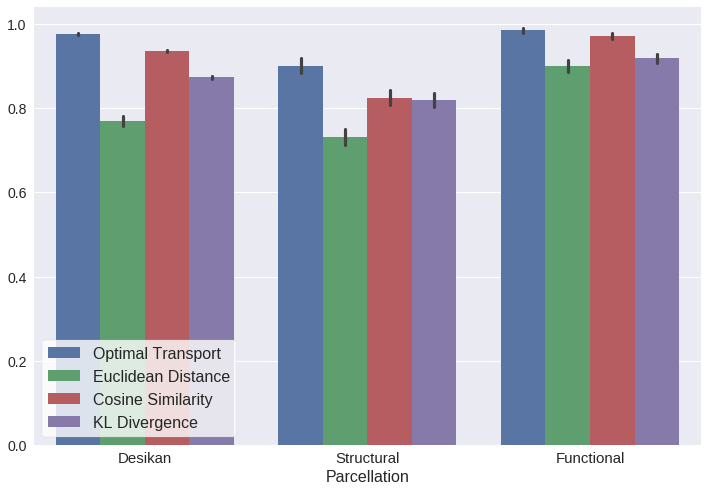
\includegraphics[height=1.7in]{6.matching/img/real}
        \caption{{\scriptsize Real data}}
        \label{fig:real}
    \end{subfigure}
    \caption{Proportion of parcels correctly matched by each method (see section~\ref{sec:others}) when matching: (a) synthetic connectivity fingerprints and (b) connectivity fingerprints of a cortical parcellation, for three different parcellations (as described in section~\ref{sec:matching}). OT always performs significantly better.}
    \label{fig:results}
\end{figure*}

\subsubsection{Matching parcels of the Desikan Atlas.}
For each subject, we compute the connectivity fingerprint of each parcel in their Desikan atlas as explained in Section \ref{sec:fingerprint}. When matching parcels across subjects, Figure~\ref{fig:real} shows that on average OT achieves an accuracy of 98\%$\pm$2\%, followed by cosine similarity (94\%$\pm$3\%), KL divergence (87\%$\pm$4\%), and finally Euclidean distance (77\%$\pm$11\%).

\subsubsection{Matching parcels created using functional criteria.}
Each subject in the HCP dataset possesses z-score maps representing responses to different stimuli obtained with functional MRI (fMRI)~\cite{Barch2013}. We derive parcels for each subject from the responses to motor (hand, foot and tongue movement) and visual stimuli (faces vs shape recognition). We do so by keeping only the vertices whose z-score is in the top 35\%.
Figure \ref{fig:real} shows that OT performs best with an average of 98\%$\pm$6\%. The cosine similarity, KL divergence, and Euclidean distance achieve average accuracies of 97\%$\pm$6\%, 92\%$\pm$10\%, and 90\%$\pm$13\% respectively.

\subsubsection{Matching parcels created using structural criteria.}
For each subject, we first mask their Lateral Occipital Gyrus using the Desikan atlas. Then, we divide it into 3 parcels using the structural based parcellation technique of Gallardo et al.~\cite{Gallardo2017a}. Once more, we can see on Figure \ref{fig:real} that optimal transport has the highest average accuracy, equal to 92\%$\pm$16\%. It is followed by the cosine similarity, the KL divergence, and the Euclidean distance, whose average accuracies equal 85\%$\pm$17\%, 84\%$\pm$17\%, and 75\%$\pm$17\%

\section{Discussion}
In this work we proposed a method to match parcels across subjects based on the
connectivity fingerprint of a parcel. 

We tested our method with four different experiments. In the first experiment
our technique correctly matched connectivity fingerprints created in a synthetic
way. Specifically, each entry in a fingerprint was sampled from a Binomial
distribution, whose parameter was chosen as the corresponding value of a
ground truth connectivity matrix. This can be thought as a simulation of the
process of tracking in tractography with different number of streamlines.
%This choice of simulation was motivated by the results in Paquette et al. \cite{Paquette2006} which shows that neither additive nor multiplicative noise are adequate cross-subject variability models.

Our second experiment shows that we can correctly match parcels of the Desikan
atlas across subjects with a 98\% of correct matches. The parcels of the Desikan
atlas are known to have high spatial coherence and consistent connectivity
profiles across subjects \cite{DeReus2013}. We therefore use this experiment
as a reference point to benchmark our technique.
The last two experiments show that our technique can match parcels generated
with a same criteria, even when they have some spatial variability across-subjects.
The first experiment uses parcels created from the functional response to specific
motor and visual stimuli, known to be strongly linked to functional
connectivity \cite{Osher2016, Penfield1954}. The second one, parcels created
from the structural parcellation of the Lateral Occipital Gyrus, a structure
documented to have a consistent structural division \cite{ThiebautdeSchotten2016, Gallardo2017a}. 

It's important to notice that our technique achieved more than a 90\% of correct
matches in every experiment with real data. Given that we used 20 subjects, this
represents a total of 20x19=380 cross-subject matches. In the case of the Desikan
atlas, which possesses 64 parcels, this translates into a total of 24320 matches,
from which 98\% where correctly matched. Furthermore, when tested with a paired
t-test to compare the number of correct matches, our method always performs
significantly better than the other three ($p<10^{-256}$).

% The fact that OT transport performs well can also imply the kind of
% transformation which occurs between the connectivity fingerprints of two
%cross-subject parcellations. 

\section{Conclusion}
In this chapter, we proposed a novel parcel matching method based on Optimal
Transport. We showed that our technique outperforms state-of-the-art matching
techniques in three different baseline scenarios.

Both this chapter and the previous one are based on the fact that we can
estimate brain connectivity. However, some brain pathologies can disrupt
the white matter, hampering the estimation of brain connectivity. In
the following chapter, we will introduce a technique to infer which
tracts are affected by a pathology, even when is not possible to use
tractography.



\chapterbib

    \chapter{Inferring the Localization of White-Matter Tracts using Diffusion Driven Label Fusion}

\section{Overview}
White matter pathologies such as tumors or traumatic brain injury disrupt the
structure of white matter. These disruptions hamper the inference of affected
pathways using tractography. A way to overcome this is to use a label fusion
technique. Label fusion aims to infer the localization of the brain structure
of a subject from its localization in a group of control subjects. The most
common technique is known as the voting rule \cite{voting}, where a structure
is said to be present in a voxel if it's present in the majority of the voting
subjects. Furthermore, this can be improved by weighting each vote by the
similarity between the T1 of each voting subject and the subject to be inferred.
However, these techniques only relay in the spatial localization of the structures.
In this work, we introduce a way to weight the vote of each subject based on
how the voted pathway is supported by the test subject's diffusion data. This
is, if the diffusion data of the test subject is consistent with the direction
of the voted pathway, the vote has a higher weight. We show that adding dMRI to
the label fusion process achieves a similar number of true positives than the
voting technique, with a 60\% less of false positives. However, this incurs in
a trade-off of a 40\% false negatives.

\section{Introduction}

White matter pathologies such as tumors or traumatic brain injury disrupt the
structure of white matter. These disruptions hamper the inference of affected
pathways using tractography. Furthermore, for some pathologies as tumors or
edemas, estimating brain pathways using tractography becomes impossible [cite].
For such pathologies, it's not possible to use Diffusion Magnetic Resonance
Imaging (dMRI) to tract within or around the lesion. Given the nature of the
lesions, the tracking results in interrupted or erroneous tracts. This situation
makes hard to infer which pathways are directly affect by the pathology. One
possible way to overcome this issue, is by aggregating spatial information
from other subjects in order to infer the affected tracts. Assuming we know the
location of a set of tracts in the brains of a group of healthy subjects, we
could register them to the brain of our patient and use a label fusion technique.
Label fusion is a family of techniques that aims to infer the localization of the
 brain structure of a subject from its localization in a group of control subjects.
One well known technique within this family is Majority Voting [cite]. Given a
specific location, each subject is said to "vote" for one label. The inferred
label for that location will be the one with more votes. For example, when
labeling a volume, each voxel receives the label voted by the majority of the
control subjects.

Majority Voting is simple to implement and has been demonstrated to yield
accurate segmentations [reference]. However, this technique is blind both to
registration problems and anatomical variability between subjects. To overcome
this, it has been propose to weight the vote of each subject by some measure of
 similarity between the patient and the subject [cite]. The underlying
intuition is the choosing of labels should be driven by those subjects who
resemble the most to the one being labeled. The practical advantages of various
strategies based on this idea have recently been demonstrated [6-sabuncu].

The techniques described so far relay only on anatomical information, not taking 
into account the structure of white matter. In the case of white matter pathways,
the presence of a path constrains the brownian motion in the brain, which can be
measured by dMRI. In this work, we introduce a new label fusion technique that,
taking advantage of dMRI, weights the vote of each subject based on how the voted
pathway is supported by the test subject's diffusion data. This is, if the
diffusion data of the test subject is consistent with the direction of the voted
pathway, the vote has a higher weight. Our technique also allows to work with
crossing tracts, by modeling multiple labels per voxel.

We validate our technique in 13 subjects of the Human Connectome Project (HCP).
For each subject, we infer the location of 18 left hemisphere tracts using
whole-brain tractography and an implementation of the white matter query language
(WMQL). We use this results as ground truth to compare against inferring the
tracts from using the other 12 subjects with our proposed technique and Majority
Voting. Our results show that adding dMRI to the label fusion process achieves a
similar number of true positives than Majority Voting, with a 60\% less of
false positives, incurring in a trade-off of a 40\% false negatives.

\section{Methods}

Our label fusion technique takes advantage of dMRI to weight the vote of each
subject. The vote for a specific label gets a higher weight if it's supported
by the diffusion data of the subject being labeled. In this section, we first
start explaining the concept of Orientation Density Function of diffusion in
dMRI and tract directionality. Then, we present how to use these concepts to
compute the weights of each vote.

\subsection{Estimating an Orientation Density Function from dMRI Data}
A dMRI image is composed by many volumes, each one linked to an acquisition
direction. Each value in these volumes represents the intensity of diffusion
in that point of the brain for the direction linked to the volume. By fitting
the diffusion information of a voxel in a Constrained Spherical Deconvolution
model, it's possible to estimate a orientation density function (ODF) over a
sphere. Needs more explanation.

\subsection{Estimating an Orientation Density Function from Streamlines}
Given a tract expressed as set of streamlines, assuming they don't have sharp
turns we can estimate their main directionality on a voxel by looking at its
entry and exit points. For each pair of entry and exit points we can compute a
direction, and from this set of directions, we can compute a ODF over a sphere,
expressing the distributions of directions for that voxel. Explain ACGD.

% Since we also want to estimate directionality from tracts, we introduce the concept of acgd
\subsection{Label fusion}
In the previous section we presented how to compute and ODF from dMRI data and
how to estimate the ODF from a tract in a voxel. Now, we introduce the Majority
Voting technique and our improvement using dMRI.

\subsubsection{Majority Voting}
Let $labels = \{l_i\}, \forall_i l_i \in N$ be the set of labels representing
tracts and grey matter structures in one hemisphere. Let ${L_s}, s \in S$
represent the labeling of a set of subjects $S$, where each 
$L_s \in labels^{v\times v}$ is a 3D volume represeting the labeling of a
specific subject. Majority Voting [Rohlfing et al. (2004)] infers the label of
each voxel $x$ in the test subject ($L(x)$) by computing:

\begin{equation}
\label{eq:mvoting}
\begin{aligned}
    \hat L(x) = \argmax_{l \in labels} \sum_{s\in S} p(L(x) = l | L_s(x)),\\
    \text{where} \\
    p(L(x) = l | L_s(x)) =
    \begin{cases}
        1,& \text{if } L_s(x) = l \\
        0,& \text{otherwise}
    \end{cases}
\end{aligned}
\end{equation}

In this case, it's said that each train subject votes for a label per voxel,
and the label with the most amount of votes is assigned to the test subject's
voxel.

\subsubsection{Diffusion based label fusion}
We want to introduce a weight to these votes, taking into account how well the
tract can explain the underlying Diffusion data of our test subject. In
particular, we want to the Orientation Distribution Function (ODF) of our
test subject's diffusion. This is, we want to profit of the fact that we know
how the water particles are moving in its brain, following the underlying tracts.
As explained in section X, in a given voxel, we can compute the main
directionality of the tract $l$ of the train subject $s$ and the ODF of our
test subject's diffusion. To see if the tract are aligned with the
directionality of the voted tract we proposed the following model:

\begin{equation}
\label{eq:argmax}
\hat L(x) = \argmax_{l \in labels} \sum_{s\in S} p(L(x) = l ; L_s(x)) p(D(x) ; D_{sl}(x)),
\end{equation}
where
\begin{equation}
\label{eq:peaks}
p(P(x) ; D_{sl}(x)) = <ODF(x), ODF_sl(x)>.
\end{equation}

In our model, the first term remains the same as in the voting scheme.
Our second term, $p(D(x) | D_{sl}(x))$ express the probability
of seeying the ODF that we found in our test subject, given that the real
tract passing by is the one voted by the test subject. We compute this
probability as in [REFERENCE], by computing the inner product between the
two ODFs. The ODFs need to be first normalized in order for <ODF, ODF> = 1.

In the case of multi-label, we can combine the info of directions in a same acgd.
This allows us to better compute the real label when there are fibers crossing
inside of a voxel.
For each voxel in the white-matter of our test subject, we select the label
with the highest summation of weighted votes. 

\section{Experiments and Results}

In the previous section we presented how to add Diffusion weighted information
to the process of Mayority Voting in order to improve the multi-atlas technique.
Now, we present experiments, both in synthetic and real data, showing that
our technique achieves better results than Mayority Voting.

\subsection{Data and Preprocessing}
We randomly selected 13 subjects from the HCP500 dataset from the Human
Connectome Project. For each subject, we computed whole-brain tractography
using each voxel in the white-matter as a seed and simulating 8 particles per
seed [REF]. We extracted the main tracts from the left hemisphere tractogram
(18 tracts in total) using the implementation of the white-matter query
language (WMQL),(Wasserman et al. 2016). For each pair of subjects, we
registered they tracts to each others brain.

\subsection{Assessing goodness of the technique in synthetic data}
The dwi of TEST has one tract. We have two types of subjects, ST who votes for
a tract, and S0 who votes for no tracts. ST starts with a completely aligned
tract, and we go rotation it until 90 deg. Then, we compute the weight of
each vote. The proportion between them, tells us how many subjects we need to
get either one or the other label. We show that, when we have subjects voting
for the right tract, their weight go up, allowing to only 30\% of them to win.
But when the tract is not aligned, then they lose, except if they're the 70\%.
In between.. stuff.
But, when the GT is NO-TRACT, we always need more than 60\% of the people.
Something similar happens with crossing, I hope.
This is better than the 50\% of voting.

\subsection{Assessing goodness of the techniques in real data}
To assess the "goodness" of our technique we made a leave-one-out
cross-validation. At each step, we selected one of the subjects as test and 
used the rest as train subjects. Using the registered tracts of the train
subjects, we computed parcellations using both the voting rule and our technique.
Since we also have the tracts of each test subject, we compute a 'ground truth'
parcellation of they white matter. Finally, we computed the confusion matrix of
both the Majority Voting and our technique. A confusion matrix is a matrix of 
size labels by labels where the entry (i,j) is the number of times the label in
the ground truth was i and the technique labeled j. Table 1 shows that our
proposed achieves a similar number of false negatives while obtaining a 64\%
less of false positives in average. This incurs on a trade-off of having 39\%
more false negatives and 18\% less true positives in average, underlying that
our technique a more conservative.\\

\subsection{Simulating Lesions in the White-Matter}
To test how our technique would behave in a injured brain, we simulate a tumor in the white matter of one of our subjects. We place the tumor to interrupt the ILF. We do so by selecting a set of neighboring voxels where the ILF passes by, and mix their signal with diffusion signal from random voxels in the ventricles. This is, for each selected voxel $x$ in the brain, we chose a random voxel $v$ in the ventricle and mix their signals:
$$S(x) = S(x)(1-\alpha) + S(v)\alpha, \alpha \in [0,1]$$.
Since the ventricles are regions filled with cerebrospinal fluid (CSF), they diffusion is approximately isotropic. We compute for which values of $\alpha$ WMQL stops being able to detect the ILF, and for which values our technique stops being able to detecting it. Since the Major Voting does not rely on diffusion data, this experiment does not affect the results obtained in the previous experiment for Major Voting.
WMQL stops detecting the ILF at... and our technique stops detecting it in the voxels at .... 

\subsection{Discussion}
We want to infer the position of tracts in the white matter.
Since we do not have many subjects, we cannot relay on Deep Learning techniques.
We decide to use Label Fusion techniques.
Some people showed that Mayority Voting works well for this things.
The problem is that majority voting relies only on the spatial location.
Problems of registration.
We introduce a new way to take into account the diffusion information.
This makes a lot of sense, since we are trying to infer tracts, and the 
diffusion data is related to the underlying tracts.
In synthetic data, we show that our technique is much better than
majority voting, specially when the tracts align correctly with the
underlying diffusion. It also works like charm, when the tracts are completely
missaligned with the diffusion. In other cases, is as good as majority voting.
In real data, this is reflected, by showing that diffusion voting is more
conservative. WMM lessions.

\subsection{Conclusions}
In this work we presented a labeling fusion technique that relies on dMRI data
to infer the localization of white-matter tracts. The results show that our
technique is more conservative than the voting rule, which is desired when
studying pathologies, at the cost of having more false negatives.

\subsubsection*{Table}

\begin{table}[]
\centering
\caption{Confusion matrix for both techniques and the ratio between them}
\label{my-label}
\begin{tabular}{|l||l|l||l|l||l|l|}
\hline
      & \multicolumn{2}{c||}{Diffusion} & \multicolumn{2}{c||}{Voting} &  \multicolumn{2}{|c|}{Diffusion / Voting} \\ 
      \hline
            & Background  & Tract & Background  & Tract     & Background  & Tract \\
      \hline
Background  & 3658350     & 11849 & 3568123     & 24619     & 1.00        & 0.48   \\
      \hline
Tract       & 27932       & 2592  & 17050       & 3163      & 1.64        & 0.82   \\
\hline
\end{tabular}
\end{table}

Figure 1. Outline of our technique. We extract the main white-matter tracts using WMQL, register them to the 'test' subject and then compute a voting rule weighted by diffusion information. For each voxel $x$ in the 'test' subject, we select the label $l$ that maximizes equation \ref{eq:argmax}, where S is the set of 'train' subjects, $t$ is the 'test' subject; $L_i(x)$ is the label of voxel $x$ for the subject $i$; $P$ are the principal directions of diffusion in the 'test' subject and $D_{sl}(x)$ are the directions of tract $l$ in the voxel $x$ of the 'train' subject $s$.

    %\chapter{Groupwise Structural Parcellation of the Whole Cortex: A Logistic Random Effects Model Based Approach}
%
%
\section{Overview}
So far in this thesis we have introduced the necessary concepts in neuroanatomy;
non-invasive imaging techniques to study the brain, and brain parcellation. In
the first chapter we explained the importance of brain connectivity and its
relation to brain function. On the second chapter, we explained how to estimate
brain connectivity and brain function in a non-invasive way. The third chapter
showed the ongoing effort to find new and relevant ways to divide the brain,
in order to improve the way to study it. In particular, all of the parcellations
based on structural connectivity are computationally expensive; need tuning of
several parameters or rely on ad-hoc constraints. Furthermore, none of these 
methods present a model for the cortical extrinsic connectivity of the cortex.
In this chapter, we propose a parsimonious model for the extrinsic connectivity
and an efficient parceling technique based on clustering of tractograms. 
Our technique allows the creation of single subject and groupwise parcellations
of the whole cortex. We show that our technique creates parcellations in
agreement with anatomical, structural and functional parcellations extant in 
the literature.

This work has been published in the journal Neuroimage \cite{Gallardo2017}
%
\section{Introduction}
%
The human brain is arranged in areas based on criteria such as cytoarchitecture,
functional specialization or axonal connectivity~\citep{Brodmann1909, Thirion2014,
ThiebautdeSchotten2016}. Parceling the cortex into such areas and 
characterizing their interaction is key to understanding how the brain works.
Nowadays it is accepted that axonal connectivity plays a fundamental role in the
interaction between brain regions~\citep{Schmahmann2006}. Moreover, current theories
hold that long-range physical connections trough axonal bundles,
namely \textit{extrinsic connectivity}, are strongly related to brain function, for example,
this has been shown in macaques~\citep{Passingham2002}. Therefore, understanding
how the cortex is arranged based on its extrinsic connectivity can
provide key information in unraveling the internal organization of the brain.

Diffusion MRI (dMRI) enables the in vivo exploration of extrinsic connectivity 
and other aspects of white matter anatomy on the brain. However, in using diffusion
MRI to infer long-distance connectivity, several challenges arise. A primary issue
is the spatial resolution of diffusion imaging: it is several
orders of magnitude coarser than axonal diameters (millimeters vs.
micrometers)~\citep{VanEssen2014}, making hard to infer some brain pathways.
In addition, there is as yet no quantitative
measure of the strength of connections from diffusion~\citep{Jbabdi2013}.
Given these general limitations, obtaining a cortical parcellation based on
extrinsic connectivity remains challenging~\citep{VanEssen2014, Jbabdi2013}.
Moreover, most current parceling
techniques compute either single-subject or groupwise parcellations.
Single-subject techniques work by refining other
parcellations~\citep{Clarkson2010}, which introduces a bias in the resulting
parcellation; parceling only part of the 
cortex~\citep{Lefranc2016, Roca2009, ThiebautdeSchotten2014, ThiebautdeSchotten2016}
or using ad-hoc metrics to compare extrinsic connectivity~\citep{Moreno-Dominguez2014}.
Meanwhile, existing groupwise methods rely on average connectivity
profiles~\citep{Clarkson2010, Roca2010}, which prevents obtaining single
subject parcellations; seek a matching across subjects after independent
parcellations~\citep{Moreno-Dominguez2014}, relying on possible noisy results,
or need fine tuning of parameters, as the expected number of clusters to
find~\citep{Paristot2015}.

\begin{figure*}
    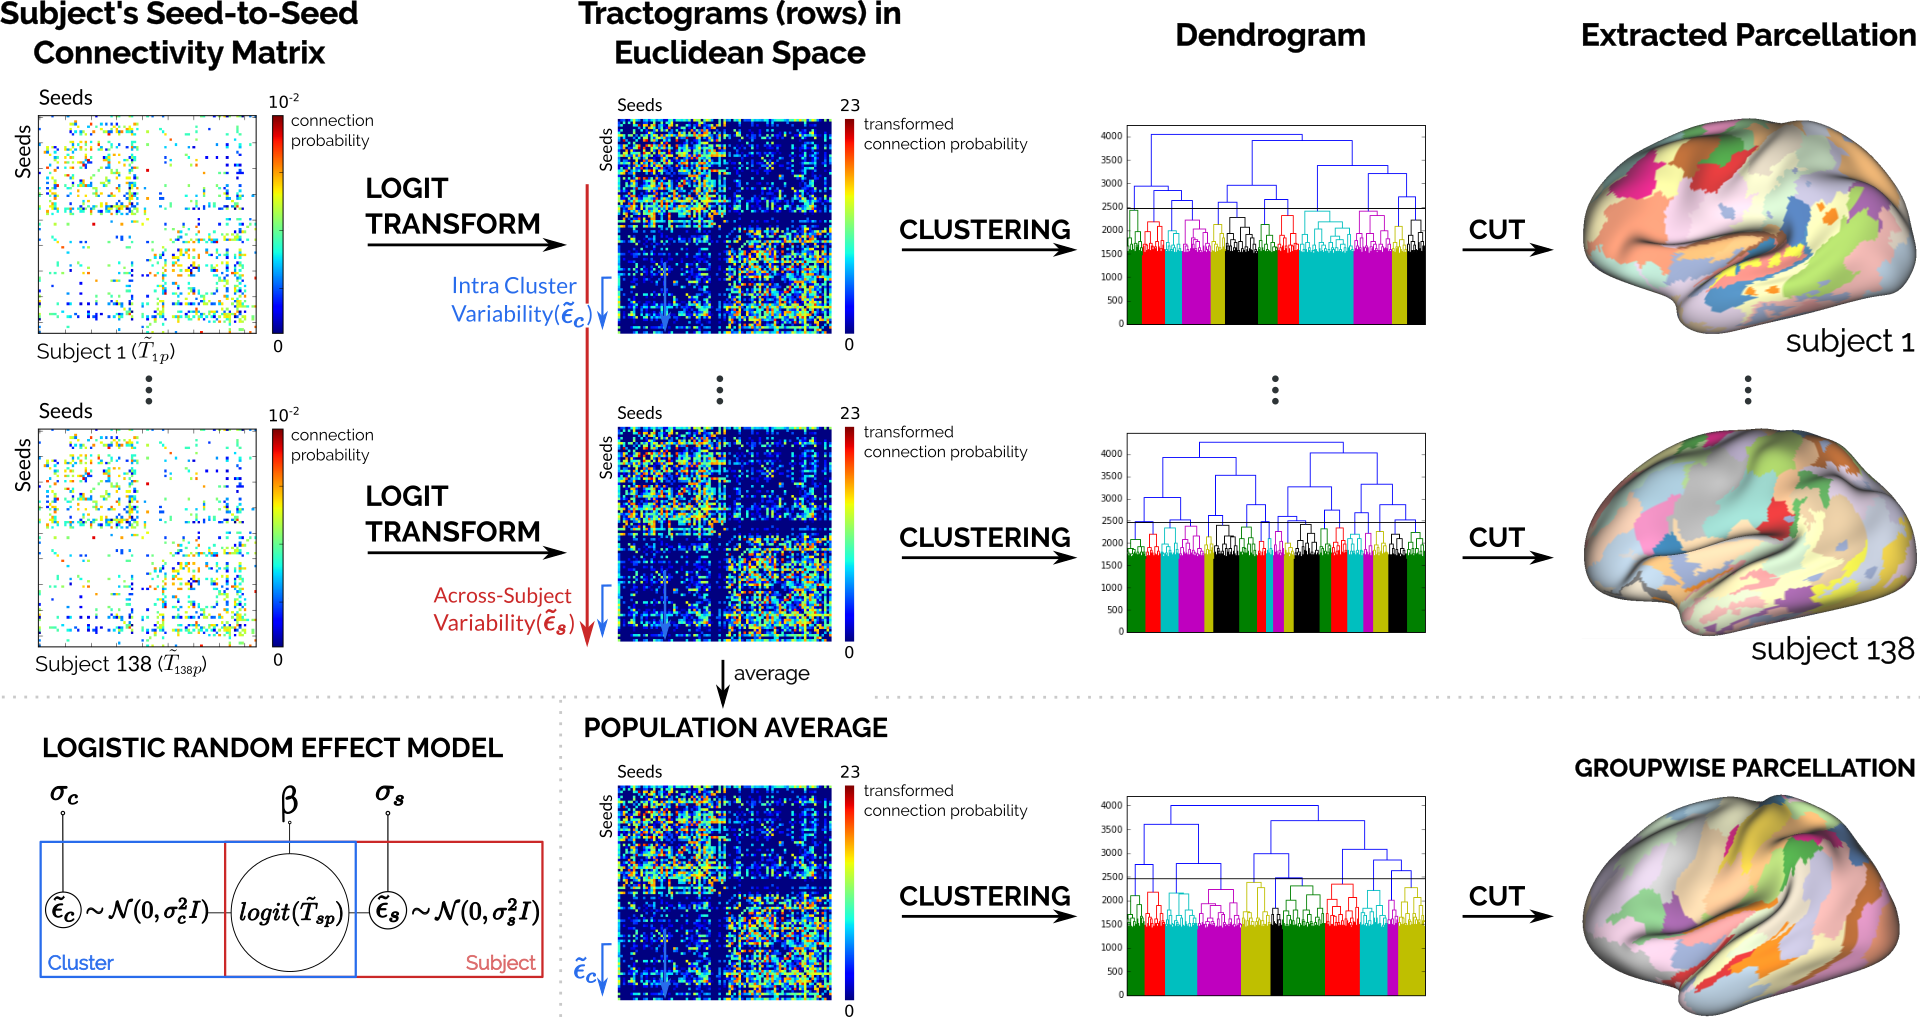
\includegraphics[width=\textwidth]{5.structural_clustering/img/summary.png}
    \caption{Lower left corner: graphical model of the linear relationship
             between the tractogram of a subject $s$ for a seed $p$ ($\tilde T_{sp}$); and the intra-cluster
             ($\tilde \epsilon_c$) and across-subject ($\tilde \epsilon_s$) variability of the seed's patch. We transform the tractograms 
             into a Euclidean space while explicitly accounting for the variability. This allows us to use well known clustering techniques and 
             compress different levels of granularities for a same parcellation
             in a dendrogram.}
    \label{fig:summary}
\end{figure*}

In this work, we present a parsimonious model for the cortical
connectivity alongside an efficient parceling technique based on it. We summarize
both contributions in Fig.~\ref{fig:summary}. Our model assumes that the cortex is
divided in patches of homogeneous extrinsic connectivity. That is, nearby
neurons in the cortex share approximately the same long-range physical
connections, we call this the \textit{local coherence criterion}. Our assumption
is based on histological results in the macaque brain~\citep{Schmahmann2006}.
Inspired by statistical models for clustered data~\citep{Pendergast1996}, our model
accounts for the variability in the axonal connections of neurons within a patch
and for variability in patch boundaries across subjects. Our parceling technique
allows us to create single subject and groupwise parcellations of the whole
cortex in agreement with extant parcellations.

We validate our technique by taking advantage of data available from the Human
Connectome Project (HCP). Using our technique, we compute single subject and a
groupwise parcellations. In this work we will focus on the groupwise case. For
results of our method on the single-subject case please refer to \citet{Gallardo2017}.
Here, we first assess the consistency of our groupwise parceling technique by
comparing the groupwise parcellations of three disjoint groups of 46 subjects
from the HCP. We also show that our technique computes a similar parcellation to
the one obtained by \citet{ThiebautdeSchotten2016} when parceling only the frontal
cortex. Later, to test the functional specialization of our frontal lobe parcels,
we use a data-base of meta-analysis of fMRI studies \citep{Yarkoni2011}, as in
\citet{ThiebautdeSchotten2016}. After, we show that our groupwise parcels subdivide
some well-known anatomical structures by comparing our results against Desikan's
atlas~\citep{Desikan2006}. Also, we show the functional specialization of some of
our parcels by comparing against results from \citet{Glasser2013}. Finally, we
compare our groupwise parcellation of 138 subjects against the multi-modal
parcellation of \citet{Glasser2016}. We show that, while the parcellations
boundaries differ, our parcels show similar or better functional specialization,
specially for motor related tasks.

This work is organized as follows: In the Methods section we present our
model for cortical connectivity and frame tractography within our model. Also,
we present both our single-subject and groupwise case methodologies to parcellate
the cortex. In the Experiments and Results section we present our results on HCP
data. We then discuss our results and position ourselves with respect to the state
of the art in the Discussion section. Finally, in the last section we provide our
conclusions.
%
\section{Methods}
%
\subsection{Cortical Connectivity Model and Tractography}
\label{sec:cortical_model}
Our model assumes that the cortex is divided in clusters of homogeneous extrinsic
connectivity. That is, nearby neurons in the cortex share approximately the same
long-ranged physical connections, we call this the \textit{local coherence criterion}.
Our assumption is based on histological results in the macaque brain~\citep{Schmahmann2006}.
As in clustered data models in statistics~\citep{Pendergast1996}, we allow
intra-cluster and across-subject variability in the connectivity. We formalize this concept as:
%
\begin{equation}
    \label{eq:notation}
    K = \bigcup_{i=1}^k K_i , \forall_{1 \leq i,j \leq k}, i \neq j \rightarrow K_i \cap K_j = \emptyset \land \on{conn}(K_i) \neq \on{conn}(K_j)
\end{equation}
%
where the set of points on the cortex $K$ is the disjoint union
of each cluster $K_i$ and $\on{conn}(\cdot)$ is the extrinsic connectivity
fingerprint of a cluster. We will make the notion of variability explicit in eq. 
\ref{eq:tractogram_rv}. In this work, the connectivity fingerprint of a seed-point
in the brain is a binary vector denoting to which other seed-points it is
connected through axonal bundles. That is, the physical connections of a point
$p \in K_i$ in the brain are represented by its connectivity fingerprint
$\on{conn}(p) = \on{conn}(K_i)$.

Currently, the most common tool for estimating the extrinsic connectivity
fingerprint of a point in vivo is probabilistic tractography~\citep{Jbabdi2013}.
Given a seed-point in the brain, probabilistic tractography creates a
\textit{tractogram}: an image where each voxel is valued with its probability
of being connected to the seed through axonal bundles. One way of calculating
these probabilities is with a Monte Carlo procedure, simulating the random walk
of water particles through the white matter~\citep{Behrens2003a}. Each one of
these paths is known as a streamline. If we model these streamlines as Bernoulli
trials, where we get a value for the connection from our seed with other points
(1 if they connected by the streamline, 0 if not)~\citep{Behrens2003a}, then, we
can model the tractogram of the subject $s$ in the seed-point $p$ as:
%
\begin{equation}
    \label{eq:tractogram}
    T_{sp} = 
      [P(\rv C_{spi}=1)]_{1 \leq i \leq n} =
      [\theta_{spi}]_{1 \leq i \leq n}, ~~ \rv C_{spi} \sim \on{Bernoulli}(\theta_{spi})
    \enspace,
\end{equation}
%
where $\rv C_{spi}$ is a Bernoulli random variable\footnote{For the sake of
clarity we denote all random variables with a tilde, e.g. $\rv C$.} 
representing ``the point $p$ of the subject $s$ is connected to the voxel $i$".
Each Bernoulli's parameter ($\theta_{spi}$) represents the probability of being
connected, and is estimated as the proportion of success in the Bernoulli
trials of each seed.

To formulate the tractogram in accordance to our hypothesis of cortical
connectivity, we model it as a vector of random variables. In our
model, each element in a tractogram comes from a random variable depending on
the point's cluster along with its intra-cluster and across-subject variability:
\begin{equation}
    \label{eq:tractogram_rv}
        p \in K_c \rightarrow
        \rv T_{sp} = 
        [P(\rv C_{spi}=1 | \on{conn}(K_c), ~\rv \epsilon_{ci}, ~\rv \epsilon_{si})]_{1 \leq i \leq n}
        \enspace ,
\end{equation}
%
in this case, the point $p$ belongs to the cluster $c$;  $\rv \epsilon_{ci}$ 
represents the intra-cluster variability and $\rv \epsilon_{si}$ represents the
across-subject variability for the connectivity to voxel $i$ in the cluster $c$. 

Since each $\rv C_{spi}$ follows a Bernoulli distribution (Eq. \ref{eq:tractogram})
it is difficult to find an explicit formulation for 
$P(\rv C_{spi} = 1 | \on{conn}(K_c),~\rv \epsilon_{ci}, ~\rv \epsilon_{si})$ 
accounting for the variabilities. For this, we use the generalized linear
model (GLM) theory. In this theory, the data is assumed to follow a linear form
after being transformed with an appropriate link function~\citep{McCullagh1989}.
Using the following notation abuse:
%
\begin{equation}
    \label{eq:not_abuse}
    \on{logit}(\rv T_{sp}) \triangleq  [\on{logit}(P(\rv C_{spi}=1 | \on{conn}(K_c), ~\rv \epsilon_{ci}, ~\rv \epsilon_{si})]_{1  \leq i \leq n},
\end{equation}
\noindent
%
we derive from GLM a logistic random-effects model~\citep{Pendergast1996} for
each point $p$:
%
\begin{equation}
    \label{eq:ran_eff_model}
    \on{logit}(\rv T_{sp}) = \beta_{c} + \rv \epsilon_{c} + \rv \epsilon_{s} \in \R^n,
    \quad
    ~ \rv \epsilon_{c} \sim \N(\vec 0, \sigma_c^2 Id),
    ~ \rv \epsilon_{s} \sim \N(\vec 0, \sigma_s^2 Id),
\end{equation}
%
where $\epsilon_{c}$ and $\epsilon_{s}$ represent the intra-cluster and 
across-subject variability respectively. According to GLM theory 
$\beta_c \in \R^n$ is the extrinsic connectivity fingerprint of cluster $K_c$
transformed: 
%
\begin{equation}
    \on{logit}^{-1}(\beta_c) = E(\rv T_{sp}) = \on{conn}(K_c) \enspace.
\end{equation}

The choice of logit as link function is based on the work of \citet{Pohl2007}.
In their work, \citet{Pohl2007} show that logit function's codomain is a
Euclidean space, which allows us to transform and manipulate the tractograms 
in a well-known space.
%
\subsection{Single Subject and Groupwise Parceling Methodologies}
\label{sec:parceling_methodologies}
%
In the previous section, we hypothesized that the cortex is divided in
clusters with homogeneous extrinsic connectivity, alongside intra-cluster and
across-subject variability. In using
the previous hypothesis, it is important to remark that we don't have a priori
knowledge of the cluster's location or their variability. But, thanks to the
proposed logistic random effects model, we formulated the problem of finding
these clusters as a well-known clustering problem. This is because, after
transforming the tractograms with the logit function as in eq.~\ref{eq:not_abuse}
they will be in a Euclidean space~\citep{Pohl2007}. Even more, eq.~\ref{eq:ran_eff_model}
states that the transformed tractograms come from a mixture of Gaussian 
distributions, e.g. it is a Gaussian mixture model.

To solve the Gaussian mixture model and find the clusters, we use a modified
Agglomerative Hierarchical Clustering (AHC) algorithm. This was inspired by the
method of \citet{Moreno-Dominguez2014}. To enforce the local coherence
criterion we also modify the algorithm to accept one parameter: the minimum size
of the resulting clusters. Clusters smaller than this size are merged with
neighbors, i.e. physically close clusters in the cortex. As we are working in
a Euclidean space, we use Ward's Hierarchical Clustering
method~\citep{WardJr.1963}. 
This method creates clusters with minimum within-cluster variance.
The method's result is a dendrogram: a structure that comprises different levels of
granularity for the same parcellation. This allows us to explore different
parcellation granularities by choosing cutting criteria, without the need of
recomputing each time.

The main advantage of the model we proposed in this work is that it
allows us to create a groupwise parcellation using linear operations. Assuming
direct seed correspondence across subjects, as in the HCP data set, our model
lets us remove the subject variability of each seed's tractogram by calculating
the expected value across subjects:
%
\begin{equation}
    \label{eq:expected_subject}
    E_s(g(\rv T_{sp})) = E_s(\beta_{c} + \rv \epsilon_{c} + \rv \epsilon_{s}),
    = \beta_{c} + \rv \epsilon_{c} + E_s(\rv \epsilon_{s})
    = \beta_{c} + \rv \epsilon_{c}.
\end{equation}
% 
where the last equality is due to $E_s(\rv \epsilon_s)=0$
(Eq. \ref{eq:ran_eff_model}). Since in our model the variabilities are normally
distributed (Eq. \ref{eq:ran_eff_model}), we can estimate the expected value across
subjects by averaging a seed's tractograms across subjects. This allows us to create
population-representative tractograms for each seed free of across-subject 
variability, which then can be clustered to create a groupwise parcellation.
%
\section{Experiments and Results}
%
In the previous section we presented a model for the cortical extrinsic 
connectivity and a clustering technique to parcellate the whole brain. Our technique
allows us to create single subject and groupwise parcellations, encoded with
different levels of granularity in a dendrogram. Now, we show the results of
applying our technique over the HCP dataset. First, we explain how the 
preprocessing step of tractography was made. Then, we elaborate 
in detail how we applied our technique. Later, we show that our groupwise 
technique creates results consistent when parceling different groups. Also,
we show that our techniques creates parcels in accordance with those by 
\citet{ThiebautdeSchotten2016} when parceling only the frontal lobe. Then,
we present a proof-of-principle that our parcels are related to brain anatomy
and functional specialization. Most of the results in this section are focused
in the groupwise case, for further information on the single-subject technique
please refer to \citet{Gallardo2017}. Finally, we study the (dis)similarity
between our groupwise parcellation and that of \citet{Glasser2016}.
%
\subsection{Data and Preprocessing}
%
\subsubsection{Human Connectome Project Dataset}
A total of 138 subjects (65 males and 73 females, ages 31-35) were randomly 
selected from the group S500 of the Human Connectome Project (HCP). For
information on the acquisition protocols please refer to \citet{VanEssen2012}.
Every subject has been already preprocessed with the HCP minimum 
pipeline~\citep{Glasser2013}. Also, each subject's cortical surface is
coregistered and represented as a triangular mesh of approximately 32000
vertices per hemisphere~\citep{Glasser2013}. For each
vertex, the corresponding label from Desikan's Atlas is known~\citep{Desikan2006}.
Finally, the group S500 contains tfMRI information representing the average
response to functional stimuli in 100 unrelated subjects (U100)\citep{Barch2013}.
%
\subsubsection{Probabilistic Tractography}
To create the tractograms of each subject, we performed Constrained Spherical 
Deconvolution (CSD) based tractography~\citep{Tournier2004} from a dense set of
points in the cortex. Specifically, since each subject has a mesh representing
their gray-matter/white-matter interface~\citep{Glasser2013}, we used their
vertices as seeds to create tractograms. Vertices corresponding to the medial
wall were excluded. To avoid superficial cortico-cortical fibers~\citep{Reveley2015},
we shrank each of the 138 surfaces $2mm$ into the white matter. For each subject,
we fitted a CSD model~\citep{Tournier2004} to their diffusion data using Dipy
(version 0.11)~\citep{Garyfallidis2014} and created 5000 streamlines per seed-voxel
using the implementation of probabilistic tractography in Dipy. Later, we
created a tractogram as in (Eq. \ref{eq:tractogram}) by calculating for each
seed the fraction of they particles that visited other seed-voxel.
%
\subsection{Parceling Subjects From the Human Connectome Project}
After performing tractography, we applied our parceling technique over each
subject in our HCP sample. Specifically, we first transformed each tractogram 
with the logit function as in eq. \ref{eq:not_abuse}. Then,
we clustered the tractograms of each subject using the modified AHC algorithm
while imposing a minimum cluster size of $3mm^2$ in the finest granularity.
To retrieve parcellations from the resulting dendrogram we use the horizontal cut
method \citep{Murtagh2011, Moreno-Dominguez2014, Gallardo2017}. Two examples of
obtained single-subject parcellations at a granularity of 55 parcels are shown
in fig. \ref{fig:single_and_group}.
%
To create the groupwise parcellation, we took advantage of the vertex
correspondence across subjects in the HCP data set~\citep{Glasser2013}. After
transforming the tractograms with the logit transform, we computed the average
connectivity of each seed by averaging its tractograms across-subject. Then, we
computed the groupwise parcellation by clustering the averaged tractograms with our
proposed technique (sec. \ref{sec:parceling_methodologies}). The obtained groupwise 
parcellation at a granularity of 55 parcels is shown in fig.
\ref{fig:single_and_group}.
%
\begin{figure*}
    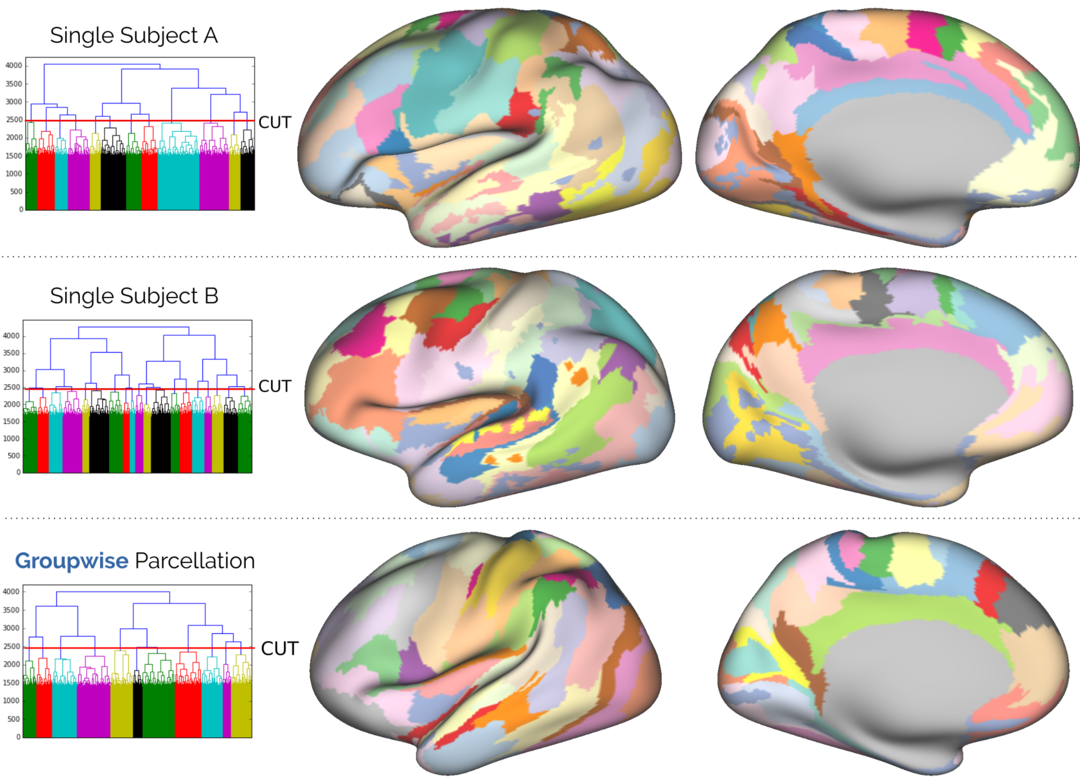
\includegraphics[width=\textwidth]{5.structural_clustering/img/single_and_group.png}
    \caption{Examples of two single-subject parcellations and the groupwise parcellations
    		 computed with our technique. All the parcellations shown have 55 parcels.
             The corresponding dendrogram for each case, along with the chosen cut height
             (red line) are shown. The groupwise parcellation
             is based on 138 subjects from the Human Connectome Project.}
    \label{fig:single_and_group}
\end{figure*}
%
\subsection{Groupwise Parcellation Technique Consistency}
To study the consistency of our technique, we randomly divided our HCP subject
sample 
in 3 disjoint groups, trying to maintain the same proportion of males and females
on each. The resulting groups had: 24 females, 22 males (group A); 23 females, 
23 males (group B) and 28 females, 18 males (group C). For each group we computed
their groupwise parcellation. The resulting parcellations at two different levels 
of granularity are shown in fig. \ref{fig:groups}.
%
\begin{figure*}
    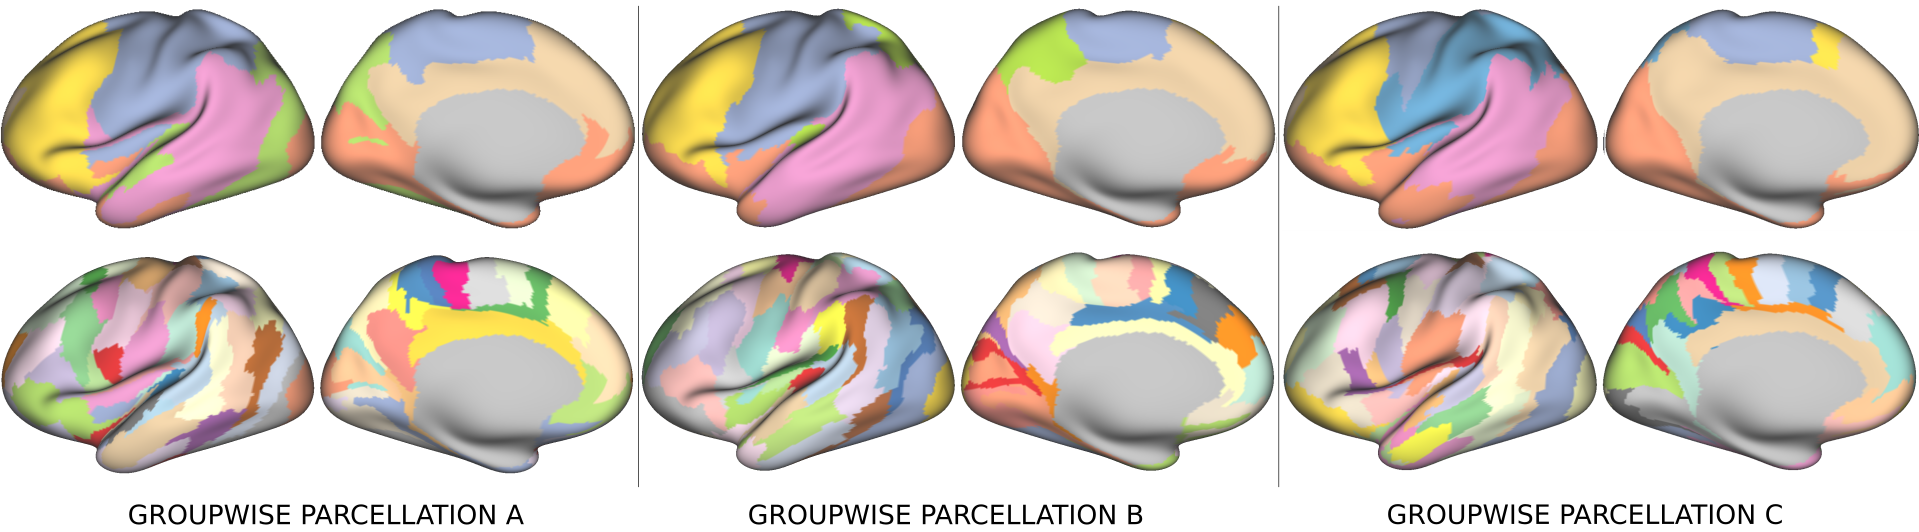
\includegraphics[width=\textwidth]{5.structural_clustering/img/groupwise_parcellations.png}
    \caption{Groupwise parcellations of 3 disjoint groups of 46 people each.
             We show results from the same dendrogram cut to get 6 parcels (upper)
             and 55 parcels (lower). Labels with best overlap in upper figures share
             the same color. Notice that there are two different shades of blue for 
             the group C.}
    \label{fig:groups}
\end{figure*}
%
To study the similarity between the obtained groupwise parcellations, we compared
them at different levels of granularity using the adjusted Rand
index~\citep{Hubert1985}. To have a baseline for the comparisons, we generated
random parcellations of the cortex and computed the similarity between them. 
We computed two types of random parcellations: The first one is an homogeneous
random parcellation with $n$ parcels, inspired in a method used by \citet{Paristot2015}. 
To compute it, we start by choosing $n$ starting points in the cortex, then, we
randomly expand each parcel
on the cortex. By comparing these random parcellations between them we compute 
the minimum obtainable Rand index by mere chance at each level of granularity. 
In the second type of random parcellation, 
we simulate the behavior of our technique. For this, we create a parcellation 
with $300$ parcels and then, we iteratively merge two parcels chosen at random until
all the parcels are merged in one. By comparing these random parcellations between
them we
obtain the minimum obtainable Rand index by a random Hierarchical Clustering
Algorithm. 
Examples of these random parcellations can be seen in Fig \ref{fig:fake_parcels}. 
The baselines presented in fig. \ref{fig:real_vs_fake} (yellow and violet lines)
were computed by comparing $1000$ of these random parcels at different levels
of granularity.
%
\begin{figure*}
    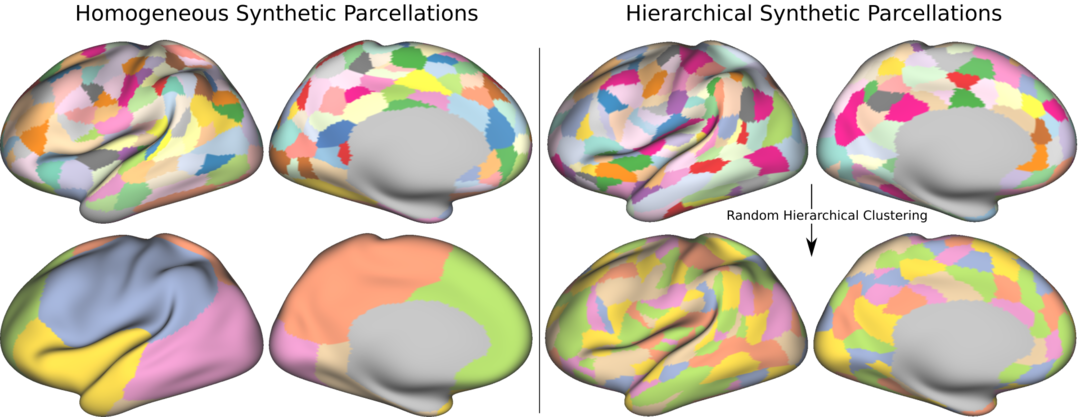
\includegraphics[width=\textwidth]{5.structural_clustering/img/fake_parcels.png}
    \caption{Examples of synthetic parcellations created to compute a baseline
             adjusted rand index. Parcellations on the left were created by 
             dividing the brain in a homogeneous way, inspired by the random
             parcellation presented in \citet{Paristot2015}. Parcellations on
             the right were created by randomly merging parcels of a coarse
             parcellation.}
    \label{fig:fake_parcels}
\end{figure*}
%
The result of comparing the groupwise parcellations of each group appear in
fig. \ref{fig:real_vs_fake}. The figure shows that the similarity between
our groupwise parcellations (lines red, green and blue) are significantly
higher than the baselines (violet and yellow). That is, the similarity
between our parcellations differs (for most cases) more than 3 standard 
deviations from the baselines' mean. Moreover, the similarity between our
results differs more
than 4 standard deviations from the comparison between synthetic hierarchical
parcels. This results show that our groupwise parceling technique creates
consistent parcellations.
%
\begin{figure*}
    \centering
    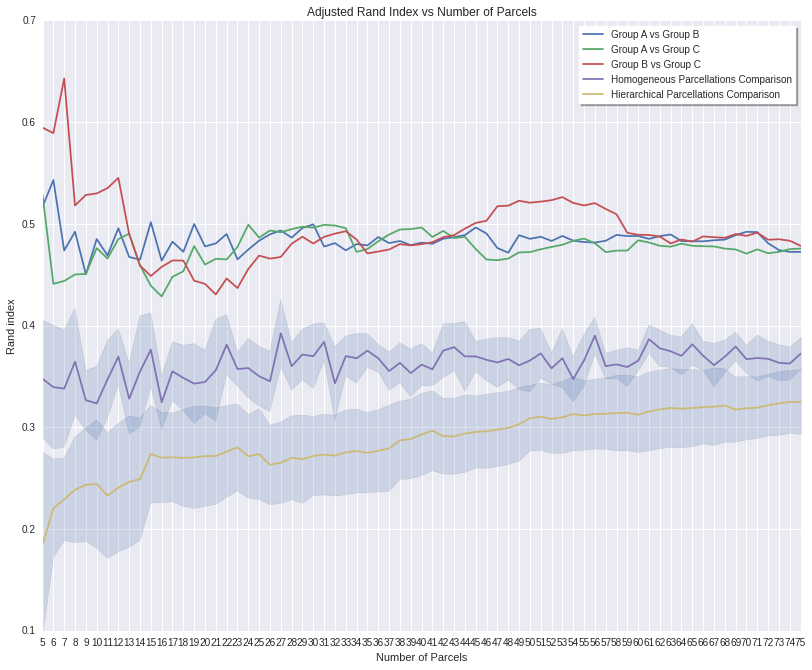
\includegraphics[width=\textwidth]{5.structural_clustering/img/real_vs_fake_parcellations.png}
    \caption{Adjusted Rand Index obtained when comparing: (red) Group A vs Group B;
             (blue) Group A vs Group C; (green) Group B vs Group C; (purple)
             Synthetic Homogeneous Parcels and (yellow) Synthetic hierarchical
             Parcels.}
    \label{fig:real_vs_fake}
\end{figure*}
%
\subsection{Relationship with a Frontal Lobe Parcellation}
Here we assess the agreement of our technique with an state-of-the-art extrinsic 
connectivity parceling technique. We do so by using our technique to parcellate 
the frontal lobe and compare our result against that of \citet{ThiebautdeSchotten2016}. 
In their work, \citet{ThiebautdeSchotten2016} use a principal component analysis (PCA)
statistical framework to parcellate the frontal lobe. They obtain a parcellation
with 12 parcels. Then, they show that each one of these parcels possess a functional
specialization by using the Decode tool\footnote{http://www.neurosynth.org/decode/}
from Neurosynth \citep{Yarkoni2011}. 
Thiebaut's parcellation is currently available in Neurovault \citep{Gorgolewski2016}
as an annotated volume\footnote{http://neurovault.org/collections/1597/}, registered
on the Colin27 template \citep{Holmes1996}. We downloaded this
parcellation and projected its parcels into a dense mesh representing the
cortex of the Colin27 template. The dense mesh had the same amount of vertices
as our chosen HCP subjects, and such vertices were coregistered with the
HCP subjects' cortical surfaces ones.

\begin{table*}[t]
\centering
\scalebox{0.9}{
  \begin{tabular}{@{}cccc@{}}
      \multicolumn{4}{c}{\textbf{Table 1. Correlation value reported (Neurosynth)}}  \\ \midrule
\textbf{Parcel} & \textbf{Term} & \textbf{$r$ (Thiebaut et al.)} & \textbf{$r$ (Ours)}\\
\textbf{1} & foot  & 0.267 & \textbf{0.319} \\
\textbf{2} & motor & 0.129 & \textbf{0.208} \\
\textbf{3} & eye field & 0.081& 0.048\\
\textbf{4} & speech production &0.077&\textbf{0.138}\\
\textbf{5} & pre sma &0.245&0.234\\
\textbf{6} & phonological &0.206&0.019\\
\textbf{7} & - &-&-\\
\textbf{8} & executive control & 0.049 & 0.042\\
\textbf{9} & - &-&-\\
\textbf{10}& semantic &0.178&\textbf{0.226}\\
\textbf{11}& social &0.137&0.110\\
\textbf{12}& semantic &0.139&0.086\\      \bottomrule
\end{tabular}}
% 
\vspace{0.3cm}
\caption*{Table 1. Spatial correlation value reported by Neurosynth for specific
                   terms in each parcel of \citet{ThiebautdeSchotten2016} and
                   for our parcels. Enumeration comes from figure~\ref{fig:frontal}.} 
\end{table*}

From the Desikan Atlas \citep{Desikan2006} of each of our HCP subjects, we
derived a groupwise mask for the frontal lobe. Then, we computed a groupwise 
parcellation with our technique, using only the tractograms in the mask. Figure
\ref{fig:frontal} shows both the parcellation downloaded from Neurovault
and our groupwise parcellation projected in the Colin template cortical surface.
The figure shows our parcellation with 10 parcels since this level of
granularity showed the best Rand index against the Thiebaut's parcellation.
The colors of each parcel in our groupwise parcellation were picked in base to
the position and amount of overlapping with the Thiebaut's parcels on the
surface. While the similarity according to the Rand index is not significantly
high ($0.4$), some visual similarity can be observed on the obtained parcellation,
particularly in the blue, yellow, orange and green parcels. Moreover, as shown in
table 1, our parcels show the same or even a higher level of functional
specialization when processed with Neurosynth.

\begin{figure*}
    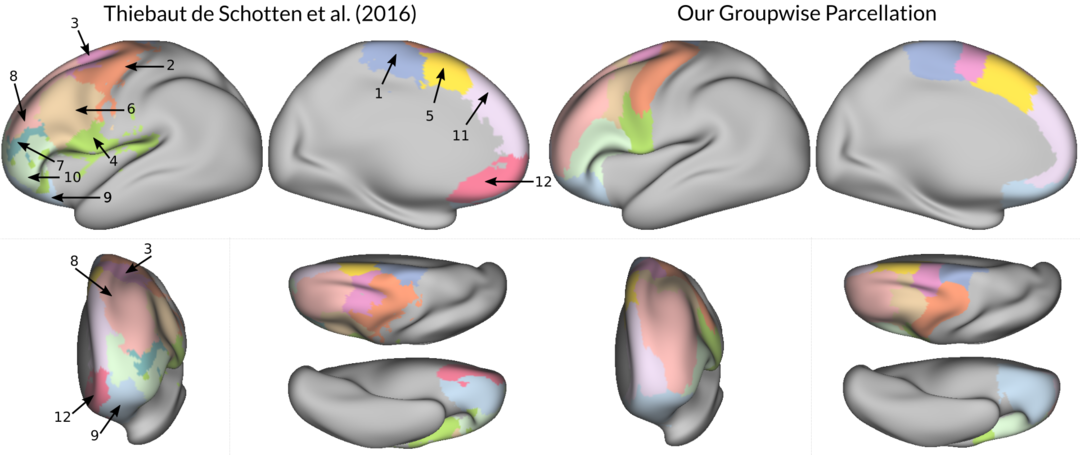
\includegraphics[width=\textwidth]{5.structural_clustering/img/frontal_lobe.png}
    \caption{\citet{ThiebautdeSchotten2016} parcellation (left) and our groupwise
    	     parcellation using only tractograms from the frontal lobe (right).
             Our parcels are colored after the parcel from \citet{ThiebautdeSchotten2016}
             with which they best overlap.}
    \label{fig:frontal}
\end{figure*}

To study the consistency of our result we computed the frontal lobe groupwise
parcellation in each of the 3 disjoint groups from the previous experiment. Figure~
\ref{fig:indices_by_lobe} shows the three obtained parcellation alongside
the Thiebaut's one. The obtained parcels show consistency, obtaining
an adjusted Rand index score of $0.61 \rpm 0.05$ between them. Finally, we
studied if the masking affected the clustering of the frontal lobe. To do so,
we applied the frontal lobe mask over a groupwise whole-brain parcellation of
the 138 subjects. The resulting frontal lobe parcellation contained 12 parcels.
This parcellation showed consistency with the one obtained by clustering only
the tractograms in the frontal lobe. More specifically, the adjusted Rand index
score between them was $0.65$. We repeated this procedure for the 3 disjoints
groups from the previous experiment. In each group, both frontal lobe parcellations
showed to be consistent, achieving an adjusted Rand index of $0.57 \rpm 0.04$.
%
\begin{figure*}
    \centering
    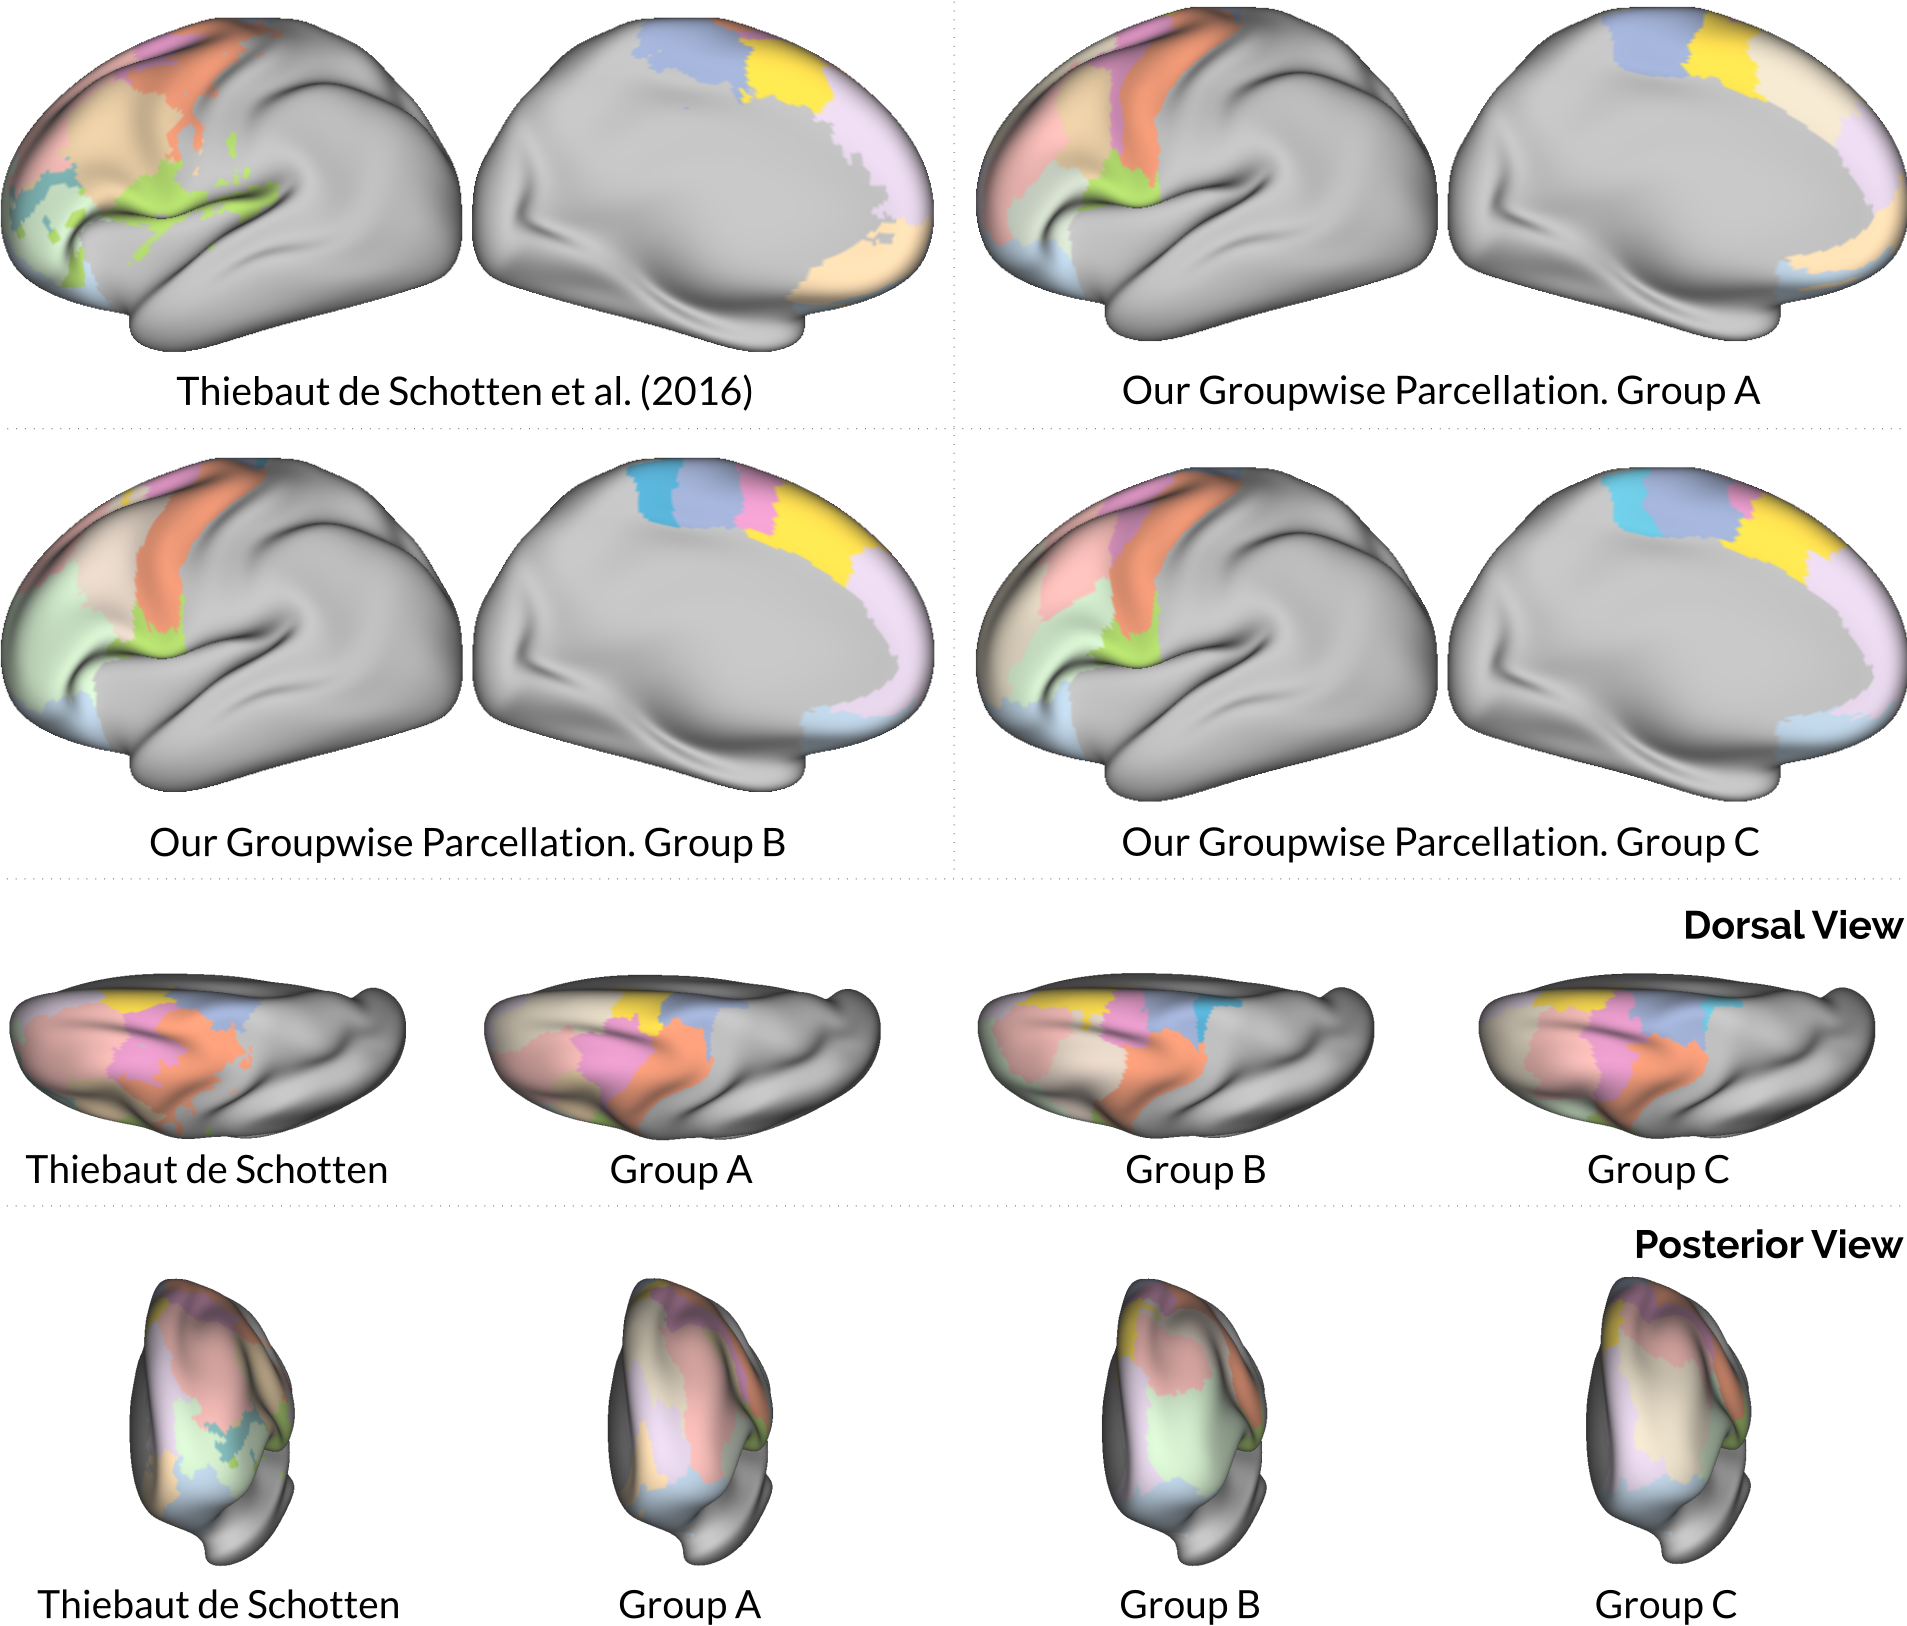
\includegraphics[width=\textwidth]{5.structural_clustering/img/3groups_frontal.png}
    \caption{\citet{ThiebautdeSchotten2016} parcellation (top-left) and our
    		 frontal lobe groupwise parcellations computed over 3 disjoint 
             groups of subjects. Our parcels are colored after the parcel from
             \citet{ThiebautdeSchotten2016} with which they best overlap.}
    \label{fig:indices_by_lobe}
\end{figure*}
%
\subsection{Anatomical Relationship and Functional Specialization of Our Parcels}
%
Here we present a proof of concept that our technique creates parcels within
anatomical boundaries and with functional meaning. To do so, first, we extracted
a parcellation with 55 parcels from the groupwise parcellation
computed from the 138 subjects. This was made to get a  parcellation with coarse
granularity while having at least the amount of 
parcels in the anatomical atlas of Desikan~\citep{Desikan2006} (36 parcels). We
compare this extracted parcellation against the Desikan Atlas and a functional
study made to every subject in the HCP~\citep{Glasser2013}.
%
\subsubsection{Relationship with Anatomical Boundaries}
%
\begin{figure*}
    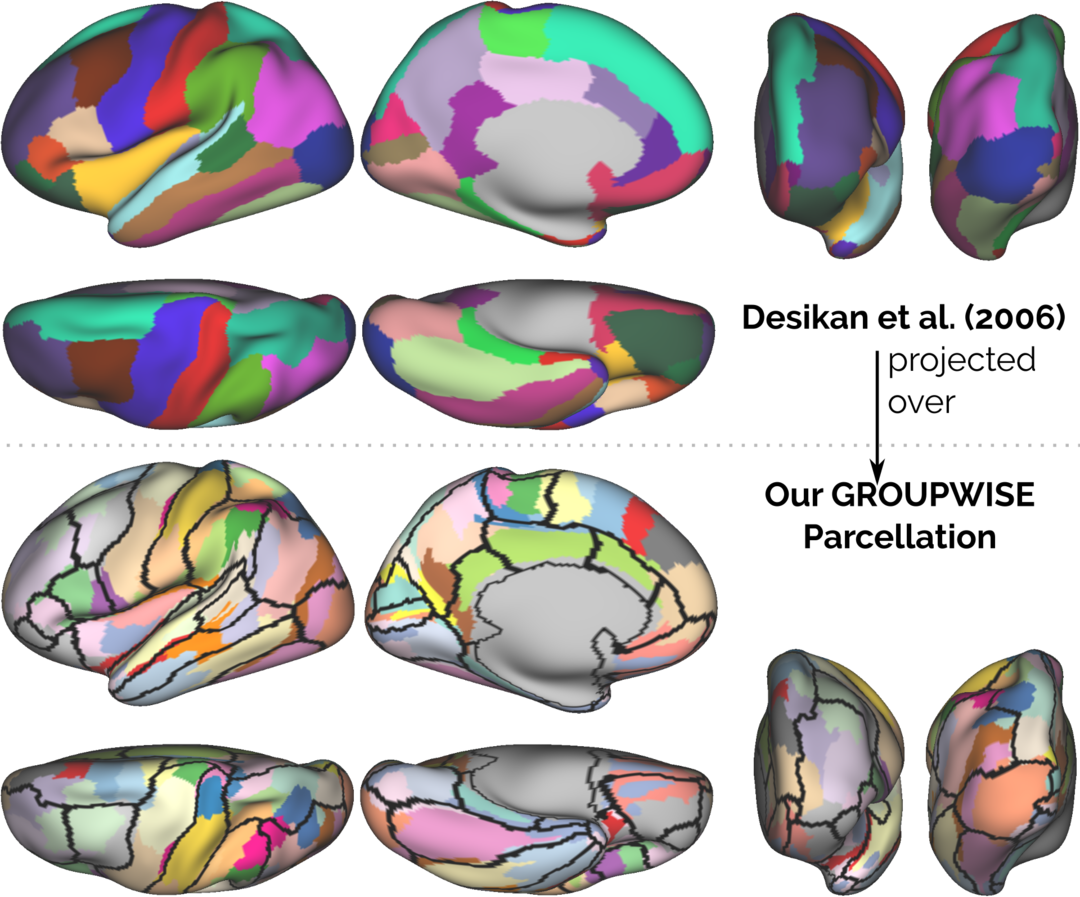
\includegraphics[width=\textwidth]{5.structural_clustering/img/anato.png}
    \caption{Relation between our pure extrinsic parcellation and the anatomical
             atlas of Desikan~\citep{Desikan2006}. Desikan atlas
             projected over the groupwise parcellation with 55 parcels.
             Insula; Cingulate; Lateral-Occipital; Fusiform; Superior Frontal;
             Lingual; Sensory and  Motor Cortex appear to be found.}
    \label{fig:anatomical_zoom}
\end{figure*}
%
To assess if some anatomical structures were present in the dendrogram and 
if our resulting parcels were subdividing them, we compared our extracted
parcellation with the Desikan atlas~\citep{Desikan2006}. To do so, we projected 
the Desikan regions over our parcels and then calculated: how many of our parcels
were contained by a anatomical region in more than a $90\%$, and which anatomical
regions were contained inside of one of our parcels. Using this criterion, the Insula; 
Cingulate; Lateral-Occipital; Fusiform; Superior Frontal; Lingual; Sensory and
Motor Cortex appear to be found as shown in Fig. \ref{fig:anatomical_zoom}.
%
\subsubsection{Functional Specialization.}
%
To study the relationship between our parcels and brain function, we projected our 
parcels over z-score maps representing responses to functional 
stimuli~\citep{Barch2013}. These maps are available as part of the HCP data, 
and represent the average activation of 100 subjects. In particular, we used
the maps related to 
the following tasks: right hand, foot and tongue movement; face, shape
recognition  and story categorization. For information on the functional tasks,
acquisition and processing of this data please refer to \citet{Barch2013}. 
Figure \ref{fig:function_motor} shows our parcels projected over contrasts
in motor tasks. In particular, our parcels are projected over the following
contrasts: tongue-average; hand movement-average and foot movement-average. 
Figure \ref{fig:function_cognition} shows our parcels projected over contrasts
in cognitive tasks: face-shape recognition; shape-face recognition and short-story
categorization. The figures show a good overlap between our parcels and the
regions with maximum activation of each task. In both figures the distribution
of z-scores inside of specific regions are shown as histograms. Further 
information about the z-score is present in tables 2 and 3. These tables show
that our parcels contain zero or few negatives values; that the mean of their
contained z-score is always positive and also, that many of those parcels 
enclose the maximum achievable z-score.

\begin{figure*}
    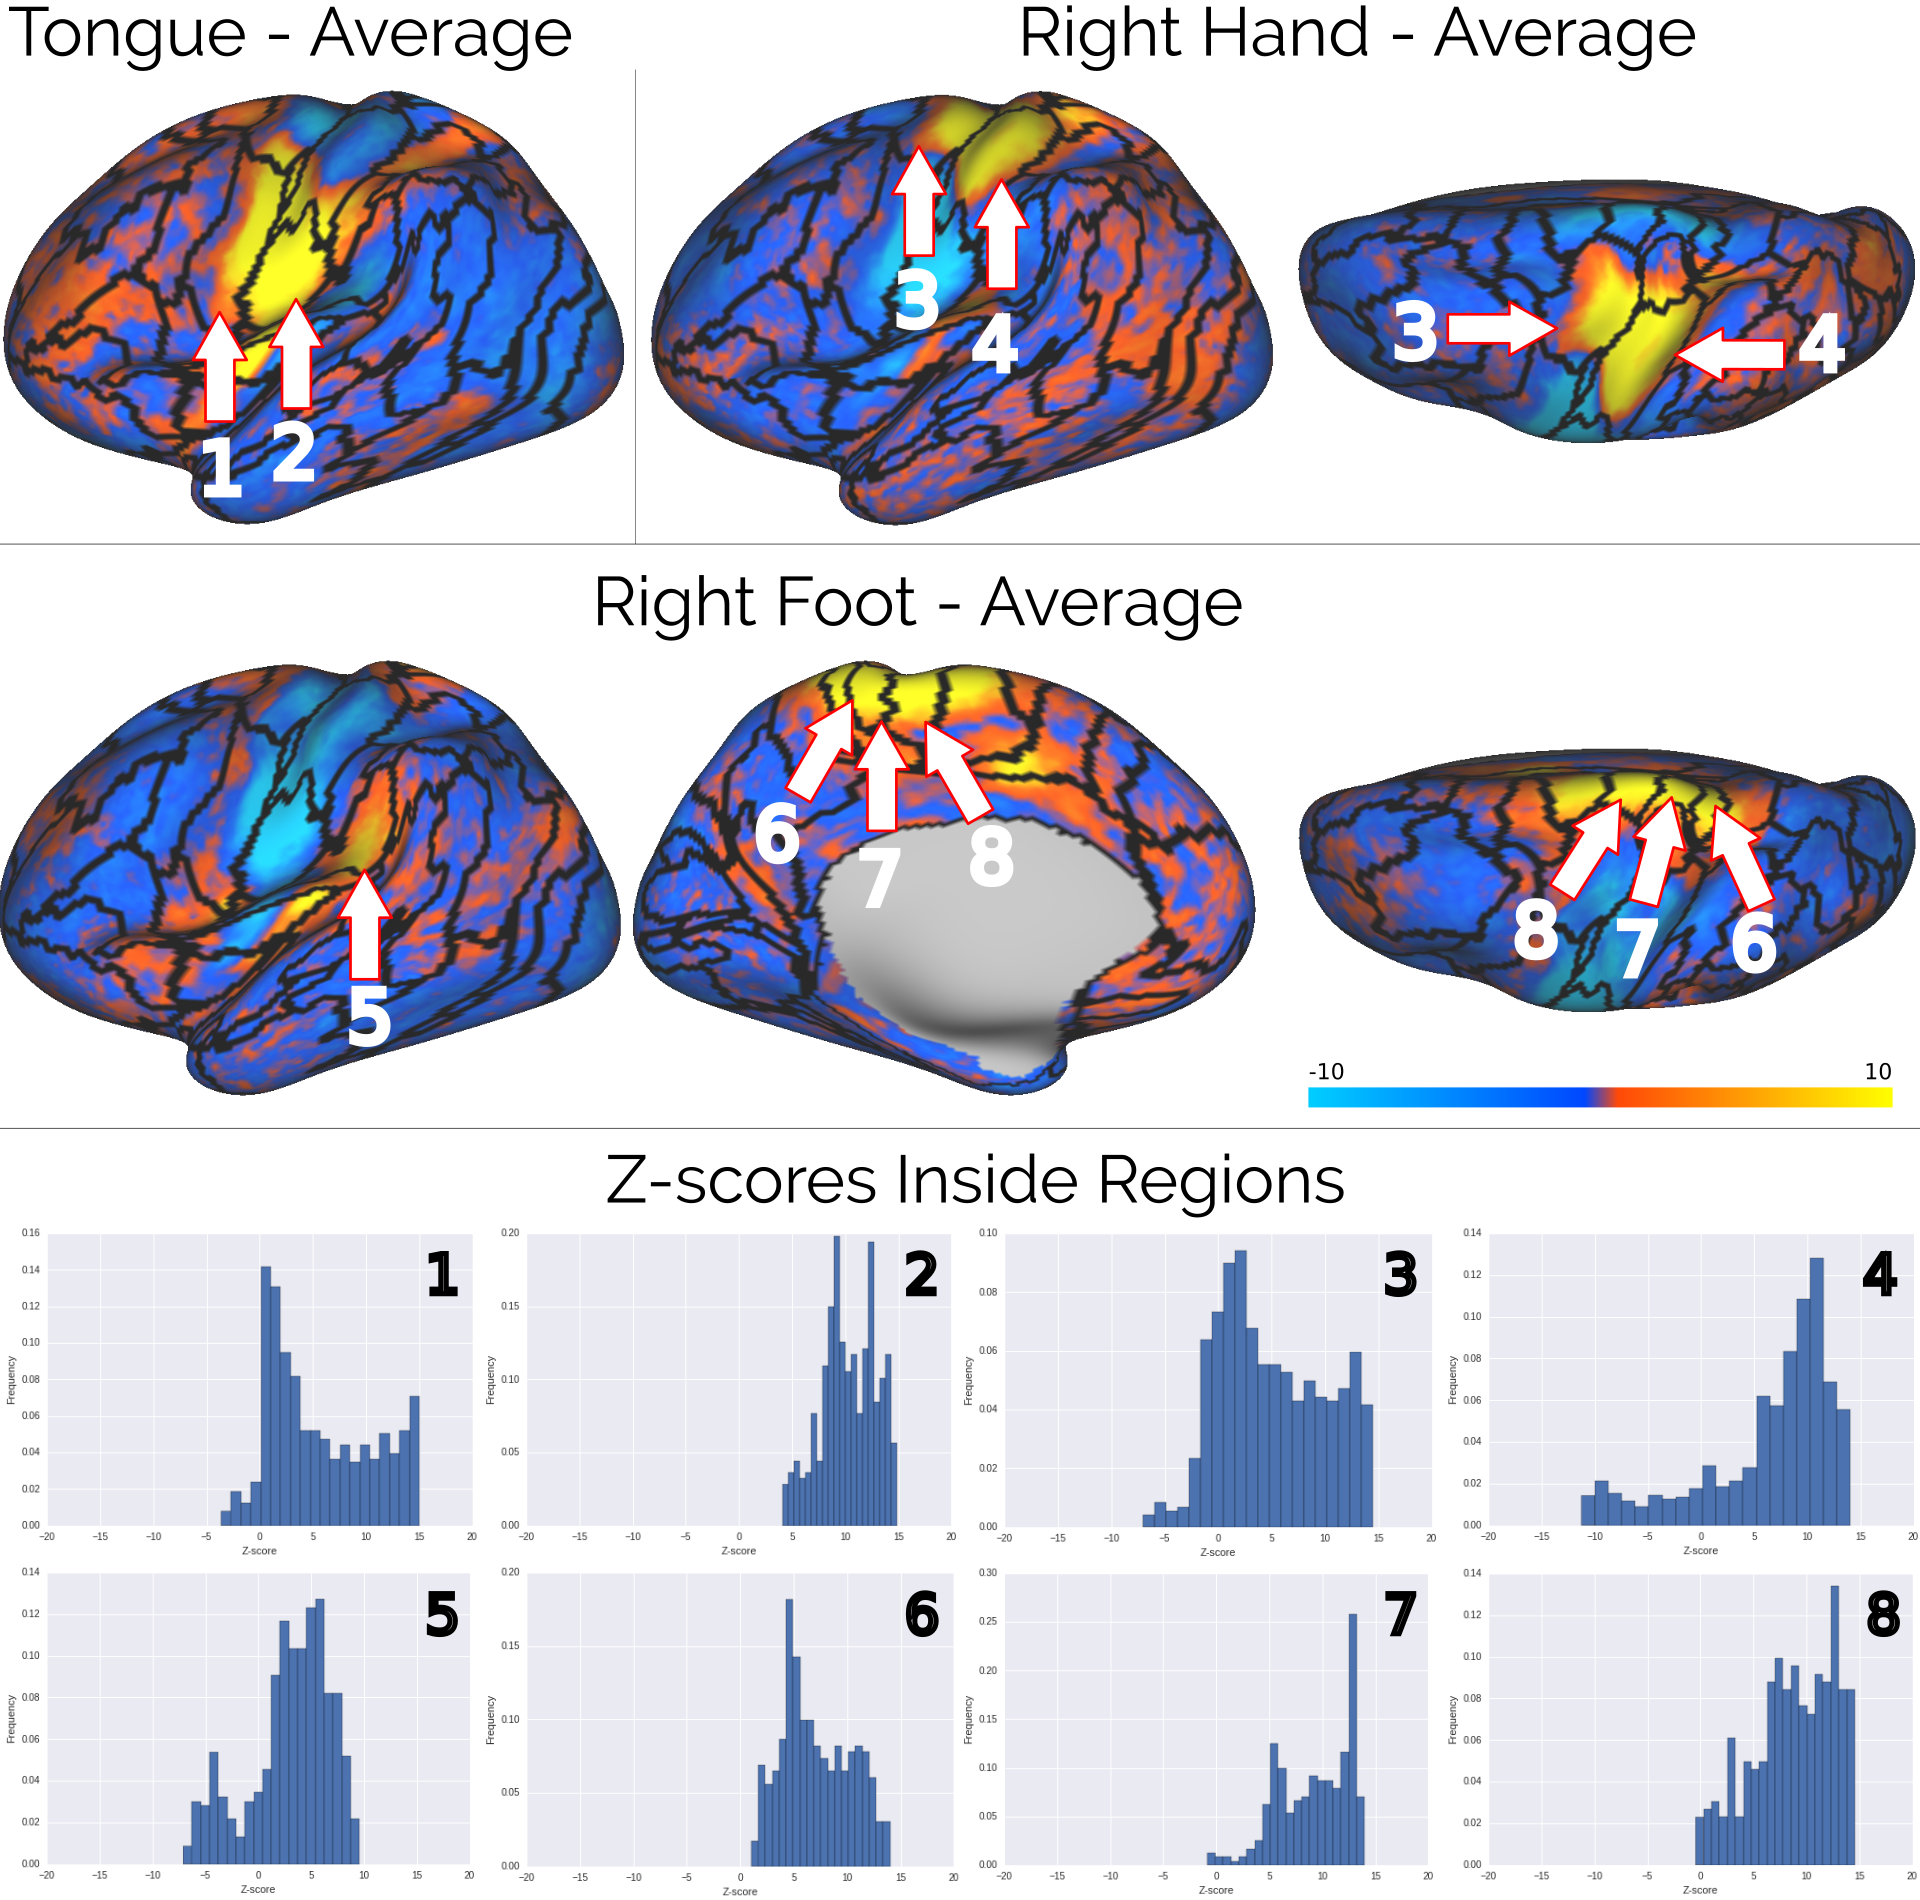
\includegraphics[width=\textwidth]{5.structural_clustering/img/function1.png}
    \caption{Our groupwise parcellation with 55 parcels projected over
             z-scores representing responses to motor tasks. Each histogram
             shows the distribution of z-score inside our parcels. The null or
             small fraction of negative values shows the functional specialization
             of our parcels}
    \label{fig:function_motor}
\end{figure*}

\begin{figure*}
    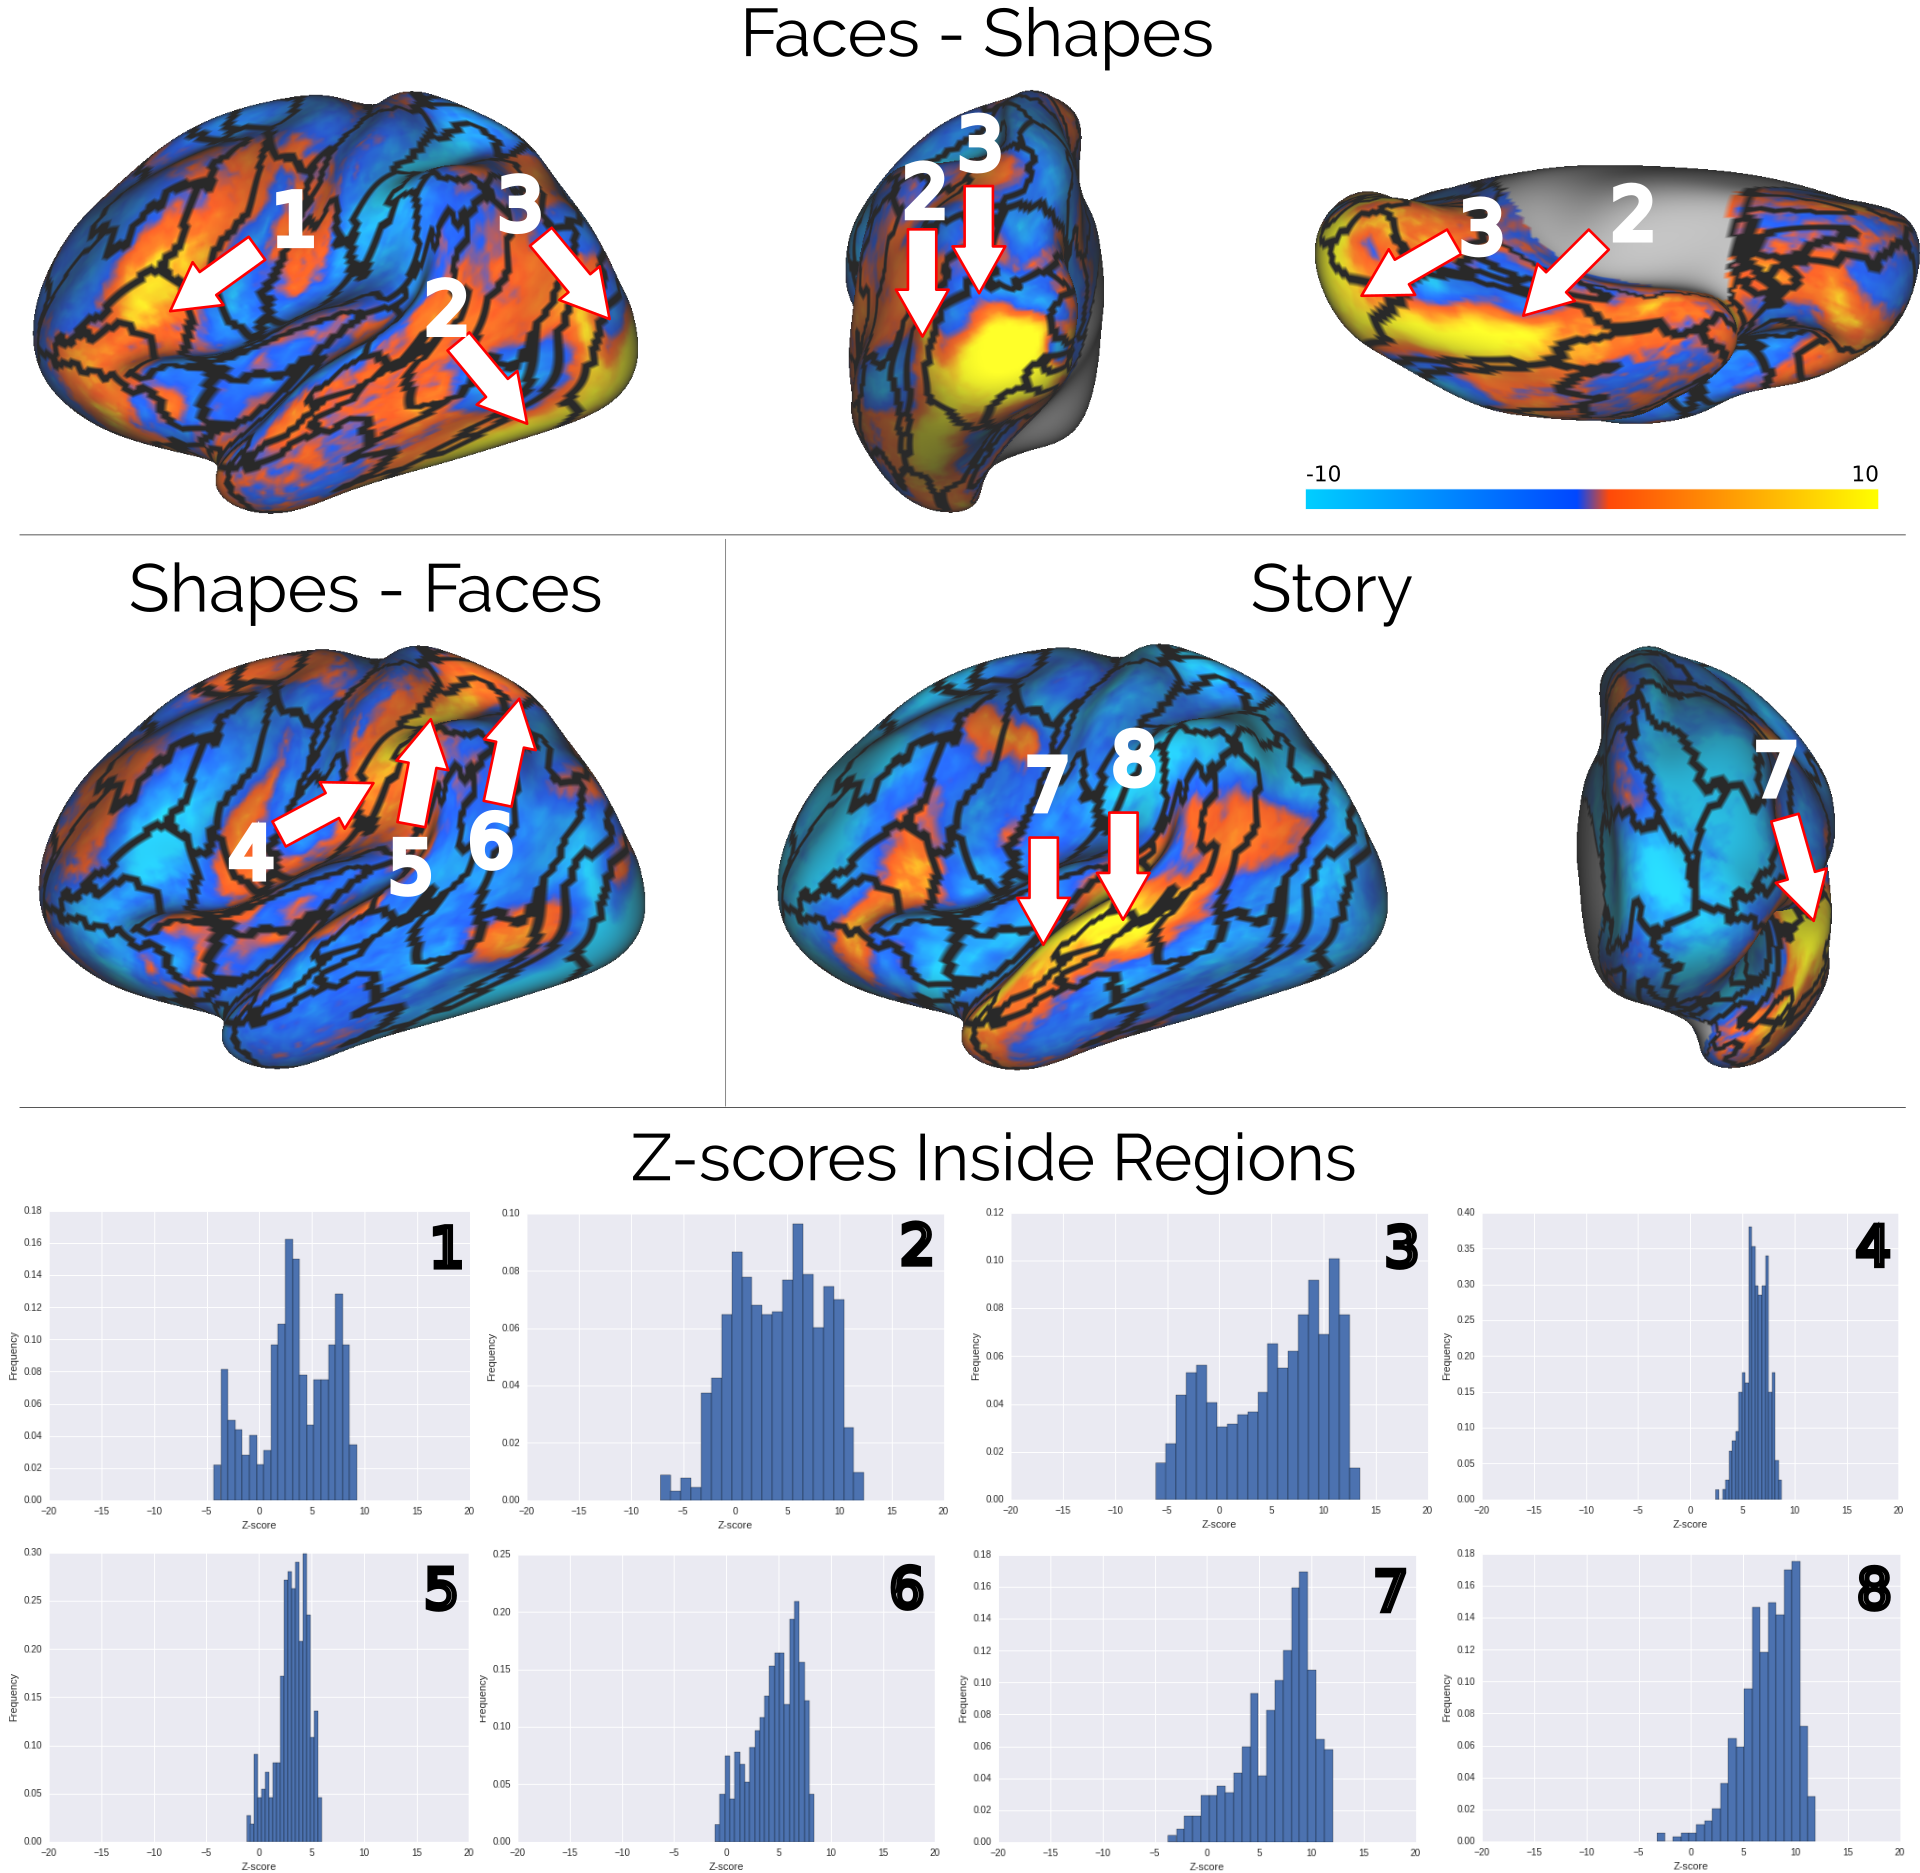
\includegraphics[width=\textwidth]{5.structural_clustering/img/function2.png}
    \caption{{Our groupwise parcellation with 55 parcels projected over
             z-scores representing responses to cognitive tasks. Each histogram
             shows the distribution of z-score inside our parcels. The null or
             small fraction of negative values shows the functional specialization
             of our parcels}
}
    \label{fig:function_cognition}
\end{figure*}

\begin{table*}[t]
\centering
\scalebox{0.9}{
  \begin{tabular}{@{}cccccc@{}}
      \multicolumn{6}{c}{\textbf{Table 2. Statistics on z-score distribution
                                 in parcels from figure
                                 \ref{fig:function_motor}}}  \\ \midrule
\textbf{Contrast} & \textbf{Parcel} & \textbf{Min.} & \textbf{Max.} & \textbf{Mean $\rpm$ Std. Dev.} & \textbf{Max. Score in Map}\\
T-Avg & \textbf{1} & -3.62  & 15.03 & $5.67 \rpm 4.91$ & 15.03 \\
T-Avg & \textbf{2} & 4.11 & 14.88 & 10.30 $\rpm$ 2.56 & 15.03 \\
RH-Avg & \textbf{3} & -7.02  & 14.50 & 5.05  $\rpm$ 4.95 & 14.50 \\
RH-Avg & \textbf{4} & -11.25  & 14.07  & 6.35 $\rpm$ 6.25 & 14.50\\
RF-Avg & \textbf{5} & -7.10 & 9.57& 2.99 $\rpm$ 3.84 & 14.56 \\
RF-Avg & \textbf{6} & 1.04& 14.01 & 7.13 $\rpm$ 3.20 & 14.56 \\
RF-Avg & \textbf{7} &-0.83 & 13.98& 9.23 $\rpm$ 3.32 & 14.56\\
RF-Avg & \textbf{8} &-0.46 & 14.56& 8.73 $\rpm$ 3.81 & 14.56 \\ \bottomrule
    \end{tabular}}
% 
\vspace{0.3cm}
\caption*{Table 2. Minimum; maximum and mean z-score contained by each of the
          parcels enumerated in figure \ref{fig:function_motor}. The highest 
          z-score of each map is reported to facilitate comparison. T-Avg: Tongue
          movement versus average; RH-Avg: Right Hand Movement versus average; RF-Avg: 
          Right Foot Movement versus average.}
\end{table*}

\begin{table*}[t]
\centering
\scalebox{0.9}{
  \begin{tabular}{@{}cccccc@{}}
      \multicolumn{6}{c}{\textbf{Table 3. Statistics on z-score distribution
      in parcels from figure \ref{fig:function_cognition}}} \\ \midrule
\textbf{Contrast} & \textbf{Parcel} & \textbf{Min.} & \textbf{Max.} & \textbf{Mean $\rpm$ Std. Dev.} & \textbf{Max. Score in map}\\
Faces-Shapes & \textbf{1} & -4.33 &  9.28 & 3.35 $\rpm$ 3.51 & 13.45 \\
Faces-Shapes & \textbf{2} & -7.16 & 12.36 & 4.01 $\rpm$ 4.09 & 13.45 \\
Faces-Shapes & \textbf{3} & -6.07 & 13.45 & 5.16 $\rpm$ 5.25 & 13.45 \\
Shapes-Faces & \textbf{4} & -5.73 &  5.37 & 0.93 $\rpm$ 1.78 &  8.79 \\
Shapes-Faces & \textbf{5} & -4.11 &  7.67 & 1.11 $\rpm$ 2.11 &  8.79\\
Shapes-Faces & \textbf{6} & -1.13 &  5.94 & 3.17 $\rpm$ 1.49 &  8.79 \\
Story & \textbf{7} & -3.72 & 12.02 & 6.72 $\rpm$ 3.35 & 12.02\\
Story & \textbf{8} & -3.24 & 11.92 & 7.41 $\rpm$ 2.50 & 12.02\\ \bottomrule
\end{tabular}}
% 
\vspace{0.3cm}
\caption*{Table 3. Minimum; maximum and mean z-score contained by each of the 
          parcels enumerated in figure \ref{fig:function_cognition}. The
          highest z-score of each map is reported to facilitate comparison. Faces-Shapes: 
          Face recognition versus shape recognition contrast; Shapes-Faces: Shape recognition
          versus face recognition; Story: Short story categorization.}
\end{table*}
%
\subsection{Relationship with a Multi-Modal Parcellation of the Cortex}
Finally, we study the (dis)similarities between our groupwise parcellation and that
of \citet{Glasser2016}. In their work, \citet{Glasser2016} compute a parcellation
of the whole cortex using information from different MRI modalities. In particular,
they use information from task functional MRI; resting state functional MRI;
myelin maps computed from T1 and T2 images and cortical thickness. It is important
to remark that dMRI data, in which our work is solely based, was not used to construct 
their parcellation.

\begin{figure*}
    \centering
    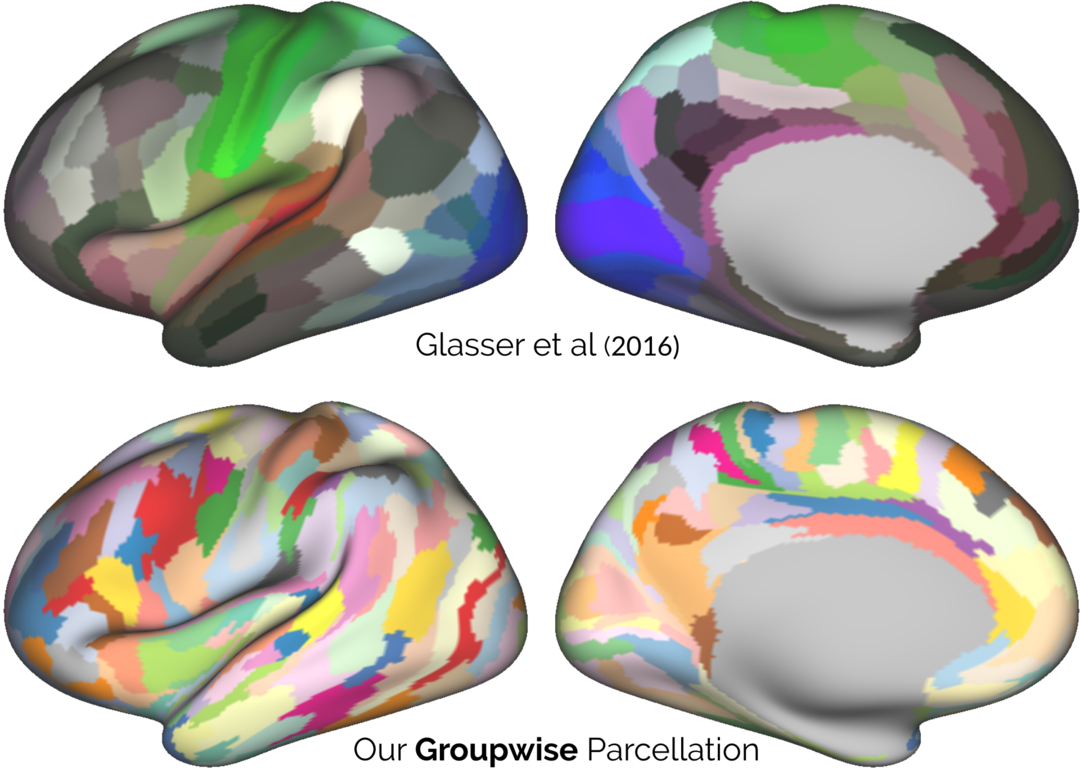
\includegraphics[width=\textwidth]{5.structural_clustering/img/glasser_and_me.png}
    \caption{\citet{Glasser2016} parcellation (upper) and our
    		 groupwise parcellations computed from 138 HCP subjects. Both 
             parcellations contain 180 parcels. There's almost no overlap according
             to the adjusted Rand index between them (0.28).}
    \label{fig:glasser_and_me}
\end{figure*}

To compare our results against Glasser's atlas, we first extracted a parcellation 
of 180 parcels from the groupwise dendrogram of our 138 HCP subjects. That is, we 
extracted a parcellation with the same number of parcels as Glasser's one. Figure
\ref{fig:glasser_and_me} show both parcellations side by side. 
We compared both parcellations using the adjusted Rand Index, obtaining a score
of 0.28. Such low score indicates that there's almost no similarity between our
result and that of \citet{Glasser2016}. Also, there's no relationship with
our groupwise parcellation with 55 parcels used in the previous section since
Glasser's parcels (finest) do not subdivide ours (coarsest).
Since Glasser's parcellation comes from functional information in the HCP, we
studied the functional specialization of its parcels in the same manner as 
previous section. Figure \ref{fig:glasser_functional} shows the histogram of
z-score contained for some parcels when using the same maps as in section
Functional Activations. It's important to remark that the z-score maps used
come from responses to functional stimuli of HCP subjects \citep{Glasser2013}.
In particular, histograms a; b and c in fig. \ref{fig:glasser_functional} show
that their subdivisions of the sensori-motor cortex contain a wide range of 
z-scores, centered in zero.

\begin{figure*}
    \centering
    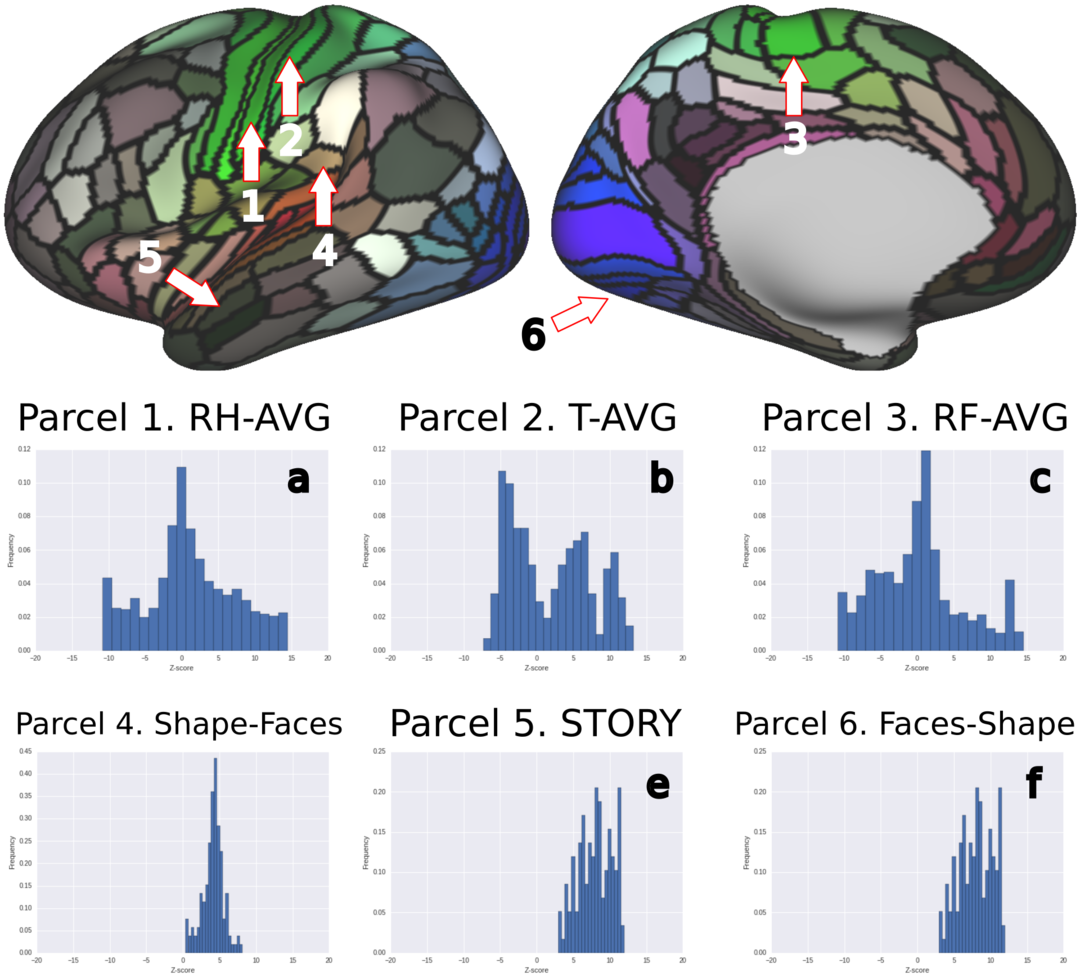
\includegraphics[width=\textwidth]{5.structural_clustering/img/glasser_functional.png}
    \caption{\citet{Glasser2016} parcellation (upper) and histograms of 
             z-score contained in different parcels for different functional
             task. (a) Histogram for parcel 1 for the contrast related to
             Tongue movement. (b) Histogram for parcel 2 for the contrast
             related to Tongue movement. (c) Histogram for parcel 3 for the
             contrast related to Right Foot movement. (d) Histogram for parcel
             4 for the contrast Shape recognition vs Face recognition. (e)
             Histogram for parcel 5 for the contrast related to Story
             Categorization.
             (f) Histogram for parcel 5 for the contrast Face recognition vs Shape
             recognition. The histograms (d); (e) and (f) correspond to the parcels
             with the greatest mean z-score of their respective tasks.}
    \label{fig:glasser_functional}
\end{figure*}
%
\section{Discussion}
%
In this work we presented a parsimonious statistical model for long-ranged
axonal connectivity. Our model (section \ref{sec:cortical_model}), assumes that
the cortex is divided in patches of homogeneous extrinsic connectivity, as histological
results showed in the macaque brain \citep{Schmahmann2006}. By borrowing ideas
from statistical clustered data models~\citep{Pendergast1996}, our model accounts
for the variability in the axonal connections of a patch's neurons and for 
variability in patch boundaries across subjects.

Taking advantage of our proposed model, in Section \ref{sec:parceling_methodologies}
we presented an efficient
technique to parcellate the cortex based on its extrinsic connectivity. Our
technique uses only dMRI information, without the need of relying on
initial parcellations~\citep{Clarkson2010}. Also, our technique allows 
parcellation of the whole cortex, overcoming the problem of working with only part
of it~\citep{Lefranc2016, Roca2009, ThiebautdeSchotten2014, ThiebautdeSchotten2016}.
Additionally, our technique allows creation of both single subject and
groupwise parcellations. Our groupwise parcellation technique relies on anatomical
seed-correspondence across subjects. In our experiments, this is achieved as
each HCP subject possess a coregistered dense mesh representing they cortical
surface \citep{Glasser2013}. Given the anatomical differences across-subjects,
this purely anatomical matching of seeds is probably sub-optimal. However, it
allows us to compute single and groupwise parcellations independently. By doing
this, we avoid the need to impose constraints between our single and group
parcellations~\citep{Clarkson2010, Roca2010, Paristot2015}.

Inspired by \citet{Moreno-Dominguez2014}, our technique uses Hierarchical
Clustering to comprise multiple granularities of the same parcellation in a
dendrogram. This allows us to overcome the need of other techniques~\citep{Paristot2015}
to specify an expected number of clusters. Hence, we don’t need to recompute the
whole pipeline each time a new parcellation is required. As in
\citet{Moreno-Dominguez2014}, we also create the dendrogram using only one
comprehensive parameter: the minimum size of each cluster. This
parameter imposes the local coherence criterion. Our fundamental difference
with Moreno-Dominguez' technique is how we compare and merge tractograms during
the clustering process. \citet{Moreno-Dominguez2014} use Centroid
Clustering~\citep{Murtagh1985} with the cosine distance. This can lead to an
erroneous parcellation since the centroid criterion doesn't minimize the cosine
distance between points. Also, their method creates dendrograms with inversions
\citep{Murtagh1985}, which are then removed heuristically. In our case, using a
Logistic Random Effect model (eq. \ref{eq:ran_eff_model}) allowed us to transform
the tractograms into a Euclidean space (sec. \ref{sec:parceling_methodologies})
and compare them using the Euclidean distance. In doing this, it is important to
remark that we are making a trade off. Since we are comparing high-dimensional
vectors with the Euclidean distance, we are probably affected by the dimensionality
curse \citep{Beyer1999}. However, working in an Euclidean space possess many
advantages. The first advantage is that we can compute clusters with minimum
intra-cluster variance by using Ward's Hierarchical method. We can use this algorithm
since its only hypothesis is that the features to cluster are in a Euclidean space.
Also, since we work with the Euclidean distance, we can apply the Lance and Williams
\citep{Lance} formula during clustering. This formula gives us the dissimilarity
between the new centroid created at each step and the rest of the existing
tractograms in constant time. As far as we know there's no Lance and Williams
formula when using the cosine distance with the centroid linkage. This allows
us to lower the time complexity of our algorithm with respect to Moreno-Dominguez.
Since we use Ward's clustering, our resulting dendrograms do not have
inversions, which means that we don't need to post-process them. Another
advantage is that we can retrieve a parcellation from the dendrogram using a
simple technique: horizontal cut~\citep{Murtagh2011}. While other methods to cut
the dendrogram exist~\citep{Murtagh2011}, horizontal cut is sufficient to solve
our Gaussian Mixture Model (eq. \ref{eq:ran_eff_model}) as shown in
\citet{Gallardo2017}. Finally, even if our algorithm is probably affected by
the dimensionality curse, our parcellations showed to be consistent
across-groups and in agreement with extant parcellations in the literature.
%
\subsection{Our Groupwise Parcellations are Consistent Across Similar Groups:}
%
We assessed the consistency of our groupwise parcellation by quantifying the
consistency across 3 disjoint groups of 46 subjects each. The consistency is
shown by the adjusted
Rand index in Fig.~\ref{fig:real_vs_fake}, which quantifies consistency across
parcellations~\citep{Hubert1985}. As seen in Fig.~\ref{fig:real_vs_fake} whole-cortex
parcellations obtained with our method are consistent across groups, and the
Adjusted Rand Index is significantly higher, i.e.\ more than 3 standard
deviations, for all granularities when compared with the null case of
randomly-generated parcellations. 

Our whole-cortex groupwise parcellation reaches a maximum consistency score when
the cortex is divided in 6 regions, see Fig.~\ref{fig:real_vs_fake}.  As seen in
Fig. \ref{fig:groups}, these parcellations are consistent with specific
anatomo/functional networks: the frontal lobe section anterior to the prefrontal
cortex is shown in yellow; the sensorimotor area is shown in cyan, the cingulate
area is shown in beige; the fronto-occipital connection in orange, and the
temporo-parietal system in pink. 

\subsection{Our Method Creates Parcels in Agreement With a Single-Lobe Parceling
            Technique Extant in the Literature.}
%
We showed that our technique obtains results similar to another method extant
in the literature. We did so by parceling only the frontal and showing the visual
similarity between our resulting parcels and those obtained by
\citet{ThiebautdeSchotten2016}. Moreover, the blue, pink and green parcels
in fig. \ref{fig:frontal} share not only similar boundaries and location, but
also functional specialization (Table 1). In some cases our parcels possess even higher
spatial-correlation with functional task according to
Neurosynth's \citep{Yarkoni2011} Decode tool\footnote{http://neurosynth.org/decode/}. We assessed the 
consistency of our obtained groupwise parcellation by computing the groupwise 
frontal lobe parcellation of three disjoints groups of 46 subjects and comparing
them using the adjusted Rand index. The obtained value of $0.61$ shows that our
parcellation of the frontal lobe is consistent across groups.
%
\subsection{Our Method Creates Several Parcels in Agreement with Brain Anatomy.}
%
We showed that many of our parcels are in agreement with brain anatomy. 
In particular, we showed that in our groupwise parcellation, with 55 parcels,
the following anatomical structures appeared to be found: Cingulate; Insula;
Lateral-Occipital; Fusiform; Superior Frontal; Lingual; Motor and Sensory cortex.
Here we discuss why some of these parcels were found and how are their 
conectivity fingerprints.
In the case of the Cingulate, its fingerprint, shown in fig. \ref{fig:conn_fing}, is
strongly related with the Cingulate Fascicle (CF) pathway. This
is consistent with the 
fact that the seeds located in the Cingulate will end up into the CF after being 
pushed in the white-matter. In the case of the Insula, each subdivision
showed a specific pattern of connectivity as shown in fig. \ref{fig:conn_fing}. 
These parcels show a gradient of connections from the occipital lobe to the frontal
lobe consistent with that of \citet{Ghaziri2015}. In the
Lateral-Occipital region, we see a specific pattern of local connectivity which
cannot be attributed to gyral bias since the Lateral-Occipital covers many sulci
and gyrus. In the case of the fusiform, it is almost completely contained in one
of our parcellations, which goes from the Fusiform up to the Lateral-Occipital
(fig. \ref{fig:anatomical_zoom}). 
This could add evidence to the hypothesis that the Fusiform plays a role in visual
tasks \citep{Kanwisher2006, Yeatman2014}. Finally, the Motor and Sensory cortex appear to be
found. While the
appearance of each gyri is most probably because of gyral bias \citep{VanEssen2014},
the parcels inside them show specific patterns of structural connectivity (fig.
\ref{fig:conn_fing}), and, as seen in section 3.5.2, functional specialization.

\begin{figure*}
    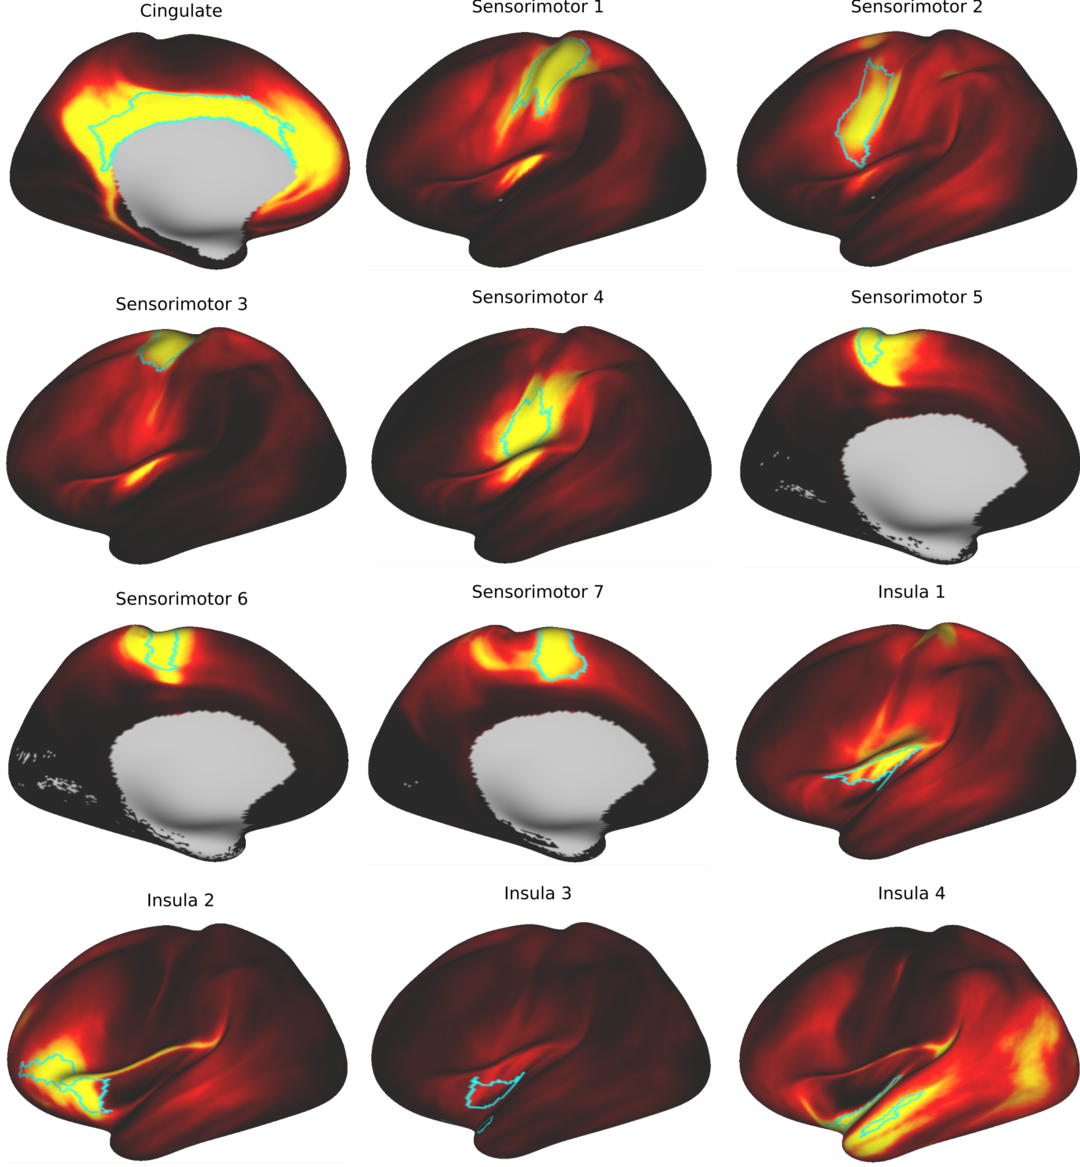
\includegraphics[width=\textwidth]{5.structural_clustering/img/conn_fing.png}
    \caption{Connectivity fingerprint for different parcels in our groupwise
             parcellation. The names in the titles are given after the anatomical
             structure that they subdivide (or contain, as with the Fusiform). }
    \label{fig:conn_fing}
\end{figure*}


\subsection{Our Results Show a Close Relationship Between Structural Connectivity
and Brain Function.}
%
We assessed the functional specialization of some of our parcels by showing
how they overlap with responses to functional and cognitive tasks measured
with fMRI. In particular, for all the studied tasks, the parcels contained
a higher proportion of positive values than negative ones as expressed by the
positive mean values reported in tables 2 and 3. For some parcels there
were not even negative values. Moreover, several of the histograms on figures
\ref{fig:function_motor} and \ref{fig:function_cognition} show a high frequency
of z-score values greater than 5, which indicate a significant correlation with
functional activation. Therefore, our results show, for some tasks, the
strong relationship between extrinsic connectivity and functional
specialization in the human brain cortex. 
%
\subsection{Our Parcels Are Not Similar to Those Obtained by Glasser et al. (2016) But 
			Possess Better Functional Specialization for Motor Tasks.}
Our parcels were not related to those of \citet{Glasser2016}. This is shown by the
obtained adjusted Rand index score between them (0.28). It's important to remark that
our parcels are purely based on extrinsic connectivity, meanwhile those of \citet{Glasser2016}
do not use dMRI information. Glasser's parcels are mostly based on myelin and functional information.
In particular, their subdivision of the sensori-motor cortex (green parcels in fig.
\ref{fig:glasser_and_me}) is mostly based in Myelin maps as shown in Figure 4.a of 
\citet{Glasser2016}. Because of this, their parcels in the sensori-motor cortex contain 
a wide range of z-scores when compared with responses to functional stimuli as shown by
histograms a; b and c in fig.
\ref{fig:glasser_functional}. In contrast, our parcels in the sensori-motor cortex,
for a coarser parcellation, show a good overlap with function and are in agreement with
the motor strip mapping as discussed in the previous section. Also, for the case of story
categorization; shape recognition and face recognition, our parcels show a similar
distribution of z-scores (fig. \ref{fig:function_motor}) than those with the highest 
mean z-scores of \citet{Glasser2016} (parcels d; e and f of  fig. \ref{fig:glasser_functional}).
%
\section{Conclusion}
%
Understanding how the brain is structurally organized and how it constraints
functionality is an open question in neuroscience. Recent advances in
acquisition and modeling techniques on dMRI have facilitated to study 
axonal connectivity in the brain. However, parceling the whole cortex based
on a structural criterion remained challenging. In this chapter we presented a 
connectivity model; framed tractography within our model and 
presented a parceling technique that allows parcellation
of the whole brain in both single subject and groupwise cases.

However, a new question rises, given two single subject parcellations, how to
match the parcels across them?. Even when our results show that our technique is stable
across groups of subjects, some variability still exists, and finding a
correspondence between two parcellations is not a trivial task. The 
following chapter of this thesis will work on this problem.

%\section{References}
%\bibliographystyle{elsarticle-harv}
\chapterbib


%%%% BIBLIOGRAFIA
%\bibliography{bibliography}

\end{document}
